%\UseRawInputEncoding

\documentclass[11pt,twoside,singlespace]{report}

\setlength{\topmargin}{0pt}
\setlength{\textheight}{619pt}				
\setlength{\oddsidemargin}{18pt}	
\setlength{\evensidemargin}{18pt}	
\setlength{\textwidth}{432pt}	
\usepackage[T1]{fontenc}
\usepackage{amssymb,amsmath} 
\usepackage{graphicx}
\usepackage{tabularx}  
\usepackage{longtable}
\usepackage{verbatim}  
\usepackage[usenames]{color}
\usepackage[square]{natbib}
\usepackage{fancyhdr}
\usepackage{url}
\usepackage[colorlinks=true,allcolors=blue,linkcolor=blue]{hyperref}
\usepackage{bm}
\usepackage{float}
\usepackage{tcolorbox}
\usepackage{hhtensor}
\usepackage{xstring}

\graphicspath{{figures/}}

\DeclareRobustCommand*\matr[1]{\ushortd{#1}}
\DeclareRobustCommand*\vec[1]{\ushort{#1}}

\newcommand{\notf}{{\ttfamily .NOT.}}
\newcommand{\true}{{\ttfamily .TRUE.}}
\newcommand{\false}{{\ttfamily .FALSE.}}
\newcommand{\KNOSOS}{{\ttfamily KNOSOS}}
\newcommand{\TASKTD}{{\ttfamily TASK3D}}
\newcommand{\NEOTWO}{{\ttfamily NEO2}}
\newcommand{\PENTA}{{\ttfamily PENTA}}
\newcommand{\DKES}{{\ttfamily DKES}}
\newcommand{\COTRANS}{{\ttfamily COTRANS}}
\newcommand{\VMEC}{{\ttfamily VMEC}}
\newcommand{\NEOTRANSP}{{\ttfamily neotransp}}
\newcommand{\SFINCS}{{\ttfamily SFINCS}}
\newcommand{\EUTERPE}{{\ttfamily EUTERPE}}
\newcommand{\FORTEC}{{\ttfamily FORTEC-3D}}
\newcommand{\BOOZERXFORM}{{\ttfamily BOOZER\_XFORM}}
\newcommand{\NEO}{{\ttfamily NEO}}
\newcommand{\MPI}{{\ttfamily MPI}}
\newcommand{\FFTW}{{\ttfamily FFTW}}
\newcommand{\PETSC}{{\ttfamily PETSc}}

\newcommand{\todo}[1]{\textcolor{red}{#1}}
\newcommand{\tocheck}[1]{\textcolor{blue}{#1}}

\newcommand{\epsi}{\mathbf{e}_\psi}
\newcommand{\epol}{\mathbf{e}_\theta}
\newcommand{\epolt}{\mathbf{e}_{\tilde{\theta}}}
\newcommand{\etor}{\mathbf{e}_\zeta}
\newcommand{\bb}{\mathbf{b}}
\newcommand{\bB}{\mathbf{B}}
\newcommand{\bE}{\mathbf{E}}
\newcommand{\fsa}[1]{\left\langle{#1}\right\rangle}
\newcommand{\bv}{{\mathbf{v}}}
\newcommand{\bnabla}{\mathbf{\nabla}}
\newcommand{\tbl}{\textbackslash}

\newcommand{\makesub}[1]{%
  \saveexpandmode\noexpandarg
  \StrSubstitute{#1}{\_}{_}[\temp]%
  \restoreexpandmode
}
\newcommand{\mytarget}[1]{%
  \makesub{#1}%
  \hypertarget{\temp}{#1}%
}
\newcommand{\mylink}[1]{%
  \makesub{#1}%
  \hyperlink{\temp}{#1}%
}

\newcommand{\vlink}[1]{{\ttfamily \mylink{#1}}}

\newcommand{\ivarl}[7]{\horiz\begin{table}[H]\begin{tabularx}{\textwidth}{lX}
{\ttfamily \bfseries \mytarget{#1}} &  \\ [0cm]
{\it Purpose:} & #2  \\ [-0.2cm]
{\it Type:} & #3  \\ [-0.1cm]
{\it Effect if \true:} & #4  \\ [-0.2cm]
{\it Default value:} & #5  \\ [-0.2cm]
{\it Misc.:} & #6 \\ [-0.2cm]
{\it Ref.:} & #7
\end{tabularx}\end{table}}

\newcommand{\ivar}[7]{\horiz\begin{table}[H]\begin{tabularx}{\textwidth}{lX}
{\ttfamily \bfseries \mytarget{#1}} &  \\ [0cm]
{\it Purpose:} & #2  \\ [-0.2cm]
{\it Type:} & #3  \\ [-0.2cm]
{\it Effect:} & #4  \\ [-0.2cm]
{\it Default value:} & #5  \\ [-0.2cm]
{\it Misc.:} & #6 \\ [-0.2cm]
{\it Ref.:} & #7
\end{tabularx}\end{table}}

\newcommand{\horiz}{{\vskip-0.1cm\setlength{\parindent}{0cm} \hrulefill }\vskip-0.1cm}

\begin{document} 

%Cover page and table of contents
\begin{center}

{\Huge \textbf{KNOSOS}:} \\
\vskip0.5cm
{\LARGE \textbf{K}i\textbf{N}etic \textbf{O}rbit-averaging \textbf{SO}lver for \textbf{S}tellarators}

\vskip0.5cm

\begin{figure}[h]
\begin{center}
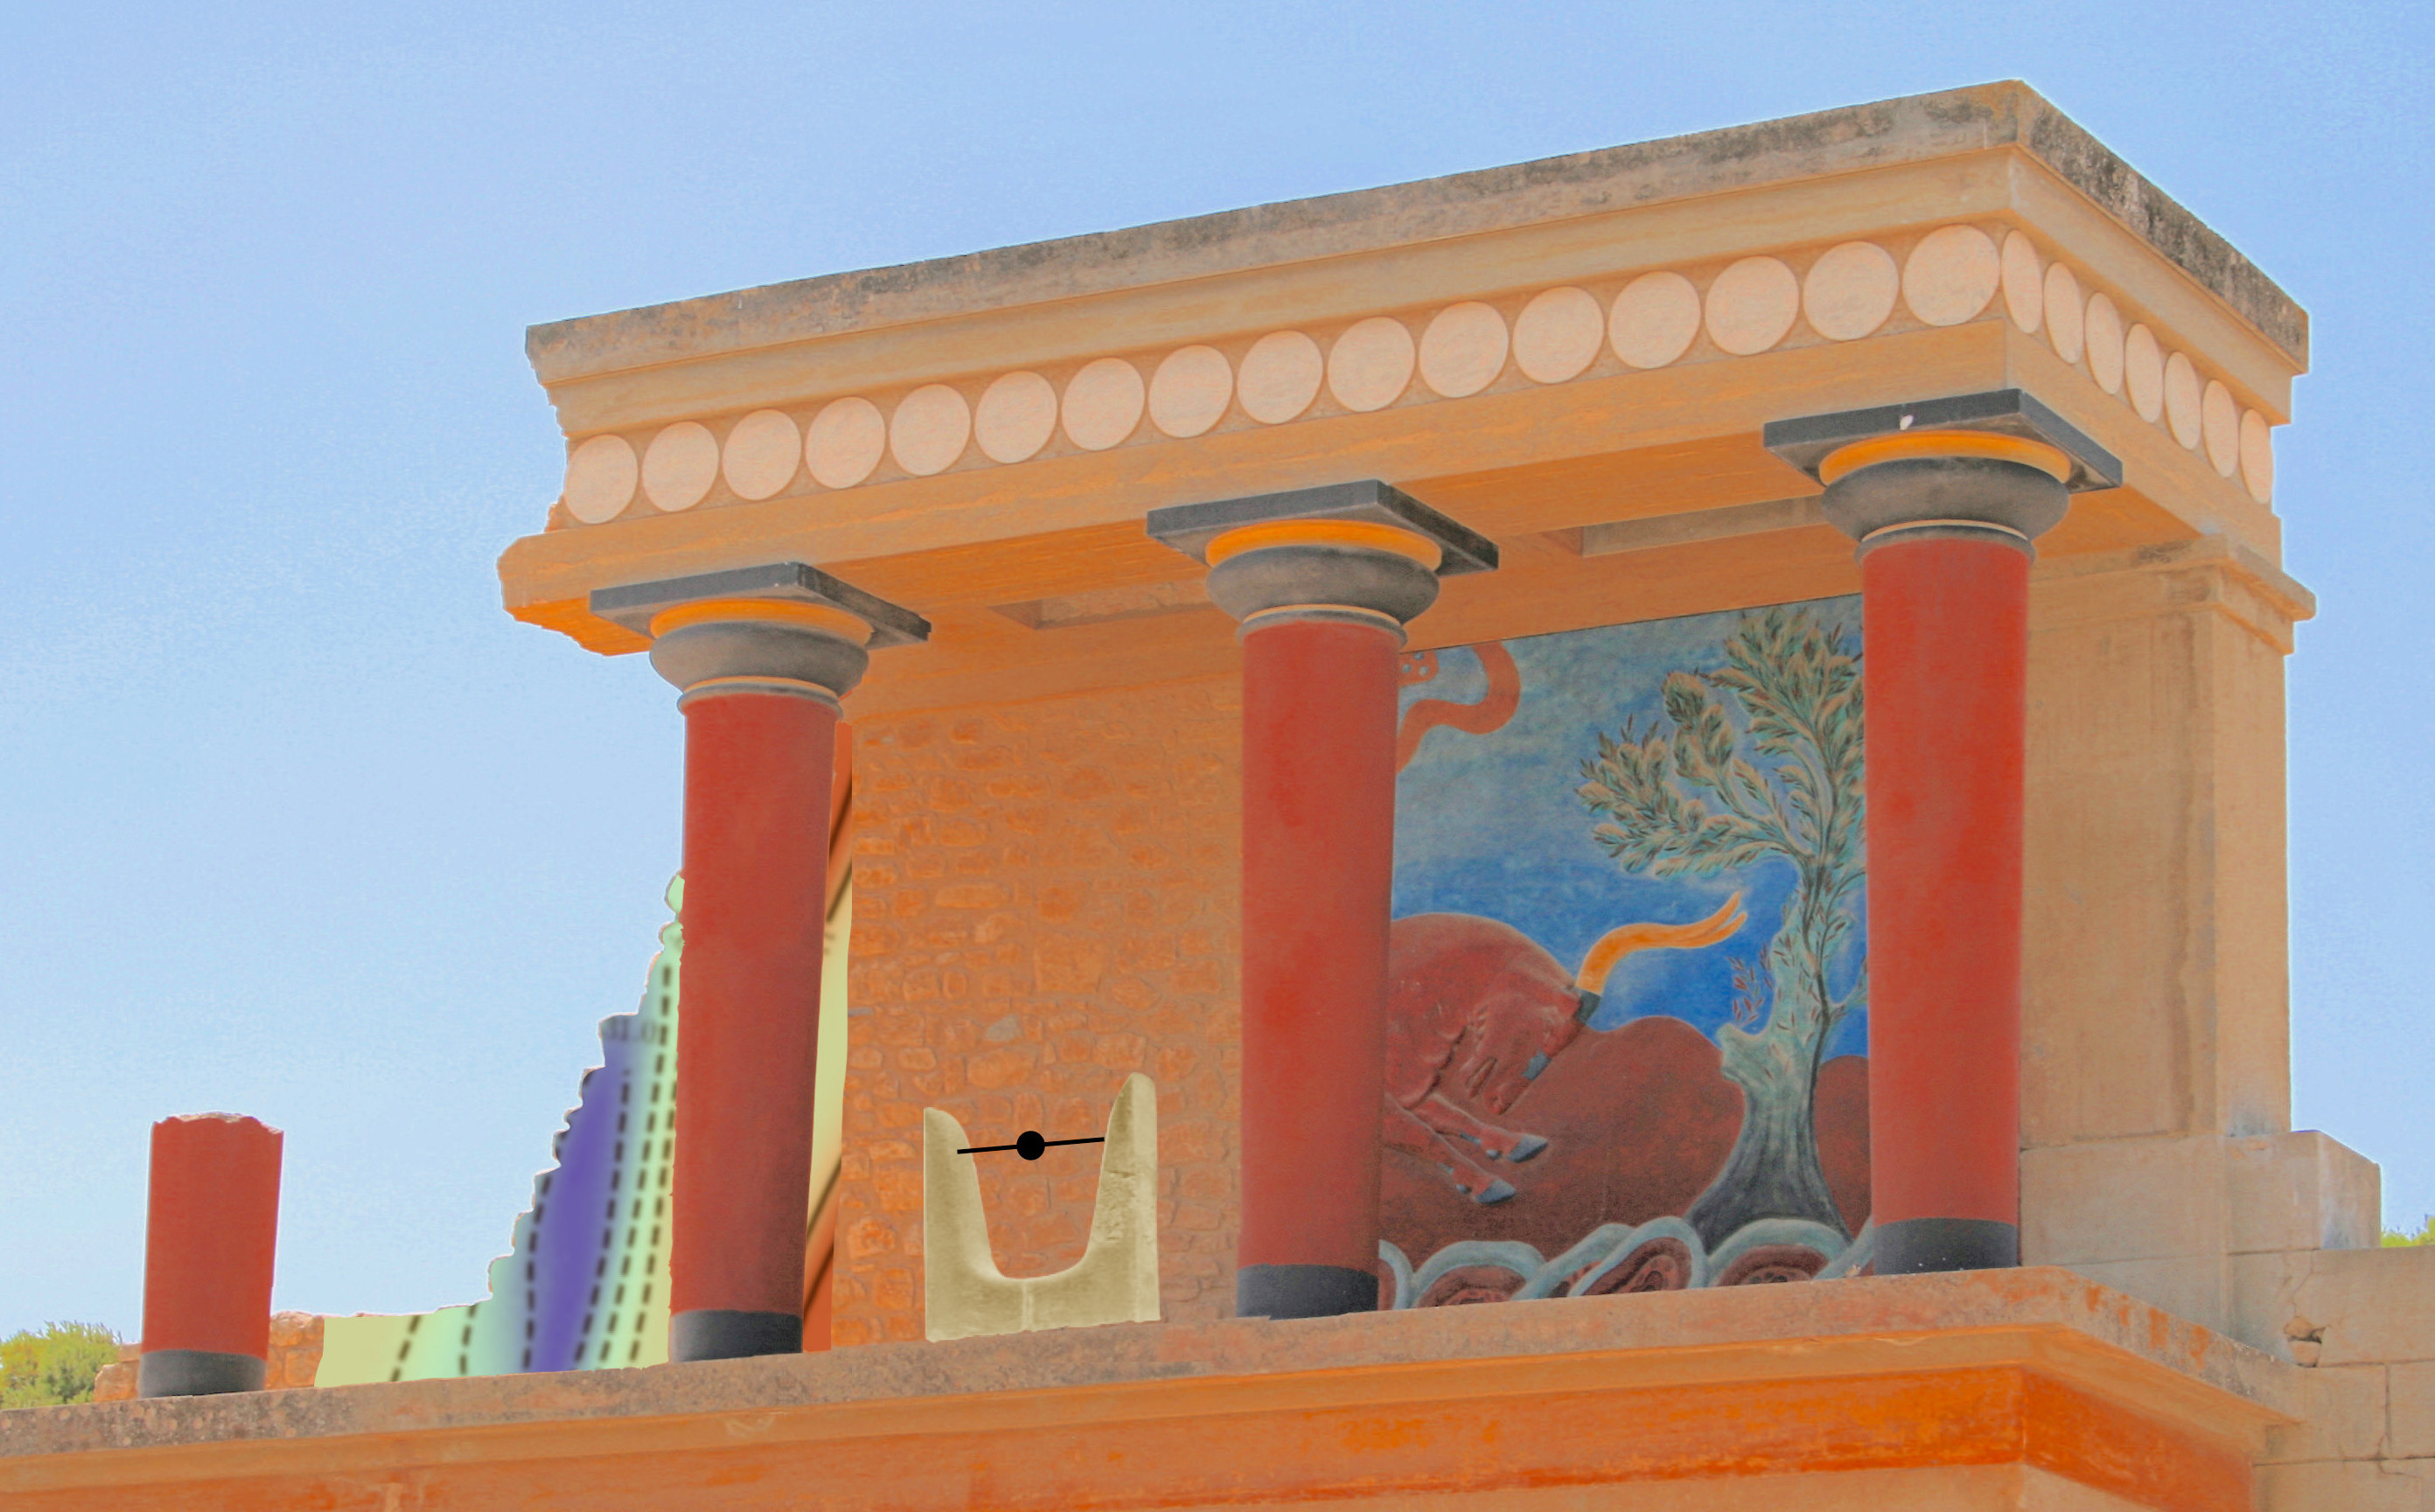
\includegraphics[width=1.0\textwidth]{knosos_logo_new}
\end{center}
\end{figure}


{\Large Technical Documentation and User Manual}

\vspace{0.5in}


Version 1 (last revised, \today)

\end{center}



\fancyhf{}
\cfoot{\thepage}


\

\

\

\

\

\

\


\normalsize
\begin{tcolorbox}[colback=gray!5,colframe=gray!40!black]

\

%\KNOSOS~is an open-source code freely available at 
%
%\
%
% \url{https://github.com/joseluisvelasco/KNOSOS}
%
%\
%
%You are very welcome to use it and/or to contribute to its development. It is also under continuous development, which means that,  although it has benchmarked, it might contain minor bugs and that its documentation may be incomplete. We are very happy to receive any feedback, which you can send us to 


\KNOSOS~is a freely available open-source code. You are very welcome to use it and/or to contribute to its development. It is also under continuous development, which means that, although it has been benchmarked, it might contain minor bugs and that its documentation may be incomplete. We are very happy to receive any feedback, which you can send us to 

\

\href{mailto:joseluis.velasco@ciemat.es}{\nolinkurl{joseluis.velasco@ciemat.es}}.

\

\

\KNOSOS~is part of a long-term project$^*$ aimed at the study of kinetic transport of multispecies plasmas of stellarators, in collaboration with researchers from the National Fusion Laboratory at CIEMAT (Spain), the University of Oxford (United Kingdom), the Max-Planck Institute for Plasma Physics, Greifswald (Germany) and the National Institute for Fusion Science (Japan). You can learn about our work and interests, which cover topics from the theory of energy transport in optimized stellarators to the experimental validation of impurity transport modelling in real stellarators, on our website

\

\href{http://fusionsites.ciemat.es/multitranstell//}{\nolinkurl{http://fusionsites.ciemat.es/multitranstell/}}, 

\

on the websites of our previous projects

\

\href{http://fusionsites.ciemat.es/stellaratortransport/}{\nolinkurl{http://fusionsites.ciemat.es/stellaratortransport/}}, 

\href{http://fusionsites.ciemat.es/kinetictransport/}{\nolinkurl{http://fusionsites.ciemat.es/kinetictransport/}},

\

and  on the personal website

\

\href{http://fusionsites.ciemat.es/jlvelasco/}{\nolinkurl{http://fusionsites.ciemat.es/jlvelasco/}}.

\

\

\footnotesize{$^*$ The work is carried out within the framework of the EUROfusion Consortium and has received funding from the Euratom research and training programme 2014-2018 under grant agreement No 633053. The views and opinions expressed herein do not necessarily reflect those of the European Commission. It has also been supported in part by grant ENE2015-70142-P of the Ministerio de Econom\'ia y Competitividad, Spain, and by grant PGC2018-095307-B-I00, Ministerio de Ciencia, Innovaci\'on y Universidades, Spain.}

\


\end{tcolorbox}







\tableofcontents 
\clearpage  
\pagestyle{fancy}
\fancyhf{}
\lhead[\thepage]{\leftmark}
\rhead[\leftmark]{\thepage}
\renewcommand{\chaptermark}[1]{\markboth{\sc{\chaptername\ \thechapter.\ #1}}{}}
\setlength{\headsep}{6pt}
\setlength{\parskip}{0pt plus 0pt minus 0pt}
\renewcommand*{\thefootnote}{\fnsymbol{footnote}}
%\UseRawInputEncoding

%Contents
\chapter{Introduction}

\KNOSOS~~(KiNetic Orbit-averaging SOlver for Stellarators) is a freely available, open-source code that calculates local neoclassical transport (i.e. transport caused by inhomogeneties of the magnetic field and collisions) in low-collisionality plasmas of three-dimensional magnetic confinement devices. This includes stellarators (helias, heliotrons, quasisymmetric devices, heliacs...) and perturbed tokamaks.

The main difference with respect to other local neoclassical codes is that \KNOSOS~relies on the orbit-averaging technique, which makes it very fast, since it allows to remove one of the coordinates of the problem. The code solves a drift-kinetic equation for each species with two independent variables: the angle $\alpha$ that labels magnetic field lines on a flux-surface and the pitch angle $\lambda$; the radial coordinate $\psi$ and the particle speed $v$ are parameters, and the gyro-angle and the spatial coordinate along the magnetic field line $l$ have been removed by gyro-averaging and orbit-averaging of the equations, respectively. It should be emphasized that, as we will discuss in forthcoming chapters, orbit-averaging does not imply a simplification on the treatment of the magnetic geometry of the stellarator: it can be done rigorously, and the code recovers, for real stellarators and at low collisionalities, the results (radial fluxes, variation of the electrostatic potential along the flux-surface, etc) of local neoclassical codes that do not perform orbit-averaging.

After this short overview, the rest of the manual is organized as follows: chapter~\ref{CHAP_MOT} explains the motivation and scope of this project. Chapter~\ref{CHAP_EQ} presents the equations solved by the current version of \KNOSOS, using methods described in chapter~\ref{CHAP_SOL}. Chapter~\ref{CHAP_INST} contains the instructions to set up the code, and chapter~\ref{CHAP_RUN} shows how to run it. The details are given in the rest of the manual: chapter~\ref{CHAP_INPUT} lists the input files and their variables, chapter~\ref{CHAP_PROF} describes how the plasma profiles are read and processed, and chapter~\ref{CHAP_CONF} does the same thing with the magnetic configuration; chapter~\ref{CHAP_OUTPUT} lists the output files and describes their content. Finally, chapter~\ref{CHAP_EX} shows some examples of simulations that can be reproduced by the user. Chapter~\ref{CHAP_CONC} provides some concluding remarks, and there are two appendices: appendix~\ref{CHAP_HIGHCOL} derives the additional equations that are solved for high-collisionality regimes; appendix~\ref{CHAP_DKES} shows how to use~\DKES~results as input for~\KNOSOS, or how to compare monoenergetic simulations of the two codes.

\

This manual describes ``version 1'' of \KNOSOS~, the one used in~\citep{velasco2019knosos}\footnote{The source code itself has also comments, but they often look like~\href{https://twitter.com/bercut2000/status/1009709520220803072?s=19}{this}.}. We note that the code is still under development.
\section{Main features}

Below we list the main features of the code, which will be explained in detail in later chapters:

\begin{itemize}

\item \KNOSOS~can read realistic magnetic equilibria in Boozer coordinates, generated e.g. with \VMEC~plus \BOOZERXFORM~or \COTRANS, as well as model magnetic fields.

\item Bounce-averaging, combined with the monoenergetic approximation, reduces the number of variables to 2 (to be compared to 3 in the case of \DKES, 4 in radially local codes such as \EUTERPE~and \SFINCS, and 5 in radially global codes such as~\FORTEC). This makes the code very fast, while retaining the physics necessary to describe important features of neoclassical transport at low collisionalities. 

\item In particular, the magnetic drift tangential to the flux-surface, which gives rise to the superbanana-plateau regime, can be retained, including the effect of the magnetic shear.
\begin{itemize}
\item These calculations have been benchmarked against~\todo{\FORTEC}\footnote{\todo{Red color means "to do" or "in progress".}} and analytical expressions.
\end{itemize}

\item The variation of the electrostatic potential on the flux-surface $\varphi_1$ can be calculated by solving consistently the drift-kinetic and the quasineutrality equations. The computing time is $\sim$1 minute in a single computer.
\begin{itemize}
\item These calculations have been benchmarked against~\EUTERPE.
\end{itemize}

\item The code typically calculates the radial fluxes for given input density and temperature profiles, but it can also provide a set of \textit{monoenergetic} transport coefficients for later use by transport solvers. The computing time is $\sim$seconds in a single computer.
\begin{itemize}
\item These calculations have been benchmarked against~\DKES.
\end{itemize}

\item \KNOSOS~can calculate the effective ripple in the same manner as \NEO~does, but it can also provide figures of merit of neoclassical transport for low-collisionality regimes different than the 1/$\nu$ (namely, the $\sqrt{\nu}$ and \todo{superbanana-plateau} regimes).

\item The calculated fluxes are moments the distribution function, which is explicitly computed and \todo{can be provided} in the output, for its use by e.g. gyrokinetic codes.

\item KNOSOS~has been combined with analytical formulas to provide fast computations of impurity transport in several neoclassical regimes.

\item  {\todo{\KNOSOS~can be used from the~\NEOTRANSP~suite developed at IPP and from from the~\TASKTD~suite developed at NIFS.}}

\end{itemize}


\section{Limitations}

\begin{itemize}

\item \KNOSOS~assumes that closed magnetic surfaces exist; magnetic islands and regions of stochastic fields or open field lines cannot be described.
\begin{itemize}
\item Regions in which the rotational transform is close to being a (low-order) rational number \todo{may be} numerically hard to converge.
\end{itemize}

\item The bounce-averaged technique is limited to low collisionalities: if the contribution from the plateau or Pfirsch-Schl\"uter regimes is not negligible, the calculation with~\KNOSOS~will not be accurate. 

\begin{itemize}
\item The appendices describe semianalytical methods to cover these regimes. 
\item \KNOSOS~can be used in combination with~\DKES~and then employed to calculate the radial fluxes for arbitrary collisionality correctly including the effect of the tangential magnetic drift.
\end{itemize}

\item \KNOSOS~is, as most neoclassical codes, radially local: finite-orbit effects (that arise when the size of radial excursions of the particles from the flux surface are large as compared with other radial scales of the problem) cannot be described.

\item \KNOSOS~considers non-negligible but small $\varphi_1$, so that e.g. the bounce points are not altered by it.

\begin{itemize}

\item These effects are typically small if the stellarator is optimized with respect to neoclassical transport.

\end{itemize}

\item Collisions are described by a pitch-angle-scattering collision operator that does not conserve momentum or energy. This is correct for low-collisionality regimes of large aspect-ratio devices.

\item Only the part of the distribution function that is even in the parallel velocity is computed, which means that the parallel flows are not calculated.


\end{itemize}

Some of these limitations will be removed in the near future (and you are very welcome to contribute to this!).






\chapter{Motivation and scope}\label{CHAP_MOT}

\footnote{This chapter corresponds to the introduction of~\citep{velasco2019knosos}.}
Stellarators are non-axisymmetric devices in which the magnetic field is created basically by external magnets, without the need of any mechanism to drive current within the plasma. This provides them with an inherent capability for steady state operation and makes them less prone to plasma magnetohydrodynamic instabilities, but it also generally produces larger energy losses: at low collisionalities, the combination of magnetic geometry and particle collisions leads to a variety of stellarator-specific neoclassical transport regimes, which usually  give a large contribution to the radial energy and particle transport in the core of the device~\citep{dinklage2013ncval,dinklage2018np}. Of special relevance are the 1/$\nu$, the $\sqrt{\nu}$ and the superbanana-plateau regimes~\citep{hokulsrud1986neo,beidler2011icnts,calvo2017sqrtnu}, in which the energy transport coefficients show a positive temperature dependence, much more unfavourable than the negative $T^{-1/2}$ scaling of the banana regime of the axisymmetric tokamak. 

The fundamental reason for this behaviour is that in a generic stellarator, unlike in an axisymmetric tokamak, trapped particle orbits have non-zero secular radial drifts. The exception are omnigenous stellarators: in these magnetic configurations, the secular radial drifts vanish~\citep{cary1997omni,parra2015omni}, and the level of neoclassical transport is low, similar to that of the tokamak. Quasisymmetric stellarators~\citep{boozer1983qs} are a particular family of omnigenous stellarators, see e.g.~\citep{landreman2012omni}.

The two world's largest stellarators in operation, Wendelstein 7-X (W7-X)~\citep{klinger2017op11,wolf2017op11} and the Large Helical Device (LHD)~\citep{takeiri2017iaea}, have relied on optimization of neoclassical transport for their design and operation. The magnetic configuration of W7-X has been designed to be close to omnigeneity with poloidally-closed contours of the magnetic field strength; one of the goals of the project has been to prove the constructability and reliability of such designs~\citep{sunnpedersen2016nature}. In LHD, the plasma column can be shifted inwards so that the minimum values of the magnetic field along the field line have approximately the same value (see figure 2 of~\citep{beidler2011icnts}), a well-known geometric property of some omnigenous magnetic fields~\citep{mynick1982omni,landreman2012omni}; discharges performed using this magnetic configuration consistently show better energy confinement~\citep{yamada2005taue}. Finally, a particular kind of quasisymmetry, quasiaxisymmetry, was the design criterion of the National Compact Stellarator Experiment (NCSX)~\citep{zarnstorff2001ncsx}. Power reactor designs exist for these three stellarator concepts~\citep{sagara2010reactors}.

It is then clear that optimization of neoclassical transport is a crucial issue for a stellarator reactor. One of the most common goals of stellarator optimization efforts is the minimization of the so-called \textit{effective ripple}, a figure of merit that provides information of the level of transport in the 1/$\nu$ regime. While there is little doubt that minimization of this quantity should be a design criterion in any future stellarator, it has important limitations. On the one hand, empirical studies of the energy confinement time of several devices aimed at obtaining a unified International Stellarator Scaling law (ISS04) have not shown a very strong correlation between reduced effective ripple and improved energy confinement~\citep{yamada2005taue,fuchert2018taue}; on the other hand, self-consistent neoclassical transport simulations performed in the configuration space of W7-X, complemented with simplified anomalous modelling (accounting for non-negligible turbulent contributions to transport), have shown mild increases of the energy confinement time for configurations of significantly reduced effective ripple~\citep{geiger2014w7x}. This points towards one of the obvious limitations of the effective ripple: it is only an appropriate figure of merit for neoclassical transport if the plasma species are in the asymptotic 1/$\nu$ regime. However, bulk particles are distributed close to a Maxwellian that typically spans across several transport regimes. Even in cases in which the collisionality is low and the neoclassical predictions of the radial energy flux agree with the experiment, the parameter dependence of the experimental energy flux does not follow the scaling expected for any specific neoclassical transport regime, see e.g.~\citep{alonso2017eps}, because the flux is caused by a combination of transport regimes.
 
The reason for choosing the effective ripple as a figure of merit is that the 1/$\nu$ regime is the low-collisionality regime of stellarators in which the effect of the magnetic geometry on transport can be encapsulated in a straightforward manner in a single quantity that is independent of density, temperature and radial electric field. Furthermore, this quantity can be efficiently calculated by solving the bounce-averaged drift-kinetic equation, e.g. with the \texttt{NEO} code~\citep{nemov1999neo}. None of this has been possible so far for other low-collisionality regimes for arbitrary stellarator geometry.

Moreover, for other regimes such as the $\sqrt{\nu}$ and the superbanana-plateau regimes, the effect of the electric field (radial and tangential to the flux surface, the latter associated to the variation of the electrostatic potential on the flux surface, $\varphi_1$) has to be considered~\citep{calvo2017sqrtnu}, and this quantity is determined by imposing ambipolarity of the neoclassical particle fluxes and quasineutrality, which in turn depend on the plasma profiles, and specifically on the gradients. In order to address this issue, self-consistent neoclassical transport simulations have been performed in the last few years: the neoclassical fluxes are calculated with the~\DKES~code~\citep{hirshman1986dkes} and then the ambipolar and energy transport equations are solved (the latter with a prescribed energy source)~\citep{turkin2011predictive,geiger2014w7x}. Although we will see that~\DKES~makes use of the so-called monoenergetic approximation, which reduces the problem from five dimensions to three, using~\DKES~to self-consistently solve neoclassical energy transport is still computationally expensive at low collisionality. Moreover,~\DKES~is inaccurate at {sufficiently} low collisionality: it uses an incompressible $E\times B$ drift~\citep{beidler2007icnts} and does not include the tangential magnetic drift or the radial $E\!\times\!B$ drift caused by the variation of the electrostatic potential within the flux surface (the latter makes the fluxes depend non-linearly on the plasma gradients~\citep{calvo2018jpp}). Some or all of these approximations are absent in more recent codes such as \texttt{SFINCS}~\citep{landreman2014sfincs}, \texttt{EUTERPE}~\citep{regana2013euterpe,regana2017phi1} or \texttt{FORTEC-3D}~\citep{satake2006fortec3d}, but at the expense of higher computational cost.

We have developed a new code, the KiNetic Orbit-averaging Solver for Optimizing Stellarators, \texttt{KNOSOS}, based on the analytical techniques developed in a series of papers~\citep{calvo2013er,calvo2014er,calvo2015flowdamping,calvo2017sqrtnu,calvo2018jpp}. It solves local drift-kinetic equations that will be summarized in the next section and that accurately describe neoclassical transport in the $1/\nu$, $\sqrt{\nu}$ and superbanana-plateau regimes. The equations include the effect of the magnetic drift tangential to flux surfaces and the radial $E\!\times\!B$ drift due to the variation of the electrostratic potential within the flux surface; the radial electric field $E_r$ and $\varphi_1$ are obtained by imposing ambipolarity and quasineutrality, respectively. Local drift kinetic equations are valid for large-aspect-ratio stellarators or configurations close to omnigeneity (see the discussion before equation~(\ref{EQ_LOCAL}) in chapter \ref{CHAP_EQ}). Unlike preliminary versions of {\ttfamily KNOSOS}~\citep{velasco2018phi1,calvo2018jpp}, this version does not require a explicit split of the magnetic field magnitude into omnigeneous and non-omnigeneous pieces. The goal of this code is to be, at the same time, accurate and fast, so that it allows one to perform comprehensive parameter scans and to provide input to other codes or suites of codes. Generally speaking, the goal is to improve our confidence in neoclassical predictions, in light of recent theory developments, and to be able to fully exploit these predictive capabilities. To facilitate this objective, the code is freely-available and open-source.%\footnote{\todo{The source code and manual of {\ttfamily KNOSOS} can be downloaded from \href{https://github.com/joseluisvelasco/KNOSOS}{https://github.com/joseluisvelasco/KNOSOS}.}}.


\chapter{Equations}\label{CHAP_EQ}

\footnote{This chapter corresponds to section 2 and appendix A of~\citep{velasco2019knosos}.}
In this chapter, we briefly present the equations solved by {\ttfamily KNOSOS}. Their derivation and further details can be found in previous work by~\citep{calvo2017sqrtnu,calvo2018jpp}. We first define  the coordinate system that we will use. The flux surfaces are labelled by the radial coordinate
\begin{equation}
\psi=|\Psi_t|\,,
\end{equation}
where $2\pi\Psi_t$ is the toroidal magnetic flux.  The magnetic field lines on the surface are labelled by an angular coordinate
\begin{equation}
\alpha = \theta -\iota\zeta\,,
\end{equation}
where $\theta$ and $\zeta$ are poloidal and toroidal Boozer angles, respectively, and $\iota$ is the rotational transform. Finally, $l$ is the arc-length along the magnetic field line. In these coordinates, the magnetic field $\mathbf{B}$ can be written as
\begin{eqnarray}
\mathbf{B}&=&\Psi_t'\nabla \psi \times\nabla\alpha\,,
\end{eqnarray}
where primes stand for derivatives with respect to $\psi$, and $\Psi_t'=\pm 1$ depending on whether the magnetic field is parallel or antiparallel to the direction of the Boozer toroidal angle (i.e. depending on the sign of $\mathbf{B}\cdot\nabla\zeta$).

As velocity coordinates, we choose the particle velocity
\begin{equation}
v = |\mathbf{v}|\,,
\end{equation}
the pitch-angle coordinate
\begin{equation}
\lambda=\frac{1}{B}\frac{v_\perp^2}{v^2}\,,
\end{equation}
and the sign of the parallel velocity
\begin{equation}
\sigma= \frac{v_\parallel}{|v_\parallel|}=\pm 1\,,
\end{equation}
where, as usual,
\begin{eqnarray}
v_\parallel &=& \mathbf{v}\cdot \mathbf{b} = \mathbf{v}\cdot\frac{\mathbf{B}}{|\mathbf{B}|}=  \mathbf{v}\cdot\frac{\mathbf{B}}{B}\,,\nonumber  \\
v_\perp &=& \sqrt{v^2-v_\parallel^2}\,.
\end{eqnarray}

For each species $b$ ($i$ will denote bulk ions and $e$ electrons), we need to calculate the deviation of the distribution function from a Maxwellian for trapped particles, that we denote by $g_b(\psi,\alpha,l,v,\lambda,\sigma)$. The Maxwellian distribution function reads
\begin{equation}
 F_{M,b}=n_b\left(\frac{m_b}{2\pi T_b}\right)^{3/2}\exp{\left(-\frac{m_bv^2}{2T_b}\right)}\,,
\end{equation}
where $n_b$ is the density, $T_b$ the temperature and $m_b$ the mass. Trapped particles are those for which $v_\parallel=0$ at some point along their trajectories. For them, $1/B_{max}\le\lambda\le1/B_{min}$, where $B_{max}$ and $B_{min}$ are the maximum and minimum values of the magnetic field strength on the flux surface, respectively.

The equation for $g_b(\psi,\alpha,v,\lambda)$ is
\begin{equation}
\int_{l_{b_1}}^{l_{b_2}} \frac{\mathrm{d}l}{|v_\parallel|} \mathbf{v}_{D,b}\cdot\nabla\alpha~\partial_\alpha g_b+\int_{l_{b_1}}^{l_{b_2}} \frac{\mathrm{d}l}{|v_\parallel|} \mathbf{v}_{D,b}\cdot\nabla \psi \Upsilon_b F_{M,b} =\int_{l_{b_1}}^{l_{b_2}} \frac{\mathrm{d}l}{|v_\parallel|} C_b^{\mathrm{lin}}[g_b]\,,
\label{EQ_DKEFINAL}
\end{equation}
complemented with the condition at the boundary between passing and trapped, $\lambda = 1/B_{max}$ ($B_{max}$ is the maximum value of the magnetic field strength on the flux surface),\begin{equation}
g_b (\lambda=1/B_{max})=0\,,
\label{EQ_CONT2}
\end{equation}
and the condition
\begin{equation}
\int_0^{2\pi}g_b~\mathrm{d}\alpha =0\,.
\label{EQ_CONT1}
\end{equation}
The coefficients of equation (\ref{EQ_DKEFINAL}) are integrals over the arc-length between the bounce points $l_{b_1}$ and $l_{b_2}$, i.e., between the points where the parallel velocity of the particle is zero (see a sketch in figure~\ref{FIG_ORBIT}). On the right-hand side of equation~(\ref{EQ_DKEFINAL}), $C_b^{\mathrm{lin}}[g_b]$ is the linearized pitch-angle-scattering collision operator:
\begin{equation}
C_b^{\mathrm{lin}}[g_b]=
\frac{\nu_{\lambda,b} v_{||}}{v^2 B}\partial_\lambda\left(v_{||}\lambda\partial_\lambda g_b \right)\,.
\label{EQ_COLOP}
\end{equation}
For the ions, since $\sqrt{m_e/m_i}\ll 1$, this single-species collision operator is correct, but electron-ion collisions need to be retained in the electron drift-kinetic equation. For both species, we follow the common practice (see e.g.~\citep{beidler2011icnts}) of using equation (\ref{EQ_COLOP}) with an effective collision frequency accounting for inter-species collisions, given by the sum\footnote{We note that $\nu_{\lambda,b}=2\nu_b$, with the definition of $\nu_b$ of page 3 of~\cite{beidler2011icnts}.}
\begin{equation}
\nu_{\lambda,b}=\sum_{b'}\nu_0^{b/b'}\left[\mbox{erf} \left(\sqrt{m_{b'} v^2 /(2T_{b'})}\right) - \chi \left(\sqrt{m_{b'} v^2 /(2T_{b'})} \right)\right]\,,
\end{equation}
with
\begin{equation}
\nu_0^{b/b'}= \frac{8\pi  n_{b'} {Z_b}^2{Z_{b'}}^2  e^4 \ln \Lambda^{b/b'}}{m_b^2 v^3} \,.
\end{equation}
Here, $\ln \Lambda^{b/b'}$ is the Coulomb logarithm, 
\begin{equation}
\chi (x) = \frac{\mbox{erf} (x) - (2 x/\sqrt{\pi})\exp(-x^2)}{2x^2}\,,
\end{equation}
and
\begin{equation}
\mbox{erf}(x) = \frac{2}{\sqrt{\pi}} \int_0^x \exp (- t^2)\, \mathrm{d} t
\end{equation}
is the error function.

%This is discussed in more detail in section~\ref{SEQ_COLOP}.
On the left-hand-side of equation~(\ref{EQ_DKEFINAL}), 
\begin{equation}
\Upsilon_b = \frac{\partial_\psi n_b}{n_b} + \frac{\partial_\psi T_b}{T_b}\left(\frac{m_bv^2}{2T_b}-\frac{3}{2}\right)+\frac{Z_be\partial_\psi\varphi_0}{T_b}
\end{equation}
is a combination of thermodynamical forces ($Z_b$ the charge number, and the elementary charge is denoted by $e$) and the drift velocity,
\begin{equation}
\mathbf{v}_{D,b} = \mathbf{v}_{M,b}+\mathbf{v}_E\,,
\end{equation}
is the sum of the (low $\beta$) magnetic drift and the $E\times B$ drift:
\begin{eqnarray}
\mathbf{v}_{M,b} &=& \frac{m_bv^2}{Z_be}\left(1-\frac{\lambda B}{2}\right)\frac{\mathbf{B}\times\nabla B}{B^3}\,,\nonumber\\
\mathbf{v}_E &=& -\frac{\nabla\varphi\times\mathbf{B}}{B^2}\,.
\end{eqnarray}
Here, $\varphi$ is the electrostatic potential, that can be split as
\begin{equation}
\varphi(\psi,\alpha,l)=\varphi_0(\psi)+\varphi_1(\psi,\alpha,l)\,,
\end{equation}
with
\begin{equation}
|\varphi_1|\ll|\varphi_0|\,,
\end{equation}
which means that $\varphi_0$ and $\varphi_1$ will be the dominant contribution to the radial and tangential components of the electric field, respectively (and in turn to the tangential and radial components of the $E\times B$ drift, respectively). The potentials $\varphi_0$ and $\varphi_1$ can be determined by solving two additional equations.

The component of the electrostatic potential that varies on the flux surface, $\varphi_1$, is obtained from the quasineutrality equation, which for a pure plasma (i.e., composed of electrons and one ion species) reads
\begin{equation}
\left(\frac{Z_i}{T_i}+\frac{1}{T_e}\right)\varphi_1 =\frac{2\pi}{en_e}\sum_b Z_b \int_0^\infty\mathrm{d} v \int_{B^{-1}_{{\rm max}}}^{B^{-1}}\mathrm{d}\lambda\frac{v^3 B}{|v_\parallel |}g_b\,.
\label{EQ_QNFINAL}
\end{equation}
The sum is done over kinetic species. Here, we have used that, in terms of our coordinates, velocity space integrals are of the form
\begin{equation}
\int\mathrm{d}^3v (...) = \pi \sum_\sigma\int_0^\infty\mathrm{d}v\,v^2\int_0^{B^{-1}}\mathrm{d}\lambda\frac{B}{\sqrt{1-\lambda B}} (...) \,,
\label{EQ_VELINT}
\end{equation}
that $g_b$ is even in $\sigma$ and that $g_b=0$ for $\lambda<B_{max}^{-1}$. We note that, since $\varphi_1$ and $g_b$ appear in equations (\ref{EQ_DKEFINAL}) and (\ref{EQ_QNFINAL}), both equations need to be solved consistently.

The radial electric field is given by the radial derivative of the piece of the electrostatic potential that is constant on the flux surface, 
\begin{equation}
E_r =-\partial_r\varphi_0\, = -\frac{\partial \psi}{\partial r}\partial_\psi\varphi_0\,,
\end{equation}
where $r=a\sqrt{\psi/\psi_{LCFS}}$, $\psi_{LCFS}$ being the flux-label at the last closed flux surface and $a$ the minor radius of the device. The radial electric field is set by the ambipolarity of the neoclassical radial particle fluxes,
\begin{equation}
\sum_b Z_b\Gamma_b(\partial_\psi\varphi_0) =0\,.\label{EQ_AMB}
\end{equation}
In our variables,
\begin{equation}
\Gamma_b\equiv\fsa{\pmb{\Gamma}_b\cdot\nabla r} = 2\frac{\partial r}{\partial\psi}\left\langle\int_0^\infty\mathrm{d} v \int_{B^{-1}_{{\rm max}}}^{B^{-1}}\mathrm{d}\lambda\frac{v^2 B}{\sqrt{1-\lambda B}} g_b ~\mathbf{v}_{D,b}\cdot\nabla\psi \right\rangle\nonumber\,,\label{EQ_GAMMA}
\end{equation}
where $\fsa{...}$ denotes flux-surface average. Finally, the radial energy flux is given by
\begin{equation}
Q_b\equiv\fsa{\mathbf{Q}_b\cdot\nabla r} = 2\frac{\partial r}{\partial\psi}\left\langle \int_0^\infty\mathrm{d} v \int_{B^{-1}_{{\rm max}}}^{B^{-1}}\mathrm{d}\lambda\frac{v^3 B}{\sqrt{1-\lambda B}} g_b\frac{m_bv^2}{2}\mathbf{v}_{D,b}\cdot\nabla\psi\right\rangle \,.\label{EQ_GAMMAQ}
\end{equation}

\begin{figure}
\centering
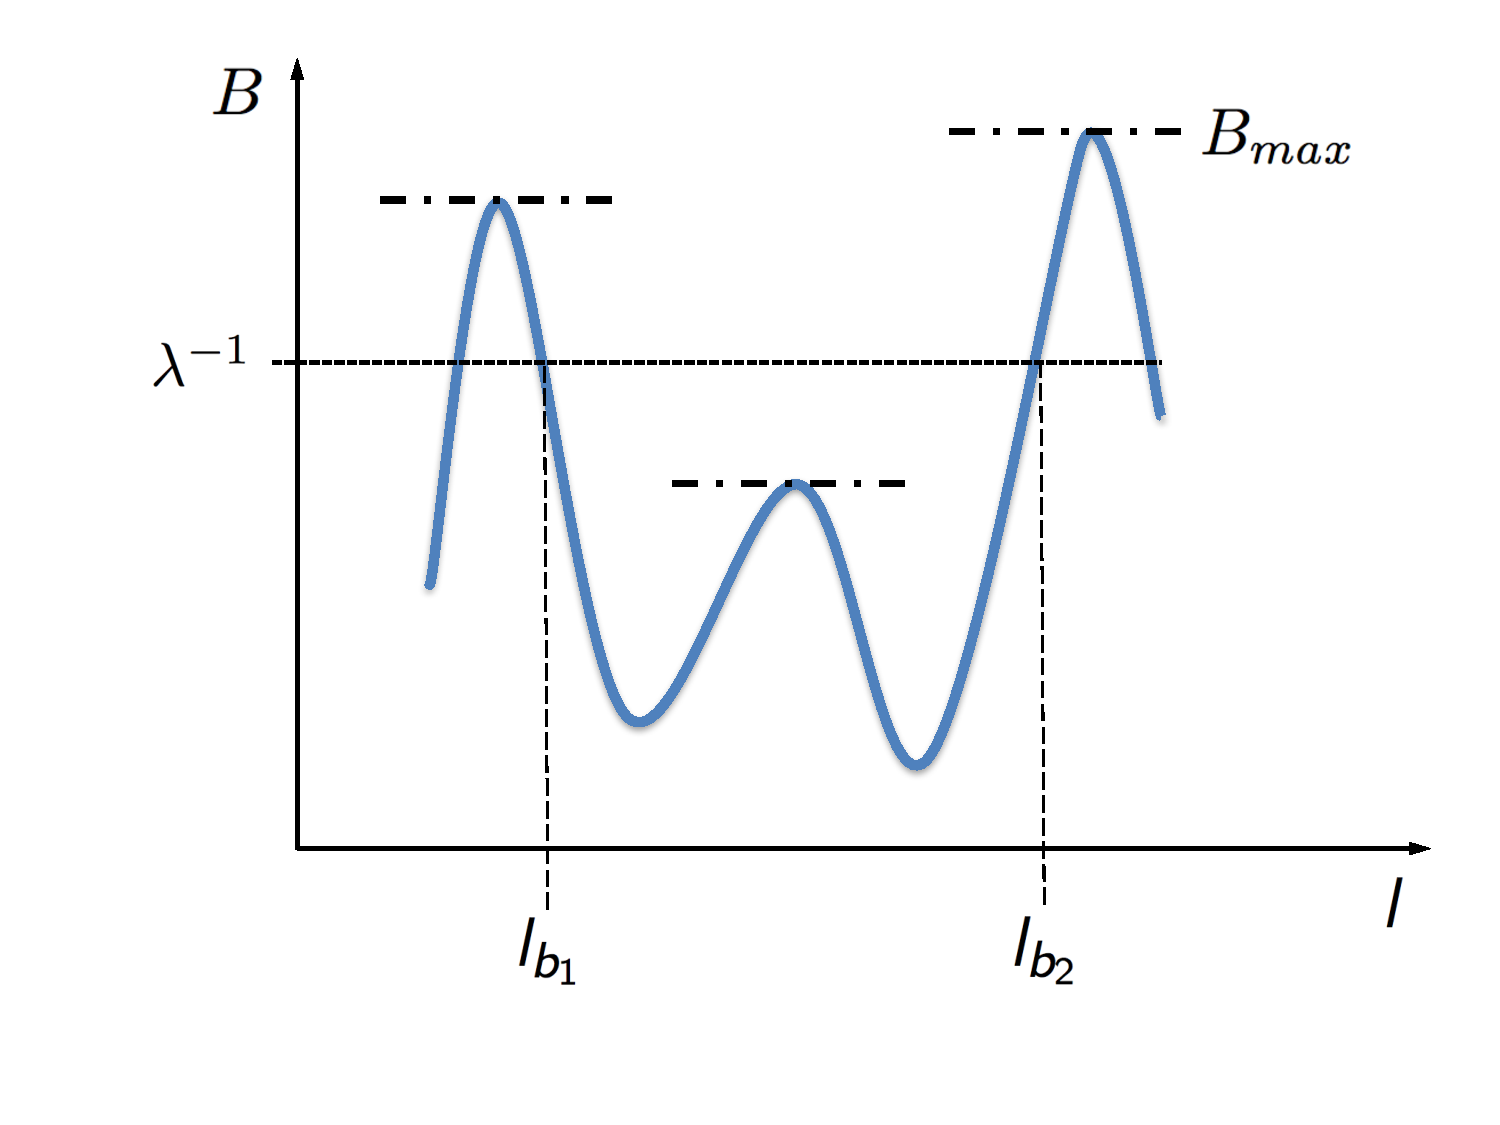
\includegraphics[angle=0,width=0.6\columnwidth]{figures/B_l}
\caption{Sketch of a particle trajectory at fixed $\alpha$. divergences are indicated with dot-dashed horizontal lines.}
\label{FIG_ORBIT}
\end{figure}

\KNOSOS~solves equations~(\ref{EQ_DKEFINAL}) and (\ref{EQ_QNFINAL}), together with equation~(\ref{EQ_AMB}). These equations have been rigorously derived in~\citep{calvo2018jpp} under the hypotheses of low collisionality, large aspect ratio and closeness to omnigeneity (we note that large aspect-ratio is a common characteristic of real stellarators~\citep{beidler2011icnts} while, as noted in the introduction, closeness to omnigeneity is a property sought in present and future devices). At low collisionalities, the motion of particles along the magnetic field is much faster than collisions, and the distribution function does not depend on the arc length $l$. Closeness to omnigeneity makes neoclassical transport describable by a radially-local equation for the deviation of the distribution function of trapped particles from a Maxwellian. In particular, it guarantees that the bounce-averaged radial drift is small enough so that
\begin{equation}
\left|\int_{l_{b_1}}^{l_{b_2}} \frac{\mathrm{d}l}{|v_\parallel|} \mathbf{v}_{D,b}\cdot\nabla\psi~\partial_\psi g_b\right|\ll
\left|\int_{l_{b_1}}^{l_{b_2}} \frac{\mathrm{d}l}{|v_\parallel|} \mathbf{v}_{D,b}\cdot\nabla\alpha~\partial_\alpha g_b\right|\,
\label{EQ_LOCAL}
\end{equation}
even in situations of small $E\times B$ drift. Hence, for stellarators close to omnigenity, terms proportional to $\partial_\psi g$ do not appear in equation~(\ref{EQ_DKEFINAL}). Finally, the large-aspect ratio approximation allows us to use the pitch-angle collision operator, equation~(\ref{EQ_COLOP}).
 
Let us finally discuss the neoclassical regimes that equations~(\ref{EQ_DKEFINAL}) and (\ref{EQ_QNFINAL}) can describe. The second term on the left-hand side of equation~(\ref{EQ_DKEFINAL}) includes the radial magnetic and $E\times B$ drifts caused by the inhomogeneity of the magnetic field strength and of the electrostatic potential on the flux surface, respectively. This means that equation~(\ref{EQ_DKEFINAL}) can model the $1/\nu$ regime and the transport caused by $\varphi_1$. The first term of the left-hand side includes the precession tangential to the flux surface caused by the radial variation of the electrostatic potential (i.e. the radial electric field $E_r$) and of the magnetic field strength. This implies that we can model the $\sqrt{\nu}$ and superbanana-plateau regimes. As discussed previously, radially global effects are not accounted for.






%\section{Details of the collision operator}\label{SEQ_COLOP}

%%%%%%%%%%%%%%%%%%%%%%%%%%%%%%%%%%%%%%%%%%%%%%%%%%%%%%%%%%%%%%%%%%%%%%%%%%%%%%%%%%%%%%%%%%%%%%%%%%%%%%%%%%%%%%%%%%%

%In this chapter, the pitch-angle-scattering collision operator has been employed, and its explicit expression has been provided in equation (\ref{EQ_COLOP}). As it has been discussed, this is a single-species collision operator, which is accurate for calculating ion transport, due to $\sqrt{m_e/m_i}\ll 1$. For electrons, however, electron-ion collisions need to be retained in the electron drift-kinetic equation. In order to overcome this limitation, an effective pitch-angle-scattering collsion frequency $\nu_{\lambda,b}$ is employed in order to account for inter-species collisions. This is done for both species, although its effect will be negligible for the ions.
%
%In this appendix, we provide the explicit expression of the pitch angle scattering frequency, given by the sum\footnote{We note that $\nu_{\lambda,b}=2\nu_b$, with the definition of $\nu_b$ of page 3 of~\cite{beidler2011icnts}.}
%\begin{equation}
%\nu_{\lambda,b}=\sum_{b'}\nu_0^{b/b'}\left[\mbox{erf} \left(\sqrt{m_{b'} v^2 /(2T_{b'})}\right) - \chi \left(\sqrt{m_{b'} v^2 /(2T_{b'})} \right)\right]\,,
%\end{equation}
%with
%\begin{equation}
%\nu_0^{b/b'}= \frac{8\pi  n_{b'} {Z_b}^2{Z_{b'}}^2  e^4 \ln \Lambda^{b/b'}}{m_b^2 v^3} \,.
%\end{equation}
%Here, $\ln \Lambda^{b/b'}$ is the Coulomb logarithm, 
%\begin{equation}
%\chi (x) = \frac{\mbox{erf} (x) - (2 x/\sqrt{\pi})\exp(-x^2)}{2x^2}\,,
%\end{equation}
%and
%\begin{equation}
%\mbox{erf}(x) = (2/\sqrt{\pi}) \int_0^x \exp (- t^2)\, \mathrm{d} t
%\end{equation}
%is the error function.


\chapter{Solution of the equations}\label{CHAP_SOL}

\footnote{This chapter corresponds to section 3 and appendices B and C of~\citep{velasco2019knosos}.}
In this chapter, we provide an overview of how equations~(\ref{EQ_DKEFINAL}) and (\ref{EQ_QNFINAL}) are solved. We first give an explicit expression for equation~(\ref{EQ_DKEFINAL}) in \S\ref{SEC_FINALDKE} and we discuss how to calculate its bounce-averaged coefficients in \S\ref{SEC_COEFFICIENTS}. We then devote \S\ref{SEC_GRID} to build the grid in which we will evaluate the distribution function, and \S\ref{SEC_SOLDKE} to discuss the discretization of the equation. Finally, the solution of quasineutrality, equation  (\ref{EQ_QNFINAL}), is addressed in \S\ref{SEC_SOLQN}.

\section{Final expression of the  drift-kinetic equation}\label{SEC_FINALDKE}

Using the expressions of the pitch-angle scattering collision operator described in equation~(\ref{EQ_COLOP}) and of the magnetic and $E\times B$ drifts in \textit{right handed} Boozer coordinates, equation~(\ref{EQ_DKEFINAL}) can be written in terms of a few bounce integrals:
\begin{eqnarray}
\left(I_{v_{M,\alpha}} (\alpha,\lambda)+\frac{1}{v_{d,b}}I_{v_E,\alpha}(\alpha,\lambda)\right)\partial_\alpha g_b &+& \left( I_{v_{M,\psi}}(\alpha,\lambda)+\frac{1}{v_{d,b}}I_{v_{E,\psi}}(\alpha,\lambda)\right) F_{M,b}\Upsilon_b\nonumber \\
&=& \frac{\nu_{\lambda,b}}{v_{d,b}} \partial_\lambda\left[ I_\nu(\alpha,\lambda) \partial_\lambda g_b\right]\,,
\label{EQ_NDKE}
\end{eqnarray}
with
\begin{eqnarray}
v_{d,b}&\equiv&\frac{m_bv^2}{Z_be}\,,\nonumber\\
I_{v_{E,\alpha}}&=&\Psi_t'\partial_\psi\varphi_0\int_{l_{b_1}}^{l_{b_2}} \frac{\mathrm{d}l}{\sqrt{1-\lambda B}}\,,\nonumber\\
I_{v_{M,\alpha}}&=&\int_{l_{b_1}}^{l_{b_2}}\frac{\mathrm{d}l }{\sqrt{1-\lambda B}}\left(1-\frac{\lambda B}{2}\right)\left[\Psi_t'\frac{\partial_\psi B}{B}+
 \frac{B_\zeta\partial_\theta B - B_\theta\partial_\zeta B}{B|B_\zeta+\iota B_\theta|}\zeta\partial_\psi \iota\right]\,,\nonumber\\
I_{v_{E,\psi}}&=&\int_{l_{b_1}}^{l_{b_2}} \frac{\mathrm{d}l}{\sqrt{1-\lambda B}}\frac{B_\theta\partial_\zeta \varphi_1 - B_\zeta\partial_\theta \varphi_1}{|B_\zeta+\iota B_\theta|}\,,\nonumber\\
I_{v_{M,\psi}}&=&\int_{l_{b_1}}^{l_{b_2}} \frac{\mathrm{d}l }{\sqrt{1-\lambda B}}\left(1-\frac{\lambda B}{2}\right)\frac{B_\theta\partial_\zeta B - B_\zeta\partial_\theta B}{B|B_\zeta+\iota B_\theta|}\,,\nonumber\\
I_\nu&=&\int_{l_{b_1}}^{l_{b_2}} \mathrm{d}l\frac{\lambda\sqrt{1-\lambda B}}{B}\,.
\label{EQ_BINT}
\end{eqnarray}
where $B_\psi$, $B_\theta$ and $B_\zeta$ are the covariant components of $\mathbf{B}$, and $B_\psi=0$ in the low-$\beta$ approximation. We note that only $v_{d,b}$, $\nu_{\lambda,b}$, $F_{M,b}$ and $\Upsilon_b$ depend on the species: the bounce-integrals are only determined by the magnetic configuration and the electrostatic potential. {The magnetic shear appears explicitly  in $I_{v_{M,\alpha}}$.}

Equation~(\ref{EQ_NDKE}) is a differential equation in two variables only, $\alpha$ and $\lambda$, which is the origin of the fast performance of~\KNOSOS~that will be demonstrated in chapter~\ref{CHAP_EX}. The radial coordinate $\psi$ is a parameter, since we are solving radially local equations; $v$ is a parameter as well, since $\varphi_1\ll \varphi_0$; and finally $l$ has disappeared since the coefficients are bounce-averages of certain quantities. The calculation of these coefficients is described in \S\ref{SEC_COEFFICIENTS}.

%%%%%%%%%%%%%%%%%%%%%%%%%%%%%%%%%%%%%%%%%%%%%%%%%%%%%%%%%%%%%%%%%%%%%%%%%%%%%%%%%%%%%%%%%%%%%%%%%%%%%%%%%%%%%%%%%%%

\section{Calculation of the coefficients of the drift-kinetic equation}\label{SEC_COEFFICIENTS}

%%%%%%%%%%%%%%%%%%%%%%%%%%%%%%%%%%%%%%%%%%%%%%%%%%%%%%%%%%%%%%%%%%%%%%%%%%%%%%%%%%%%%%%%%%%%%%%%%%%%%%%%%%%%%%%%%%%

The integrals in $l$ are done using an extended midpoint rule \citep[see e.g.][subroutine {\ttfamily midpnt}]{numericalrecipes}. This open formula is appropriate for integrals that are improper in the sense that they have an integrable singularity at the integration limits. This is our case, since by definition $\lambda B(l_{b_1}) = \lambda B(l_{b_2}) =1$. The number of points that we use is not pre-defined: starting from being one, it is tripled until the integral converges. %Specifically, until the relative variation of the numerical integral is smaller than \vlink{PREC\_BINT}.

Let us now note that integrals such as those of equations~(\ref{EQ_BINT}) may be difficult to converge if the numerator does not go to zero in the integration limits, or it does, but slower than the denominator. This may happen, first, if $\lambda$ is such that $l_{b_1}$ or $l_{b_2}$ are close to a point $l_T$ where $B(l)$ has a local maximum $B(l_T)$ for fixed $\alpha$; second, if the interval ($l_{b_1},l_{b_2}$) contains a point $l_B$ where $B(l)$ has a local maximum and $\lambda$ is close to $\lambda_B\equiv 1/B(l_B)$. In such cases, $I(\lambda)$ may become very large; if the inverse of $\lambda$  is equal to the corresponding maximum of $B$, the integral diverges logarithmically.  We can physically identify these situations in the example of figure~\ref{FIG_ORBIT}: divergences happen at \textit{bifurcations}, where orbits go from being trapped in a particular  region in $l$ to be trapped, for smaller $\lambda$, in a wider region (the boundary between passing and trapped particles is a particular case of this).  

One can ease the convergence, and thus make the calculation faster, by removing the divergence and solving it analytically as explained in Appendix C of~\citep{calvo2017sqrtnu}. This is described more in detail in the next subsection. Another subsection discusses how the fact that field lines are straight in magnetic coordinates is used to accelerate the evaluation of the magnetic field strength at each point ($\alpha, l$) without loss of accuracy.

%%%%%%%%%%%%%%%%%%%%%%%%%%%%%%%%%%%%%%%%%%%%%%%%%%%%%%%%%%%%%%%%%%%%%%%%%%%%%%%%%%%%%%%%%%%%%%%%%%%%%%%%%%%%%%%%%%%

\subsection{Analytical calculation of the divergences of some bounce-integrals}\label{SEC_DIV}

%%%%%%%%%%%%%%%%%%%%%%%%%%%%%%%%%%%%%%%%%%%%%%%%%%%%%%%%%%%%%%%%%%%%%%%%%%%%%%%%%%%%%%%%%%%%%%%%%%%%%%%%%%%%%%%%%%%

In this subsection, we discuss how integrals such as those in equations~(\ref{EQ_BINT}),
\begin{equation} 
I(\lambda)=\int_{l_{b_1}}^{l_{b_2}}\mathrm{d}l\,\frac{f(\lambda,l)}{\sqrt{1-\lambda B(l)}}\,,
\end{equation}
can be computed efficiently by removing the component that diverges close to bifurcations and solving it analytically. Since integration is done at fixed $\alpha$, we ease the notation by not making it explicit that $B$, $f$, and $I$ generally depend on the angular coordinate.
%can be computed efficiently by removing the component that diverges close to bifurcations and solving it analytically if \vlink{REMOVE\_DIV} is set to \true. Since integration is done at fixed $\alpha$, we ease the notation by not making it explicit that $B$, $f$, and $I$ generally depend on the angular coordinate.

We first expand the magnetic field around the bounce point:
\begin{equation} 
B(l)=B(l_{b_1})+\partial_l B|_{l_{b_1}}(l-l_{b_1})+\frac{1}{2}\partial^2_l B|_{l_{b_1}}(l-l_{b_1})^2\,.
\end{equation}
Close to the bounce point, we have
\begin{eqnarray}
\frac{f(l)}{\sqrt{1-\lambda B(l)}} \approx \frac{f(l_{b_1})}{\sqrt{-\lambda (l-l_{b_1}) [\partial_l B|_{l_{b_1}}+\frac{1}{2}\partial^2_l B|_{l_{b_1}}(l-l_{b_1})]}}\,
\end{eqnarray}
since $\lambda B(l_{b_1})=1$. We can proceed exactly in the same way close to $l_{b_2}$, and similarly close to $\lambda_B$: there, $\lambda B(l_B)<1$ and the first derivative $\partial_l B|_{l_B}$ is zero, and we have
\begin{eqnarray}
\frac{f(l)}{\sqrt{1-\lambda B(l)}} \approx \frac{f(l_B)}{\sqrt{-(\lambda-\lambda_B) B(l_B)-\lambda_B\frac{1}{2}\partial^2_l B|_{l_B}(l-l_B)^2}}\,.
\end{eqnarray}
We can then split the integral in three contributions:
\begin{equation} 
I= I_0+I_1+I_2+I_B\,,
\end{equation}
with
\begin{eqnarray}
I_0 &=&  \int_{l_{b_1}}^{l_{b_2}}\mathrm{d}l\,\left(\frac{f(l)}{\sqrt{1-\lambda B(l)}}\right.\nonumber\\
 &-&\frac{f(l_{b_1})}{\sqrt{-\lambda (l-l_{b_1}) [\partial_l B|_{l_{b_1}}+\frac{1}{2}\partial^2_l B|_{l_{b_1}}(l-l_{b_1})]}}\nonumber\\
 &-&\frac{f(l_{b_2})}{\sqrt{-\lambda (l-l_{b_2}) [\partial_l B|_{l_{b_2}}+\frac{1}{2}\partial^2_l B|_{l_{b_2}}(l-l_{b_2})]}}\nonumber\\
 &-&\left.\frac{f(l_B)}{\sqrt{-(\lambda-\lambda_B) B(l_B)-\lambda_B\frac{1}{2}\partial^2_l B|_{l_B}(l-l_B)^2}}\right)\,,
\end{eqnarray}
whose integrand does not diverge anywhere and
\begin{eqnarray} 
I_1 &=&  \int_{l_{b_1}}^{l_{b_2}}\mathrm{d}l\,\frac{f(l)}{\sqrt{-\lambda (l-l_{b_1}) [\partial_l B|_{l_{b_1}}+\frac{1}{2}\partial^2_l B|_{l_{b_1}}(l-l_{b_1})]}}\,,\nonumber\\
I_2 &=&  \int_{l_{b_1}}^{l_{b_2}}\mathrm{d}l\,\frac{f(l)}{\sqrt{-\lambda (l-l_{b_2}) [\partial_l B|_{l_{b_2}}+\frac{1}{2}\partial^2_l B|_{l_{b_2}}(l-l_{b_2})]}}\,,\nonumber\\
I_B &=&  \int_{l_{b_1}}^{l_{b_2}}\mathrm{d}l\,\frac{f(l_B)}{\sqrt{-(\lambda-\lambda_B) B(l_B)-\lambda_B\frac{1}{2}\partial^2_l B|_{l_B}(l-l_B)^2}}\,,
\end{eqnarray}
which can be solved analytically. The integral close to the bottom is
\begin{eqnarray} 
I_B &=&  \sqrt{\frac{-2}{\lambda_B\partial^2_l B|_{l_B}}} \left[\mathrm{ln}\left(x+\sqrt{x^2+\frac{2(\lambda-\lambda_B) B(l_B)}{\lambda_B\partial^2_l B|_{l_B}}}\right)\right]^{l_B-l_{b_1}}_0\nonumber\\
&+&  \sqrt{\frac{-2}{\lambda_B\partial^2_l B|_{l_B}}} \left[\mathrm{ln}\left(x+\sqrt{x^2+\frac{2(\lambda-\lambda_B) B(l_B)}{\lambda_B\partial^2_l B|_{l_B}}}\right)\right]_0^{l_{b_2}-l_B}\,.
\end{eqnarray}

For the other two integrals, if $\partial^2_l B|_{l_{b_1}}<0$ and $\partial^2_l B|_{l_{b_2}}<0$, the solution is
\begin{eqnarray} 
I_1 &=&  \sqrt{\frac{-2}{\lambda\partial^2_l B|_{l_{b_1}}}}  \times\nonumber\\
& &\hskip-0.5cm \left[\mathrm{ln}\left(2\lambda\sqrt{\frac{\partial^2_l B|_{l_{b_1}}}{-2}}\sqrt{ -\partial_l B|_{l_{b_1}}x -\frac{1}{2}\partial^2_l B|_{l_{b_1}}x^2} -\lambda \partial^2_l B|_{l_{b_1}} x -\lambda\partial_l B|_{l_{b_1}}\right)\right]_0^{l_{b_2}-l_{b_1}}\,,\nonumber\\
I_2 &=&  \sqrt{\frac{-2}{\lambda\partial^2_l B|_{l_{b_2}}}}  \times\nonumber\\
& &\hskip-0.5cm\left[\mathrm{ln}\left(2\lambda\sqrt{\frac{\partial^2_l B|_{l_{b_2}}}{-2}}\sqrt{ -\partial_l B|_{l_{b_2}}x -\frac{1}{2}\partial^2_l B|_{l_{b_2}}x^2} -\lambda \partial^2_l B|_{l_{b_2}} x -\lambda\partial_l B|_{l_{b_2}}\right)\right]_{l_{b_1}-l_{b_2}}^0\hskip-0.5cm.
\end{eqnarray} 
These expressions are useful (in the sense of removing large analytical contributions to $I$) close enough to a bifurcation, where they can significantly accelerate the convergence of equations~(\ref{EQ_BINT}), but they are in principle valid for any $\lambda$ (far from bifurcations,  when $\partial^2_l B|_{l_{b_1}}$ is positive, the expression within the square-root may become negative and cannot be used).

%Figure~\ref{FIG_INT} shows the integrands of $I$, $I_1$, $I_2$ and $I_B$ for one particular case of the calculation of the bounce-averaged coefficients of equation~(\ref{EQ_BINT}). It is shown that, by calculating anallitically $I_1$, $I_2$ and $I_B$. For values of $1/\lambda$ close enough to the corresponding maximum of $B$, the , the calculation of 
%It works better the more optimized the stellarator, as we learn from the figure: this particular orbit passes close not only to the relative maxima of $B$ corresponding to $\lambda_B$ but also close to other relative maxima that we ignore. In some cases, resolving numerically the large contribution of these maxima to the integral may get as computationally hard as the contributions that we have removed. These situations will be more frequent in the $\sqrt{\nu}$ regime (where the boundary layer between trapped and passing particles need to be well described~\citep{calvo2017sqrtnu}) than in the 1/$\nu$ or superbanana-plateau regimes.

%%%%%%%%%%%%%%%%%%%%%%%%%%%%%%%%%%%%%%%%%%%%%%%%%%%%%%%%%%%%%%%%%%%%%%%%%%%%%%%%%%%%%%%%%%%%%%%%%%%%%%%%%%%%%%%%%%%

\subsection{Evaluation of the magnetic field strength along a field line}\label{SEC_DELTA}

%%%%%%%%%%%%%%%%%%%%%%%%%%%%%%%%%%%%%%%%%%%%%%%%%%%%%%%%%%%%%%%%%%%%%%%%%%%%%%%%%%%%%%%%%%%%%%%%%%%%%%%%%%%%%%%%%%%

The fact that field lines are straight in magnetic coordinates can also be used to speed up the calculation of the coefficients of the drift-kinetic equation. We describe how in this subsection. 
%The fact that field lines are straight in magnetic coordinates can also be used to speed up the calculation of the coefficients of the drift-kinetic equation if \vlink{DELTA}  is set to \true. We describe how in this subsection. 

The bounce-integrals are done, using the algorithm mentioned in \S\ref{SEC_COEFFICIENTS}, by following field lines using a fixed step in the Boozer angles given by $\Delta\zeta$ and $\Delta\theta=\iota\Delta\zeta$. After each step, the magnetic field can be calculated without loss of accuracy from its Fourier components
\begin{eqnarray}
B(\theta,\zeta)&=&\sum_{m,n}  B_{m,n}^{(c)}(\cos[m\theta+nN\zeta]\nonumber\\
  &+&\sum_{m,n}  B_{m,n}^{(s)}(\cos[m\theta+nN\zeta]\,,\nonumber\\
B(\theta+\Delta\theta,\zeta+\Delta\zeta)&=&\sum_{m,n} B_{m,n}^{(c)}\cos[m(\theta+\Delta\theta)+nN(\zeta+\Delta\zeta)]\nonumber\\
&+&\sum_{m,n} B_{m,n}^{(s)}\sin[m(\theta+\Delta\theta)+nN(\zeta+\Delta\zeta)]\,,\nonumber\\
B(\theta+2\Delta\theta,\zeta+2\Delta\zeta)&=&\sum_{m,n} B_{m,n}^{(c)}\cos[m(\theta+2\Delta\theta)+nN(\zeta+2\Delta\zeta)]\nonumber\\
&+&\sum_{m,n} B_{m,n}^{(s)}\sin[m(\theta+2\Delta\theta)+nN(\zeta+2\Delta\zeta)]\,,\nonumber\\
...
\end{eqnarray}
Instead of calculating the cosines at every angular position, we can precalculate a few sines and cosines, $\cos(m\theta+nN\zeta)$, $\sin(m\theta+nN\zeta)$, $\cos(m\Delta\theta+nN\Delta\zeta)$ and $\sin(m\Delta\theta+nN\Delta\zeta)$, and use well-known trigonometric identities to iterate:
 \begin{eqnarray}
\cos[m(\theta+\Delta\theta)+nN(\zeta+\Delta\zeta)] & = &\cos(m\theta+nN\zeta)\cos(m\Delta\theta+nN\Delta\zeta)\nonumber\\
&-& sin(m\theta+nN\zeta)\sin(m\Delta\theta+nN\Delta\zeta)\,,\nonumber\\
\sin[m(\theta+\Delta\theta)+nN(\zeta+\Delta\zeta)] & =& \cos(m\theta+nN\zeta)\sin(m\Delta\theta+nN\Delta\zeta)\nonumber\\
&+& \sin(m\theta+nN\zeta)\cos(m\Delta\theta+nN\Delta\zeta)\,,
\end{eqnarray}
and
 \begin{eqnarray}
\cos[m(\theta+2\Delta\theta)+nN(\zeta+2\Delta\zeta)] & =& \cos[m(\theta+\Delta\theta)+nN(\zeta+\Delta\zeta)]\cos(m\Delta\theta+nN\Delta\zeta)\nonumber\\
&-& sin[m(\theta+\Delta\theta)+nN(\zeta+\Delta\zeta)]\sin(m\Delta\theta+nN\Delta\zeta)\,,\nonumber\\
\sin[m(\theta+2\Delta\theta)+nN(\zeta+2\Delta\zeta)] & = &\cos[m(\theta+\Delta\theta)+nN(\zeta+\Delta\zeta)]\sin(m\Delta\theta+nN\Delta\zeta)\nonumber\\
&+& \sin[m(\theta+\Delta\theta)+nN(\zeta+\Delta\zeta)]\cos(m\Delta\theta+nN\Delta\zeta)\,\nonumber\\
\end{eqnarray}
and so on.



%%%%%%%%%%%%%%%%%%%%%%%%%%%%%%%%%%%%%%%%%%%%%%%%%%%%%%%%%%%%%%%%%%%%%%%%%%%%%%%%%%%%%%%%%%%%%%%%%%%%%%%%%%%%%%%%%%%

\section{Spatial and velocity grid}\label{SEC_GRID}

%%%%%%%%%%%%%%%%%%%%%%%%%%%%%%%%%%%%%%%%%%%%%%%%%%%%%%%%%%%%%%%%%%%%%%%%%%%%%%%%%%%%%%%%%%%%%%%%%%%%%%%%%%%%%%%%%%%

In \S\ref{SEC_COEFFICIENTS} we have seen how the integrals of equations~(\ref{EQ_BINT}) are calculated. These integrals will be evaluated at the points ($\alpha,\lambda$) in which we want to determine the distribution function $g_b$. The selection of these points constitute the subject of this section.

Let us start with the spatial grid. We have seen that $\psi$ is a parameter, and $l$ does not appear in the bounce-averaged drift-kinetic equation, which leaves us with the field line label $\alpha$. There are, however, two complications: first, at a given $\alpha$ and $\lambda$, several wells may exist (in other words, several pairs of $l_{b_1}$ and $l_{b_2}$), which means that we need to use an integer label $w$ for them (as we will discuss more in detail in the following section). Second, even if $g_b$ does not depend on $l$, its integrals over velocities (needed e.g. to compute $\varphi_1$, see equation~(\ref{EQ_QNFINAL})) do, so we must define a two-dimensional angular grid. As a general rule, when doing so, we try to minimize the number of points at which $g_b$ needs to be solved, in order to save computing resources. With this in mind, we make use of periodicity and align the grid points with the field lines. The grid points are also aligned with $\zeta=0$.

\begin{figure}\vskip-1.5cm
\centerline{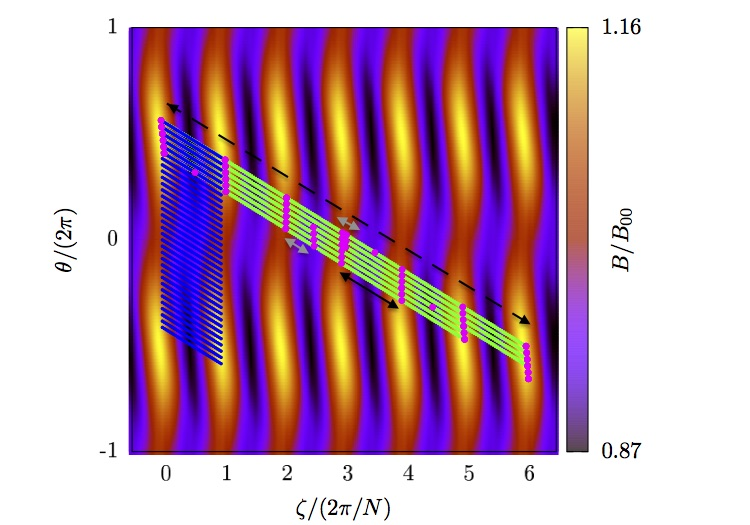
\includegraphics[angle=0,width=\columnwidth]{figures/ang_grid.jpg}}
\centerline{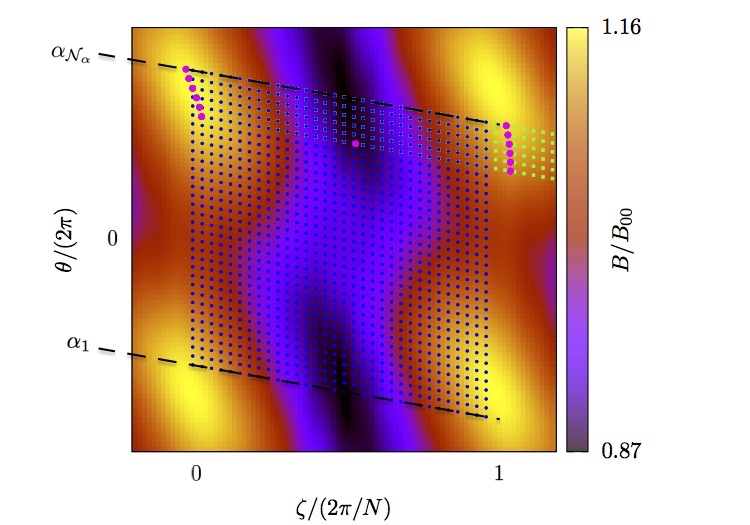
\includegraphics[angle=0,width=\columnwidth]{figures/ang_grid_zoom.jpg}}
\caption{Construction of the angular grid (see text) for a flux-surface of W7-X (top); zoom (bottom).}
\label{FIG_GRID}
\end{figure}

We use figure~\ref{FIG_GRID} (top), which shows one example of stellarator flux surface (the W7-X case discussed in \S\ref{SEC_DKES}) to describe how the angular grid is built. We follow several field lines until they have completed a full poloidal turn. The distance between two consecutive field lines $\Delta\alpha$ is taken to be an integer fraction (one sixth, in the plot) of $2\pi\iota/N$, where $N$ is the number of toroidal periods. This is how the green points are located, with uniform spacing in the toroidal angle. Along the field lines, several maxima of the magnetic field are found, plotted with magenta circles. It is observed that we are dealing with a relatively optimized configuration, in the sense that most trapped particles are so in a major well that coincides with one field period (black continuous arrow). In other words, their bounce points $l_{b_1}$ and $l_{b_2}$ are two consecutive magenta points, separated toroidally by a characteristic angular distance $\sim 2\pi/N$ (smaller for large values of $\lambda$, close to the bottom of the magnetic well). In the example, several ripple wells are found (grey arrows). For small enough values of $\lambda$, trajectories trapped in more than one field-period exist: in this example, particles may move between $\zeta=0$ and $\zeta=6\frac{2\pi}{N}$ (black dashed arrow); trajectories with smaller $\lambda$ (that is, trapped in more than 6 toroidal periods) are ignored in this case; this procedure effectively sets the boundary between passing and trapped particles (following field lines until they have completed more than one poloidal turn would allow us to describe trajectories with smaller $\lambda$,  but this is not necessary in the light of the results of chapter~\ref{CHAP_EX}).

Periodicity allows us to project all these grid points onto the first period. The result is a bidimensional grid in $\alpha$ and $l$, with ${\cal{N}}_\alpha$ and ${\cal{N}}_l$ points in each direction. ${\cal{N}}_\alpha$ is the integer quantity such that ${\cal{N}}_\alpha<\frac{2\pi}{\Delta\alpha}\le{\cal{N}}_\alpha+1$. The ${\cal{N}}_l$ points along the field line are distributed uniformly in the toroidal angle along a toroidal period, and ${\cal{N}}_l$ is the largest power of 2 that is smaller than or equal to ${\cal{N}}_\alpha$. This will be useful for a fast computation of the Fourier transform, needed when solving quasineutrality. Toroidal periodicity is also enforced at the corners of the grid: for instance, in figure~\ref{FIG_GRID} bottom, point $\alpha=\alpha_{{\cal{N}}_\alpha-4}$, $\zeta=0$, is not contained in the wells marked in magenta. Using periodicity, the value of the distribution function at  this point will be taken to be equal to the value at $\alpha=\alpha_1$ and $\zeta=2\pi/N$. The number of points where this has to be done can be minimized by putting one of the corners of the grid close to the global maximum of $B$ on the flux-surface. For each of the nodes of this grid (and for each of the possible values of $\lambda$) the points along the trajectory and the bounce points of particles trapped in one or several field-periods are now clearly identified, and the integrals of equation~(\ref{EQ_BINT}) can be evaluated. 

Let us turn our attention to the velocity grid, where we are using $\lambda$ and $v$ as coordinates. Since we have seen in chapter \ref{CHAP_EQ} that only trapped particles need to be calculated, an obvious choice for the former is a uniform grid\footnote{When the particles are in the $1/\nu$ regime, special attention should be paid to bifurcations, where $g_b$ has discontinuous first $\lambda$-derivatives~\citep{nemov1999neo,calvo2014er}, and a non-uniform grid, adapted to the structure of maxima and minima at fixed $\alpha$, is a more efficient choice~\citep{kernbichler2016neo2}. The same applies to very low collisionalities, when the contribution to the flux is concentrated on very thin $\lambda$ layers. For the wide parameter range that will be studied with~\KNOSOS, the uniform grid is considered appropriate.}, with ${\cal{N}}_\lambda+1$ values between $\lambda_1\equiv 1/B_{max}$ and $\lambda_{{\cal{N}}_\lambda+1}\equiv 1/B_{min}$. The distribution function will not be evaluated at $\lambda_{{\cal{N}}_\lambda+1}$, which will be \textit{ghost} points employed for imposing the boundary conditions at the bottom of the well. When integrating in $\lambda$, we will use the extended trapezoidal rule~\citep[][]{numericalrecipes}.

Finally, $v$ is a parameter in our calculations: equation~(\ref{EQ_NDKE}) will be solved for several values $v_i$ of the velocity and the solution will be numerically integrated in $v$. Since the integrand of equations~(\ref{EQ_VELINT}) contains an exponential coming from the Maxwellian distribution, we will use Gauss-Laguerre of order 64~\citep[][]{numericalrecipes}:
\begin{equation}
\int_0^\infty\,\mathrm{d}(v^2/v_{th,b}^2) f(v^2/v_{th,b}^2) \exp{(-v^2/v^2_{th,b})} \approx \sum_{i=1}^{n} \omega_i f(v_i^2/v_{th,b}^2)\,,
\label{EQ_CONV}
\end{equation}
being $v_{th,b}$ the thermal velocity of species $b$, and $\omega_i$ a set of tabulated real numbers. This procedure requires solving the monoenergetic drift-kinetic equation for $n=64$ values of $v/v_{th,b}$, typically from $\sim 10^{-2}$ to $\sim 10^2$. However, the contribution of the largest $v_i$ to the integral can be usually neglected, and this allows for an important reduction of computing time. Let us finally note that this is a standard and well-tested choice in neoclassics and gyrokinetics~\citep[e.g.][]{velasco2011bootstrap,barnes2019stella}, although other velocity-space discretization methods have been proposed in recent years~\citep{landreman2013intv} that could be easily implemented in~\KNOSOS.

%%%%%%%%%%%%%%%%%%%%%%%%%%%%%%%%%%%%%%%%%%%%%%%%%%%%%%%%%%%%%%%%%%%%%%%%%%%%%%%%%%%%%%%%%%%%%%%%%%%%%%%%%%%%%%%%%%%

\section{Discretization of the drift-kinetic equation}\label{SEC_SOLDKE}

%%%%%%%%%%%%%%%%%%%%%%%%%%%%%%%%%%%%%%%%%%%%%%%%%%%%%%%%%%%%%%%%%%%%%%%%%%%%%%%%%%%%%%%%%%%%%%%%%%%%%%%%%%%%%%%%%%%

In \S\ref{SEC_GRID} we have built a grid in variables $\alpha$ and $\lambda$. Three integers can be used to label any point $(\alpha_i,\lambda_j,w)$ of this grid: $i$ runs from 1 to  ${\cal{N}}_\alpha$,  $j$ from 1 to ${\cal{N}}_\lambda$ and $w=I,II...$ is an integer that labels wells for a given $\alpha$ and $\lambda$. At a given point, we define $g_{i,j,w}\equiv g_b(\alpha_i,\lambda_j,w)$,  $I_{\nu,i,j,w}\equiv I_\nu(\alpha_i,\lambda_j,w)$ and so on (in order to ease the notation, $g_{i,j,w}$ does not contain a species index). The final step in the discretization of the drift-kinetic equation is how we approximate the derivatives of $g_b$ of equation~(\ref{EQ_NDKE}) at each point of this grid.


Let us start with the collision operator, which divided by $ \frac{\nu_{\lambda},b}{v_{d,b}}$ reads
\begin{equation}
\partial_\lambda\left[ I_\nu \partial_\lambda g_b\right]\,,
\label{EQ_COL}
\end{equation}
and can be expanded into two terms
\begin{equation}
\left[ I_\nu \partial^2_\lambda  + (\partial_\lambda I_\nu) \partial_\lambda \right] g_b\,. 
\label{EQ_CO_EXP}
\end{equation}
We represent the $\lambda$ grid at fixed $\alpha$ in figure~\ref{FIG_LAMBDA}. Here, $\lambda_1$ is the boundary between passing and trapped particles. In this example, only one complete well is plotted at $\lambda_2$, labelled $I$. If one moves to larger $\lambda$, a bifurcation appears in the vicinity of $\lambda_{j_0}$, with two wells labelled $I$ and $II$. At a larger value of $\lambda$, there are the bottoms of the wells, where the wells have their minimum magnetic field (different in $I$ than in $II$) and beyond which no orbits are allowed.

 At a generic point, we make use of equation~(\ref{EQ_CO_EXP}) and then employ central finite differences with second-order accuracy
\begin{eqnarray}
\left[ I_\nu \partial^2_\lambda  + (\partial_\lambda I_\nu) \partial_\lambda \right] g_b|_{i,j,w}&=& I_\nu,_{i,j,w} \frac{g_{i,j+1,w}+g_{i,j-1,w}-2g_{i,j,w}}{(\Delta\lambda)^2}\nonumber\\&+&\partial_\lambda I_\nu |_{i,j,w} \frac{g_{i,j+1,w}-g_{i,j-1,w}}{2\Delta\lambda}\,,
\label{EQ_D2LAMBDA}
\end{eqnarray}
with $\Delta\lambda=\lambda_{j+1}-\lambda_j$. Differentiation is done at fixed $\alpha$ and well-label $w$. At a bifurcation, such as the one near $\lambda_{j_0}$ in figure~\ref{FIG_LAMBDA}, we use finite differences with second-order accuracy directly over equation~(\ref{EQ_COL}) and summing over wells,
%with $\Delta\lambda=\lambda_{j+1}-\lambda_j$. Differentiation is done at fixed $\alpha$ and well-label $w$. Nevertheless, equation~(\ref{EQ_D2LAMBDA}) relies on $\partial_\lambda g$ being continuous, which is not fulfilled at bifurcations if the effect of the tangential drift is small. At a bifurcation, such as the one near $\lambda_{j_0}$ in figure~\ref{FIG_LAMBDA}, we use finite differences with second-order accuracy directly over equation~(\ref{EQ_COL}) and summing over wells, 
\begin{eqnarray}
\partial_\lambda\left[ I_\nu \partial_\lambda g_b\right]|_{i,j_0,I}&=& \frac{[I_\nu \partial_\lambda g_b]|_{i,j_0+1,I} +  [I_\nu \partial_\lambda g_b]|_{i,j_0+1,II} -   [I_\nu \partial_\lambda g_b]|_{i,j_0-1,I}}{2\Delta\lambda}\,\nonumber\\
&=& I_\nu,_{i,j_0+1,I}\frac{g_{i,j_0+2,I}-g_{i,j_0,I}}{4(\Delta\lambda)^2}\nonumber\\
&+& I_\nu,_{i,j_0+1,II}\frac{g_{i,j_0+2,II}-g_{i,j_0,I}}{4(\Delta\lambda)^2}\nonumber\\
&-&I_\nu,_{i,j_0-1,I}\frac{g_{i,j_0,I}-g_{i,j_0-2,I}}{4(\Delta\lambda)^2}\,.\label{EQ_DLAMBDABIF}
\end{eqnarray}
This discretization is designed to obtain the expected relation between different values of $\partial_\lambda g$ at the bifurcation for the $1/\nu$ regime~\citep{nemov1999neo,calvo2014er}. Finally, we have two kinds of boundary conditions: one at the boundary between passing and trapped particles, corresponding to equation~(\ref{EQ_CONT2}),
\begin{equation}
g_{i,1,w}=0\,,
\label{EQ_TOP}
\end{equation}
and one at the bottom, corresponding to regularity~\citep{calvo2013er},
\begin{equation}
\partial_\lambda\left[ I_\nu \partial_\lambda g_b\right]|_{i,{\cal{N}}_\lambda,w} = -I_\nu,_{i,{\cal{N}_\lambda}-1,w}\frac{g_{i,{\cal{N}}_\lambda,w}-g_{i,{\cal{N}}_\lambda-2,w}}{4(\Delta\lambda)^2}\,.
\label{EQ_BOTTOM}
\end{equation}
Here we have employed a ghost point $\lambda_{{\cal{N}}_\lambda+1}$ at exactly the bottom of the well, where $I_{\nu,i,{\cal{N}}_\lambda+1,w}=0$. One precision must be made: while in omnigenous magnetic fields the values of the maxima and minima of $B$ are the same when moving in $\alpha$, and equation~(\ref{EQ_BOTTOM}) can be used as such for all $\alpha$, this ceases to be true in a generic stellarator. For instance, the distance from $\lambda_{{\cal{N}_\lambda}}$ to the local bottom will be exactly $\Delta\lambda$ for one field line and smaller elsewhere (it may even happen that the contour condition must not be applied to $\partial_\lambda\left[ I_\nu \partial_\lambda g_b\right]|_{i,{\cal{N}}_\lambda,w}$, but to $\partial_\lambda\left[ I_\nu \partial_\lambda g_b\right]|_{i,j,w}$ with a smaller $j$). This requires introducing straightforward corrections to equations~(\ref{EQ_D2LAMBDA}), (\ref{EQ_DLAMBDABIF}), (\ref{EQ_TOP}) and (\ref{EQ_BOTTOM}).

\begin{figure}
\centering
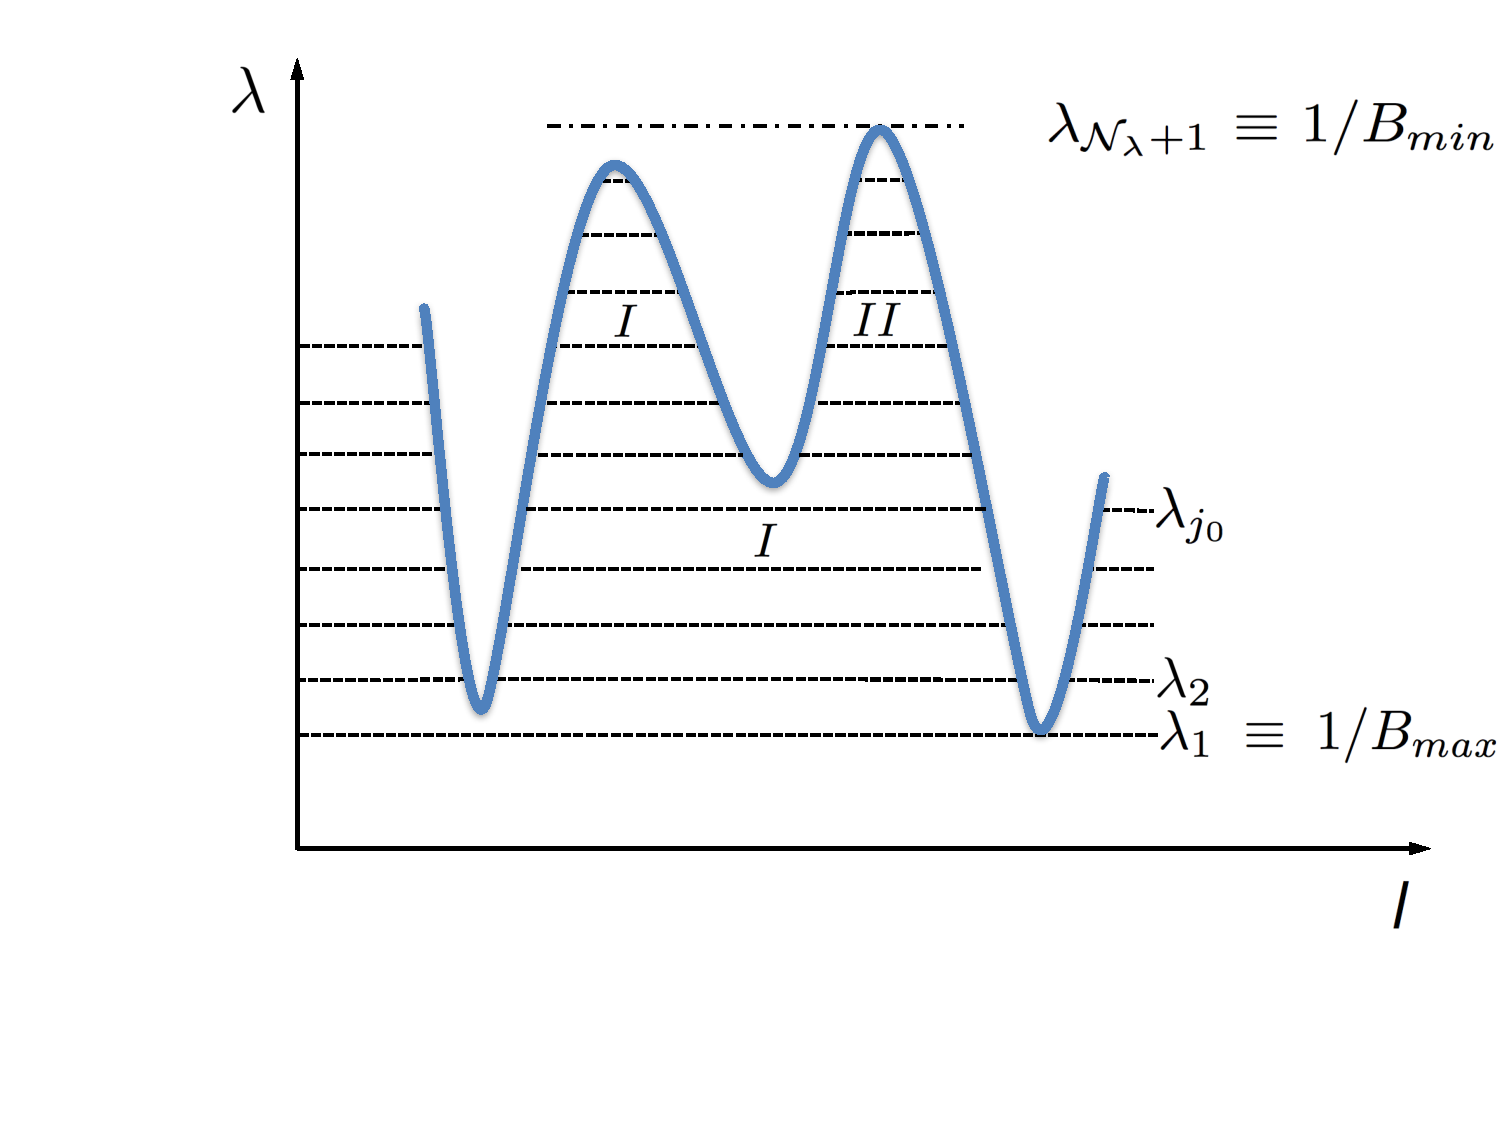
\includegraphics[angle=0,width=0.8\columnwidth]{figures/lambda_l}\
\caption{Sketch of grid in $\lambda$ space at fixed $\alpha$. The collision operator is discretized as in equation~(\ref{EQ_D2LAMBDA}) except at the top ($\lambda_1$) or bottom ($\lambda_{{\cal{N}}_\lambda}$) of the well and at bifurcations (e.g. $\lambda_{j_0}$); there, equations~(\ref{EQ_BOTTOM}),~(\ref{EQ_TOP})  and~(\ref{EQ_DLAMBDABIF}), respectively are used instead.}
\label{FIG_LAMBDA}
\end{figure}

\begin{figure}
\centering
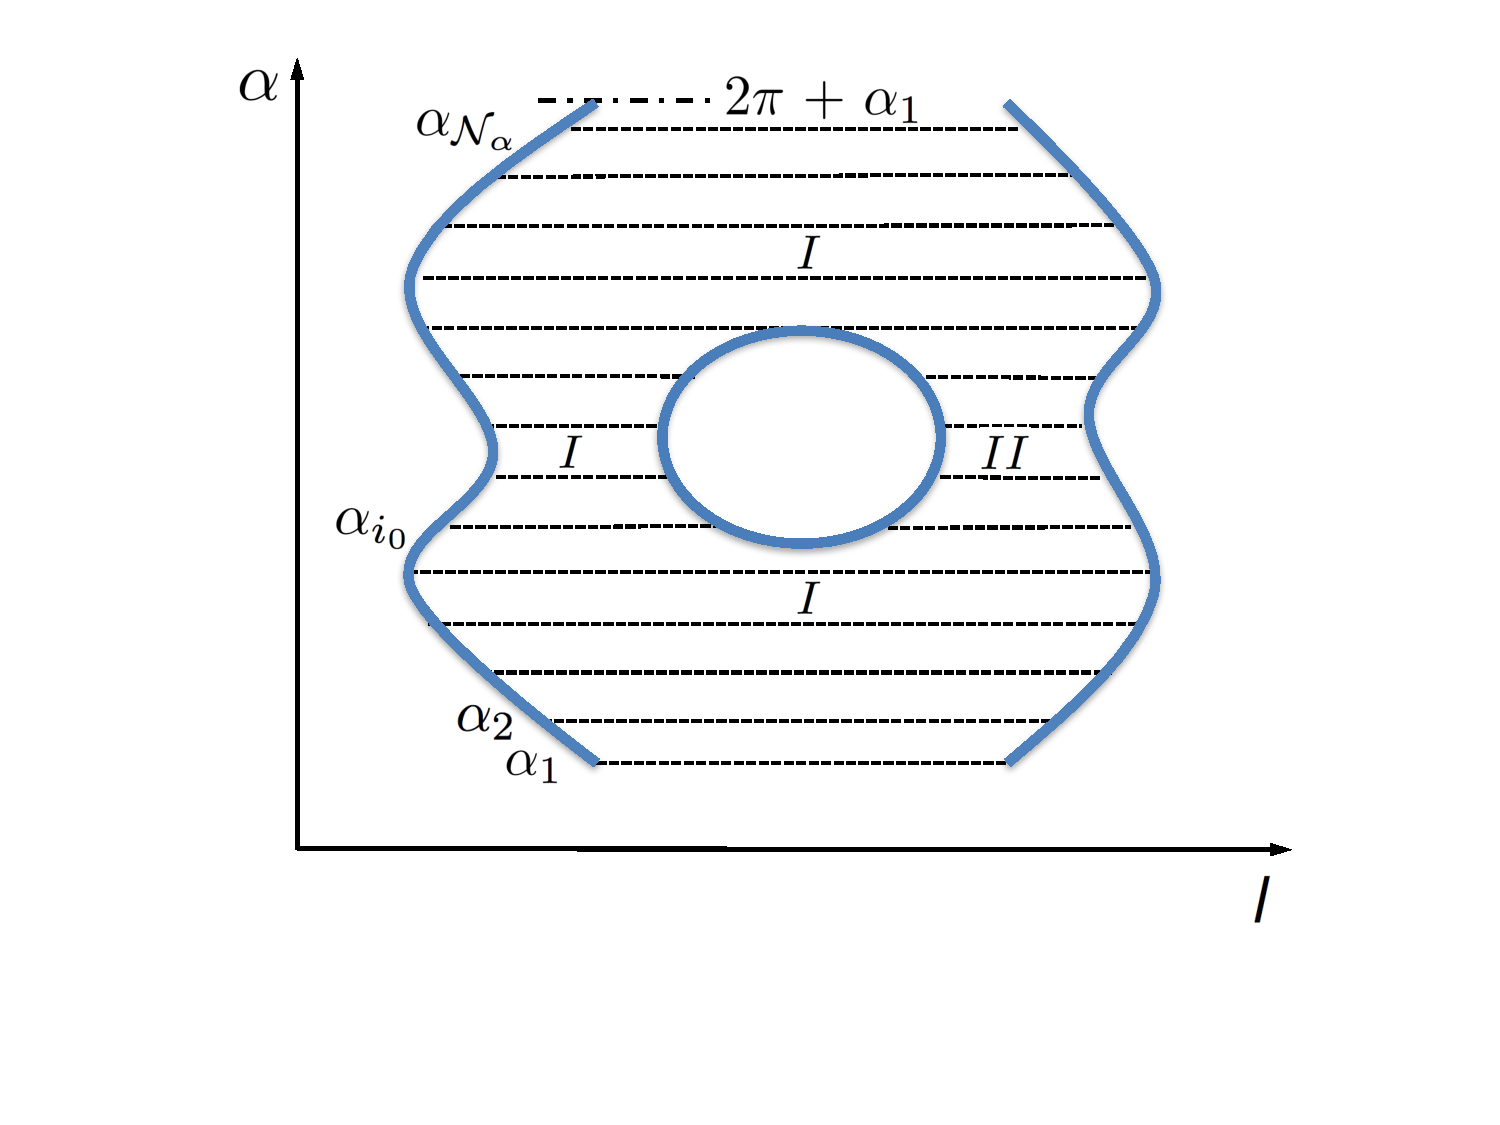
\includegraphics[angle=0,width=0.8\columnwidth]{figures/alpha_l}\vskip-1.5cm
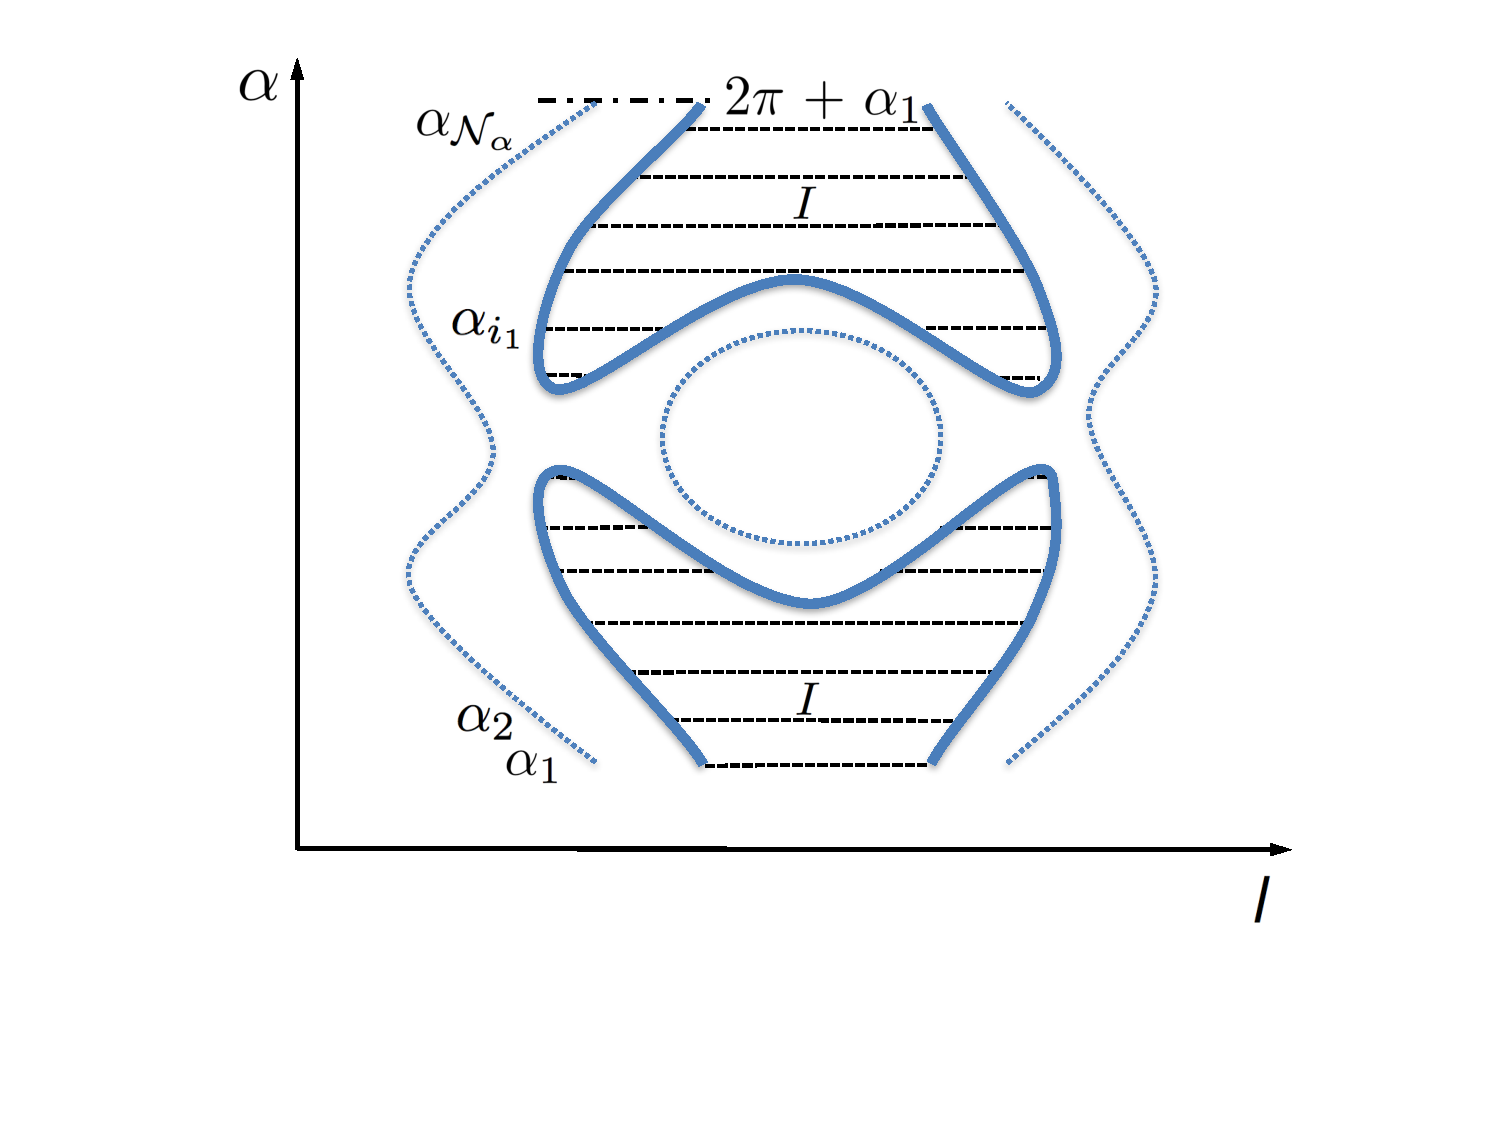
\includegraphics[angle=0,width=0.8\columnwidth]{figures/alpha_l_largelambda}\vskip-0.5cm
\caption{Top: sketch of grid in $\alpha$ space at fixed $\lambda$. The tangential derivatives are discretized as in equations~(\ref{EQ_FDALPHA}) and (\ref{EQ_BDALPHA}) except close to the limits of the grid ($\alpha_1$ and $\alpha_{{\cal{N}}_\alpha}$) and to bifurcations (e.g. $\alpha_{i_0}$); there, equations~(\ref{EQ_FDALPHAA}),~(\ref{EQ_FDALPHAB}),~(\ref{EQ_BDALPHAA}),~(\ref{EQ_BDALPHAB})  and~(\ref{EQ_BIFALPHA}) are used instead. Bottom:  sketch of grid in $\alpha$ space at larger $\lambda$ (the grid at smaller $\lambda$ is plotted for reference in dashed thin blue line). $\alpha_{i_1}$} is a point where the backward derivative is discretized as discussed in equation~(\ref{EQ_NOALPHA}).
\label{FIG_ALPHA}
\end{figure}

Let us now turn our attention to the terms with the first derivative in $\alpha$ in equation~(\ref{EQ_NDKE}), which we multiply by $v_{d,b}$:
\begin{equation}
\left(v_{d,b}I_{v_{M,\alpha}} +I_{v_E,\alpha}\right)\partial_\alpha g_b\,. 
\label{EQ_DALPHA}
\end{equation}
We represent the $\alpha$ grid at fixed $\lambda$ in figure~\ref{FIG_ALPHA} (top). In this example, there is only one well at $\alpha_1$, labelled $I$. If one moves from smaller to larger $\alpha$, a bifurcation appears in the vicinity of $\alpha_{i_0}$, with two wells labelled $I$ and $II$. At a larger value of $\alpha$, the wells merge into a single region labelled again $I$. The last point of the grid, $\alpha_{{\cal{N}}_\alpha}$, is close to $\alpha_1+2\pi$.

Non-centered finite differences with second-order accuracy are used. For a given flux-surface, for each solution of the drift-kinetic equation, the sign of the coefficient in front of $\partial_\alpha g_b$ (i.e. the direction of the flow in the $\alpha$ direction) indicates whether forward
\begin{equation}
\partial_\alpha g_b|_{i,j,w}=\frac{-g_{i+2,j,w}+4g_{i+1,j,w}-3g_{i,j,w}}{2\Delta\alpha}\,,
\label{EQ_FDALPHA}
\end{equation}
 or backward differences 
 \begin{equation}
\partial_\alpha g_b|_{i,j,w}=\frac{g_{i-2,j,w}-4g_{i-1,j,w}+3g_{i,j,w}}{2\Delta\alpha}\,,
\label{EQ_BDALPHA}
\end{equation}
should be used, with $\Delta\alpha=\alpha_{i+1}-\alpha_i$. To construct the derivatives with respect to $\alpha$ without much computational cost, we discretize separately the terms $I_{v_E,\alpha}\partial_\alpha g$ and $v_{d,b}I_{v_M,\alpha}\partial_\alpha g$ using a total of four matrices for a given flux surface. One corresponds to forward differences being used everywhere, and another one corresponds to backward differences everywhere. When solving equation ~(\ref{EQ_NDKE}), one of these two matrices will describe the $I_{v_E,\alpha}\partial_\alpha g$ term, depending on the sign of $E_r$. The other two matrices correspond to two $\lambda$ (and $w$)-dependent discretizations, in which forward (backward) differences are used according to the sign of $I_{v_{M,\alpha}}$. One of these two matrices will describe the $v_{d,b}I_{v_M,\alpha}\partial_\alpha g$ term, depending on the sign of $v_{d,b}$. Any matrix appropriate for describing equation~(\ref{EQ_DALPHA}) will thus be a linear combination of two of the four pre-calculated matrices, and a neoclassical simulation including ions and electrons and/or different values of the radial electric field will generally make use of the four of them.

Periodicity in $\alpha$ is easily imposed by replacing equation (\ref{EQ_FDALPHA}) at $i\ge{\cal{N}}_\alpha-1$ with
\begin{eqnarray}
\partial_\alpha g_b|_{{\cal{N}}_\alpha-1,j,w}&=&\frac{(g_{{\cal{N}}_\alpha,j,w}-g_{{\cal{N}}_\alpha-1,j,w})(2\pi+\alpha_1-\alpha_{{\cal{N}}_\alpha-1})}{(2\pi+\alpha_1-\alpha_{{\cal{N}}_\alpha})\Delta\alpha} \nonumber \\
&-&\frac{(g_{1,j,w}-g_{{\cal{N}}_\alpha-1,j,w})\Delta\alpha}{(2\pi+\alpha_1-\alpha_{{\cal{N}}_\alpha-1})(2\pi+\alpha_1-\alpha_{{\cal{N}}_\alpha})}\,,\label{EQ_FDALPHAA}\\
\partial_\alpha g_b|_{{\cal{N}}_\alpha,j,w}&=&\frac{(g_{1,j,w}-g_{{\cal{N}}_\alpha,j,w})(2\pi+\alpha_{2}-\alpha_{{\cal{N}}_\alpha})}{(2\pi+\alpha_{1}-\alpha_{{\cal{N}}_\alpha})\Delta\alpha} \nonumber \\
&-&\frac{(g_{2,j,w}-g_{{\cal{N}}_\alpha,j,w})(2\pi+\alpha_{1}-\alpha_{{\cal{N}}_\alpha})}{(2\pi+\alpha_{i}-\alpha_{{\cal{N}}_\alpha})\Delta\alpha}\,,\label{EQ_FDALPHAB}
\end{eqnarray}
respectively, and equation (\ref{EQ_BDALPHA}) at $i\le 2$ with
\begin{eqnarray}
\partial_\alpha g_b|_{2,j,w}&=&-\frac{(g_{1,j,w}-g_{2,j,w})(\alpha_{{\cal{N}}_\alpha}-\alpha_2-2\pi)}{(\alpha_{{\cal{N}}_\alpha}-\alpha_1-2\pi)\Delta\alpha} \nonumber \\
&+&\frac{(g_{{\cal{N}}_\alpha,j,w}-g_{2,j,w})\Delta\alpha}{(\alpha_{{\cal{N}}_\alpha}-\alpha_2-2\pi)(\alpha_{{\cal{N}}_\alpha}-\alpha_1-2\pi)}\,,\label{EQ_BDALPHAA}\\
\partial_\alpha g_b|_{1,j,w}&=&-\frac{(g_{{\cal{N}}_\alpha,j,w}-g_{1,j,w})(\alpha_{{\cal{N}}_\alpha-1}-\alpha_1-2\pi)}{(\alpha_{{\cal{N}}_\alpha}-\alpha_1-2\pi)\Delta\alpha} \nonumber \\
&+&\frac{(g_{{\cal{N}}_\alpha-1,j,w}-g_{1,j,w})(\alpha_{{\cal{N}}_\alpha}-\alpha_1-2\pi)}{(\alpha_{{\cal{N}}_\alpha-1}-\alpha_1-2\pi)\Delta\alpha}\,,
\label{EQ_BDALPHAB}
\end{eqnarray}
respectively. We note  that, since $\iota$ is generally irrational, $2\pi+\alpha_1-\alpha_{{\cal{N}}_\alpha}$ will e.g. be slightly smaller than $\Delta\alpha$


We also note that bifurcations do not pose a problem for $\alpha$-derivatives, due to $g_b$ being continuous in $\alpha$. For example, in the vicinity of $\alpha_{i_0}$ in figure~\ref{FIG_ALPHA} (top) the forward derivative is discretized
\begin{eqnarray}
\partial_\alpha g_b|_{i_0-2,j,I}&=&\frac{-g_{i_0-2,j,I}+4g_{i_0-1,j,I}-3g_{i_0,j,I}}{2\Delta\alpha}\nonumber\\
&=&\frac{-g_{i_0-2,j,I}+4g_{i_0-1,j,I}-3g_{i_0,j,II}}{2\Delta\alpha}\,,\nonumber\\
\partial_\alpha g_b|_{i_0-1,j,I}&=&\frac{-g_{i_0-1,j,I}+4g_{i_0,j,I}-3g_{i_0+1,j,I}}{2\Delta\alpha}\nonumber\\
&=&\frac{-g_{i_0-1,j,I}+4g_{i_0,j,II}-3g_{i_0+1,j,II}}{2\Delta\alpha}\,,\nonumber\\
\partial_\alpha g_b|_{i_0,j,I}&=&\frac{-g_{i_0,j,I}+4g_{i_0+1,j,I}-3g_{i_0+2,j,I}}{2\Delta\alpha}\,,\nonumber\\
\partial_\alpha g_b|_{i_0,j,II}&=&\frac{-g_{i_0,j,II}+4g_{i_0+1,j,II}-3g_{i_0+2,j,II}}{2\Delta\alpha}\,,\nonumber\\
\partial_\alpha g_b|_{i_0+1,j,I}&=&\frac{-g_{i_0+1,j,I}+4g_{i_0+2,j,I}-3g_{i_0+3,j,I}}{2\Delta\alpha}\,,\nonumber\\
\partial_\alpha g_b|_{i_0+1,j,II}&=&\frac{-g_{i_0+1,j,II}+4g_{i_0+2,j,II}-3g_{i_0+3,j,II}}{2\Delta\alpha}\,,\nonumber\\
\partial_\alpha g_b|_{i_0+2,j,I}&=&\frac{-g_{i_0+2,j,I}+4g_{i_0+3,j,I}-3g_{i_0+4,j,I}}{2\Delta\alpha}\,,\nonumber\\
\partial_\alpha g_b|_{i_0+2,j,II}&=&\frac{-g_{i_0+2,j,II}+4g_{i_0+3,j,II}-3g_{i_0+4,j,I}}{2\Delta\alpha}\,,\nonumber\\
\partial_\alpha g_b|_{i_0+3,j,I}&=&\frac{-g_{i_0+3,j,I}+4g_{i_0+4,j,I}-3g_{i_0+5,j,I}}{2\Delta\alpha}\,,\nonumber\\
\partial_\alpha g_b|_{i_0+3,j,II}&=&\frac{-g_{i_0+3,j,II}+4g_{i_0+4,j,I}-3g_{i_0+5,j,I}}{2\Delta\alpha}\,,
\label{EQ_BIFALPHA}
\end{eqnarray}
where continuity of $g_b$ has been used in the first two expressions of equation~(\ref{EQ_BIFALPHA}). Equivalent expressions can be obtained for the backward derivative.

One final caveat has to be made. In an omnigenous magnetic field, the contours of minimum $B$ on a flux surface must encircle the plasma (toroidally, poloidally, or helically). This is not true for a generic stellarator, in which local minima of $B$ exist on the flux surface. Close to these minima, moving in $\alpha$ at constant large $\lambda$ is not always possible, as these trajectories may not exist. This situation is illustrated in figure~\ref{FIG_ALPHA} (bottom), at $\alpha_{i_1}$. At, $\alpha_{i_1}$, instead of equation (\ref{EQ_BDALPHA}), we use
 \begin{equation}
\partial_\alpha g_b|_{i_1,j,w}=\frac{g_{i_1-2,j_0,w}-4g_{i_1-1,j,w}+3g_{i_1,j,w}}{2\Delta\alpha}\,.\label{EQ_NOALPHA}
\end{equation}
and we have implemented two models: in one, $\lambda_{j_0}$ is the value of $\lambda$ closest to $\lambda_j$ in which trajectories exist for all $\alpha$; in the second model, $\lambda_{j_0}$ is the closest value of $\lambda$ in which trajectories exist at $\alpha_{i_0-2}$. The relative differences between the two models are smaller than e.g. the error bars of~\DKES~in figure~\ref{FIG_D11PROF}. We note that (with different manifestations for other choices of velocity coordinates) an incorrect treatment of this kind of particles is common to all existing radially local codes.
%
%\
%
%~~~~~~~~~~~~~~~$\left(I_{v_{M,\alpha}}+\frac{1}{v_{d,b}}I_{v_{E,\alpha}}\right)\partial_\alpha +\frac{\nu_{\lambda,b}}{v_{d,b}} \partial_\lambda \nu\partial_\lambda $~~~~~~~~~$g_b$~~~~~~~$\left[I_{v_{M,\psi}} \right.+\left.\frac{1}{v_{d,b}}I_{v_{E,\psi}}\right] F_{M,b}\Upsilon_b$
%
%
%\[
%\begin{bmatrix}
%    \dots       & \dots & \dots & \dots &\dots \\
%    \dots       & \dots & \dots & \dots & \dots \\
%    \dots       & \dots & \dots & \dots & \dots \\
%    \dots       & \dots & \dots & \dots & \dots     
%\end{bmatrix}
%\cdot
%\begin{bmatrix}
%    \dots  \\
%    \dots  \\
%    \dots  \\
%    \dots 
%\end{bmatrix}
%=
%\begin{bmatrix}
%    \dots  \\
%    \dots  \\
%    \dots  \\
%    \dots 
%\end{bmatrix}
%\]
%
%\


For each of the species $b$, we end up with an equation that is linear in $g_b$ and can be written as a linear problem in matrix form. The matrix that represents
\begin{equation}
\left(I_{v_{M,\alpha}}+\frac{1}{v_{d,b}}I_{v_{E,\alpha}}\right)\partial_\alpha +\frac{\nu_{\lambda,b}}{v_{d,b}} \partial_\lambda \nu\partial_\lambda 
\end{equation}
is square with approximately ${\cal{N}}_\lambda\times {\cal{N}}_\alpha$ elements per row, and sparse, with $\sim 6$ non-zero elements per row: between 3 and 5 for the $\alpha$ derivatives, and typically 2 additional points for the collision operator. Although their relative weight varies with $\nu_{\lambda,b}$, $v_{d,b}$ and $\partial_\psi\varphi_0$, the non-zero elements are always at the same position for a given flux-surface, which can be used to save computing time, by using the four pre-computed matrices described above.

We solve the linear problem with a direct solver from the {\ttfamily PETSc} library~\citep{petsc-efficient,petsc-web-page,petsc-user-ref} based on LU factorization. The reason is that the matrix is not large enough to require iterative methods, and reusing the LU factorization greatly accelerates the solution of the quasineutrality equation, as discussed in \S\ref{SEC_SOLQN}.

%%%%%%%%%%%%%%%%%%%%%%%%%%%%%%%%%%%%%%%%%%%%%%%%%%%%%%%%%%%%%%%%%%%%%%%%%%%%%%%%%%%%%%%%%%%%%%%%%%%%%%%%%%%%%%%%%%%

\section{Solution of the quasineutrality equation}\label{SEC_SOLQN}

%%%%%%%%%%%%%%%%%%%%%%%%%%%%%%%%%%%%%%%%%%%%%%%%%%%%%%%%%%%%%%%%%%%%%%%%%%%%%%%%%%%%%%%%%%%%%%%%%%%%%%%%%%%%%%%%%%%

We will solve the quasineutrality equation by means of a response matrix approach (similar methods are used in gyrokinetics for the calculation of the electrostatic potential fluctuations~\citep{kotschenreuther1995response}). Let us first rewrite equations (\ref{EQ_NDKE}) and~(\ref{EQ_QNFINAL}) making explicit the dependence on $\varphi_1$:

\begin{eqnarray}
\left(I_{v_{M,\alpha}} +\frac{I_{v_{E,\alpha}}}{v_{d,b}}\right)\partial_\alpha g_b-\frac{\nu_{\lambda,b}}{v_{d,b}} \partial_\lambda I_\nu \partial_\lambda g_b ~~~~~~~~~~~~~~~~~~~~~~~~~~~~~~~~~~~& &\nonumber\\=\left(I_{v_{M,\psi}}-\int_{l_{b_1}}^{l_{b_2}} \frac{\mathrm{d}l}{\sqrt{1-\lambda B}}\frac{B_\theta\partial_\zeta \varphi_1 - B_\zeta\partial_\theta \varphi_1}{|B_\zeta+\iota B_\theta|} \right) F_{M,b}\Upsilon_b\,,\label{EQ_DKEPHI1}\\
\left(\frac{Z_i}{T_i}+\frac{1}{T_e}\right)\varphi_1 =\frac{2\pi}{en_e}\sum_b Z_b \int_0^\infty\mathrm{d} v \int_{B^{-1}_{{\rm max}}}^{B^{-1}}\mathrm{d}\lambda\frac{v^3 B}{|v_\parallel |}g_b\,.~~~~~~~~~~~~~~~\label{EQ_QNPHI1}
\end{eqnarray}
It can be observed that equation~(\ref{EQ_DKEPHI1}) is linear in $\varphi_1$, and therefore the response of the distribution function $g_b$ (and of its velocity integral) of species $b$ to certain $\varphi_1$ can be calculated as a superposition of the responses to a complete set of harmonics that parametrize $\varphi_1(\theta,\zeta)$. We can perform this parametrization efficiently thanks to the Fast Fourier Transform, using ${\cal{N}}=2(2{\cal{N}}_n+1)({\cal{N}}_m+1)$ coefficients:
\begin{equation}
\varphi_1(\theta,\zeta) =\sum_{-{\cal{N}}_n<n<{\cal{N}}_n} \sum_{0<m<{\cal{N}}_m} \left(\varphi^{(c)}_{mn}\cos(m\theta+Nn\zeta)+\varphi^{(s)}_{mn}\sin(m\theta+Nn\zeta)\right)\,
\label{EQ_FFTPHI1}
\end{equation}
(the grid defined in \S\ref{SEC_GRID} is not uniform in $\theta$, so an interpolation is done before the Fourier transform). We can now denote $u_k(\theta,\zeta)$ each of the ${\cal{N}}$ basis elements (e.g. $\cos(\theta+2N\zeta)$) and the combined system of drift-kinetic and quasineutrality equation can be symbolically written as
\begin{eqnarray}
\pmb{\varphi_1} = \pmb{\varphi_1^{0}} + \mathbf{A}\pmb{\varphi_1}\,,
\end{eqnarray}
where $\pmb{\varphi_1}$ is a vector whose ${\cal{N}}$ components are the coefficients of the expansion of $\varphi_1$ in equation~(\ref{EQ_FFTPHI1}) and $\mathbf{A}$ is a generally dense ${\cal{N}}\times{\cal{N}}$ matrix. In this linear, system, the right-hand side $\pmb{\varphi_1^{0}}$ can be obtained by solving equation~(\ref{EQ_DKEPHI1}) for all the kinetic species with $\varphi_1=0$, inserting the solution into equation~(\ref{EQ_QNPHI1}) and then Fourier-transforming the result following equation~(\ref{EQ_FFTPHI1}). Next, we fill the matrix $\mathbf{A}$: the \textit{kth} row is obtained by solving equation~(\ref{EQ_DKEPHI1}) with $\varphi_1= u_k$,  inserting the solution into equation~(\ref{EQ_QNPHI1}), Fourier-transforming and then substracting $\pmb{\varphi_1^{0}}$ from the result. Once $\pmb{\varphi_1^{0}}$ and $\mathbf{A}$ have been filled, the new linear system can easily be solved, e.g. using a new LU decomposition, to obtain $\pmb{\varphi_1}$, i.e., the set of coefficients $\varphi^{(c)}_{mn}$ and $\varphi^{(s)}_{mn}$ that parametrize the solution to quasineutrality. Finally, since the response of $g_b$ to every basis element has already been computed, a simple linear combination yields the distribution function that is solution of the drift-kinetic and quasineutrality equations, without requiring an additional solve of the former.

In summary, the drift-kinetic equation is solved a total of ${\cal{N}}+1$ times (for each species), but LU factorization is done once (for each value of $v$). The linearity of the system of equations due to the smallness of $\varphi_1$, together with the method that we have chosen for solving the drift-kinetic equation, yields a large reduction of the computing time needed to solve the system of equations: the code is roughly ${\cal{N}}$ faster (with ${\cal{N}}$  ranging from 100 to 1000), with respect to an equivalent code that allowed the particle orbits be modified by $\varphi_1$.


%\section{Workflow}
%
%The main loop is contained in file {\ttfamily low\_collisionality.f90} (subroutine {\ttfamily CALC\_LOW\_COLLISIONALITY}), and it takes the following steps:
%
%\begin{itemize}
%\item Find and characterize all the wells (see \S\ref{SEC_WCOEF}).
%\item Create a grid in $\alpha$, then in $(\zeta,\theta)$).
%\item Set a grid in $\lambda$.
%\item Create a global grid, with one point per value of $\lambda$, $\alpha$, and well label for a given $\alpha$.
%\item For each point ($\zeta,\theta,\lambda$), determine the well number and the position in the absolute grid.
%\item Find the neighbours in $\lambda$.
%\item Calculate the coefficients of the drift-kinetic equation (i.e. bounce-integrals) for each point of the absolute grid.
%\item Find the neighbours in $\alpha$.
%\item Prepare the matrix for the linear system.
%\item For each case (corresponding to different velocity):
%\begin{itemize}
%\item Fill the matrix and right-hand-side vector.
%\item Solve the linear problem and obtain the monoenergetic distribution function.
%\item Calculate the monoenergetic contribution to the flux and $\varphi_1$ by  integrating it the velocity space and taking the flux-surface-average.
%\end{itemize}
%\end{itemize}
%




%%%%%
\chapter{Installing {\ttfamily KNOSOS}}\label{CHAP_INST}

This chapter describes the steps that you have to take, from the moment when you decide to download \KNOSOS, in order to have a correctly working version of the code. At the moment, \KNOSOS~is being developed at the {\ttfamily euler} cluster at CIEMAT. This means that, if you have access to an account there, everything (compiling, running, etc) will probably be much easier. Note that many problems can be run in your personal computer, as long as you have installed the approppriate libraries.


\section{Public repository}

The source code for \KNOSOS~is \todo{hosted in a {\ttfamily GitHub} repository} at:

\

 \url{https://github.com/joseluisvelasco/KNOSOS}

\

You can obtain the \KNOSOS~source code by:
\begin{itemize}
\item Downloading all the files one by one.
\item Logging in {\ttfamily GitHub} and cloning the repository, as described in\\ \url{https://help.github.com/articles/cloning-a-repository/}.
\end{itemize}

The latter option is preferable, since it makes faster the download of future updates of the code and, if you are a collaborator with writing permissions, allows you to upload your source code.


\section{Setting up \KNOSOS~on a new system}

The first time that you try to run~\KNOSOS, you may need to install some software, and to set a few environment variables.

\subsection{System requirements}

In order to compile and run \KNOSOS, your system administrator should have installed:

\begin{itemize}
\item The \href{http://www.mcs.anl.gov/petsc/}{\PETSC} library for solving large linear systems.
\item An implementation of \MPI~for parallel runs.
\item \href{http://www.fftw.org}{\FFTW} for computing the discrete Fourier transform.
\item \href{http://www.netlib.org/lapack/}{LAPACK} and \href{http://www.netlib.org/blas/}{BLAS} for algebra of small matrices.
\end{itemize}


You need to determine the {\ttfamily intel} compiler and include \PETSC~in {\ttfamily LD\_LIBRARY\_PATH}. At {\ttfamily euler}, you can do that by executing

\

{\ttfamily \hskip-0.6cm export LD\_LIBRARY\_PATH=\$LD\_LIBRARY\_PATH:/home/localsoft/petsc-3.7.4/real/lib/}

\

 \hskip-0.6cm and

\

{\ttfamily  \hskip-0.6cm  source /home/localsoft/intel-12/bin/compilervars.sh intel64}

\

Note that \KNOSOS~can still run without the two first libraries (\PETSC~and \MPI), although limited to sequential runs and small enough problems. 

\

In a laptop or desktop computer under {\ttfamily macOS}, you will need to take at least the following steps (if you have not before) from a Terminal:

\begin{itemize}
\item Install {\ttfamily brew} by executing 

{\hskip-2.4cm\ttfamily /usr/bin/ruby\ -e\ }"{\ttfamily \$(curl\ -fsSL\ https://raw.githubusercontent.com/Homebrew/install/master/install)}"

\item Install the {\ttfamily gfortran} compiler by executing ~{\ttfamily brew\ install\ gcc}

\item Install the {\ttfamily LAPACK} and {\ttfamily BLAS} libraries by executing ~~~~~{\ttfamily brew\ install\ lapack}

\item Install the {\ttfamily FFTW} libraries by executing ~~~~~~~~{\ttfamily brew\ install\ fftw}

\item Copy file {\ttfamily libfftw3.a} with the sources (and rename with your system name, e.g. {\ttfamily libfftw3\_Darwin.a}).


\end{itemize}

There is an identical procedure for {\ttfamily Linux} if you first install \href{http://linuxbrew.sh}{\nolinkurl{Linuxbrew}}. Nevertheless, you may prefer the more standard commands: {\ttfamily sudo apt-get install gcc}, {\ttfamily sudo apt-get install fftw}, etc.




\subsection{{\ttfamily Makefile}}

At the moment, \KNOSOS~runs on the clusters {\ttfamily euler}, {\ttfamily fusc3} and {\ttfamily dirac} at CIEMAT, and at workstation {\ttfamily TASK3D-l} and server {\ttfamily egcalc} at NIFS at cluster {ttfamilyl draco} at IPP Greifswald, and at several computers, both under {\ttfamily macOS} and under {\ttfamily xUbuntu Linux}.  {\ttfamily Makefile} detects the system where it is running and sets the compiler, compiler flags, library paths, etc, accordingly.



\subsection{Next steps}

The following chapters explain how to run \KNOSOS: chapter~\ref{CHAP_RUN} provides an overview, and chapters~\ref{CHAP_INPUT},~\ref{CHAP_PROF},~\ref{CHAP_CONF} and~\ref{CHAP_OUTPUT} contain all the details of the input and output files. Chapter~\ref{CHAP_EX} provides examples published in~\citep{velasco2019knosos} that can be reproduced by the user.



\chapter{Running \KNOSOS}\label{CHAP_RUN}

This brief chapter describes the general workflow of the calculation and a gives step-by-step explanation on what files you need to prepare in order to run the code. More details are given in the following chapters.

%%%%%%%%%%%%%%%%%%%%%%%%%%%%%%%%%%%%%%%%%%%%%%%%%%%%%%%%%%%%%%%%%%%%%%%%%%%%%%%%%%%%%%%%%%%%%%%%%%

\section{General workflow}\label{SEC_WORKFLOW}

The main loop is contained in \texttt{knosos.f90}, and it takes the following steps:\footnote{In this chapter $^*$ denotes optional tasks.}

\begin{itemize}
 \item Read input files with simulation parameters. See chapter~\ref{CHAP_INPUT}. In particular:
 \begin{itemize}
  \item Determine the equations solved and methods to be used.
  \item Determine the species to be calculated and their neoclassical regime(s).
  \item Determine the flux-surfaces to be calculated.
 \end{itemize}
   \item Initialize \MPI, \PETSC~and the random number generator.
  \item Allocate some transport-related quantities.
  \item Perform a loop in samples ($^*$ if error bars are calculated, see chapter~\ref{CHAP_PROF}).
    \begin{itemize}
    \item Perform a loop in time steps $^*$.
      \begin{itemize}
      \item Perform a first loop in flux-surfaces:
        \begin{itemize}
        \item Read the magnetic field. See chapter~\ref{CHAP_CONF}.
        \item Read the plasma profiles. See chapter~\ref{CHAP_PROF}.
        \item Read and/or create database of monoenergetic transport coefficients$^*$. See appendix~\ref{CHAP_DKES}.
        \item Calculate the flux for each flux surface (including drift-kinetic eq., ambipolarity and quasineutrality). See chapter~\ref{CHAP_OUTPUT}.
        \item \todo{Evolve plasma profiles$^*$.}
        \end{itemize}
      \end{itemize}
    \end{itemize}
    \item Average on samples$^*$ .
  \item End \MPI~and \PETSC.
\end{itemize}


%%%%%%%%%%%%%%%%%%%%%%%%%%%%%%%%%%%%%%%%%%%%%%%%%%%%%%%%%%%%%%%%%%%%%%%%%%%%%%%%%%%%%%%%%%%%%%%%%%

\section{How to run \KNOSOS}

In order for \KNOSOS~to run, several input files should be prepared. Except otherwise, the files can be at the working directory (the folder where~\KNOSOS~is running) or at the parent folder, and~\KNOSOS~\underline{will use preferentely} the former. In some other cases, the files can only be at the working directory. In the following subsections, we show the default cases (i.e., the simulations that are done if no input is provided) and how to provide input if you want to run different cases (many more details of the input files are given in chapters~\ref{CHAP_INPUT},~\ref{CHAP_PROF}  and~\ref{CHAP_CONF}). {\todo{If you are using~\KNOSOS~from~\TASKTD~\citep{yokoyama2017task3d}, the approppriate inputs are automatically generated (in particular, note that multi-species simulations are not available yet).}}

%%%%%%%%%%%%%%%%%%%%%%%%%%%%%%%%%%%%%%%%%%%%%%%%%%%%%%%%%%%%%%%%%%%%%%%%%%%%%%%%%%%%%%%%%%%%%%%%%%

\subsection{Model}\label{SEC_RUNMODEL}

The default calculation solves ambipolarity and quasineutrality, including the effect of the tangential magnetic drift and the correct (compressible) $\bE\times\bB$ drift. If you want a different kind of simulation, create a {\ttfamily input.model} file and modify it as follows (more details in \S\ref{SEC_MODEL}):

\newcolumntype{L}[1]{>{\raggedright\let\newline\\\arraybackslash\hspace{0pt}}m{#1}}
\newcolumntype{C}[1]{>{\centering\let\newline\\\arraybackslash\hspace{0pt}}m{#1}}
\newcolumntype{R}[1]{>{\raggedleft\let\newline\\\arraybackslash\hspace{0pt}}m{#1}}

\renewcommand{\arraystretch}{2}

\begin{longtable}{L{9cm} | L{5.5cm}}
{\textbf{\textit{If you}}}  & {\bf you have to} \\
\hline
{\it - do not want to solve ambipolarity:} & set \vlink{SOLVE\_AMB} to {\ttfamily .FALSE.}\\
{\it - do not want to solve quasineutrality:} & set \vlink{SOLVE\_QN} to {\ttfamily .FALSE.} \\ 
{\it - want to solve a trivial version quasineutrality:} & set \vlink{TRIVIAL\_QN} to {\ttfamily .TRUE.}  \\ 
{\it - do not want to include the tangential magnetic drift:} & set \vlink{TANG\_VM} to {\ttfamily .FALSE.} \\ 
{\it - want to use a \DKES-like incompressible $\bE\times\bB$ drift:} & set \vlink{INC\_EXB} to {\ttfamily .TRUE.} \\ 
{\it - want to use a \DKES~database of transport coefficients:} & set \vlink{REGB} to {\ttfamily -1} \\ 
{\it - want to calculate a \DKES-like database of transport coefficients:} &set \vlink{CALC\_DB} to {\ttfamily .TRUE.}  \\ 
{\it - want to calculate \DKES-like database of transport coefficients and exit:} & set \vlink{ONLY\_DB} to {\ttfamily .TRUE.} \\ 
{\it - want to compare several models of the quasineutrality equation:} & set \vlink{COMPARE\_MODELS} to {\ttfamily .TRUE.} \\ 
%{\it - \todo{want to connect the different collisionality regimes in a different manner}:} & set \vlink{FACT\_CON} to \\
{\it - want to scan in the collisionality, rotational transform, magnetic shear, number of periods, aspect ratio, major radius and/or magnetic field strength:} & set values different than 1 for \vlink{FN}, \vlink{FI}, \vlink{FS}, \vlink{FP}, \vlink{FE}, \vlink{FR} and/or \vlink{FB} \\ 
{\it - want to solve a particular physics problem:} & set \vlink{TASK3D},  \vlink{NEOTRANSP},  \vlink{PENTA}, \vlink{SATAKE}, or \vlink{JPP} to {\ttfamily .TRUE.} \\ 
\end{longtable}
%\end{tabular}


%%%%%%%%%%%%%%%%%%%%%%%%%%%%%%%%%%%%%%%%%%%%%%%%%%%%%%%%%%%%%%%%%%%%%%%%%%%%%%%%%%%%%%%%%%%%%%%%%%

\subsection{Species}

The default calculation uses adiabatic electrons, hydrogen at low-collisionality and no impurities: 1/$\nu$, $\sqrt{\nu}$ and sb-p (the exception is the calculation of \DKES-like coefficients, if you have set \vlink{ONLY\_DB} to {\ttfamily .TRUE.}, which does not need this information). If you want a different kind of simulation, create a {\ttfamily input.species} file and modify it as follows (more details in \S\ref{SEC_SPE}):


\renewcommand{\arraystretch}{2}
\begin{longtable}{L{9cm} | L{5.5cm}}
{\textbf{\textit{If you}}}  & {\bf you have to}\\
\hline
{\it - want to change the main ions:} & modify \vlink{ZB} and/or \vlink{AB} \\ 
{\it - want some species to be in a different regime (or use~\DKES:} & modify \vlink{REGB} \\ 
{\it - want to add more species:} & increase \vlink{NBB}, add entries to \vlink{ZB}, \vlink{AB} and \vlink{REGB} and set \vlink{ZEFF}  \\ 
\end{longtable}

%%%%%%%%%%%%%%%%%%%%%%%%%%%%%%%%%%%%%%%%%%%%%%%%%%%%%%%%%%%%%%%%%%%%%%%%%%%%%%%%%%%%%%%%%%%%%%%%%%

\subsection{Plasma profiles}

You need to provide values for the density, temperature and (except if \vlink{SOLVE\_AMB} is set to  {\ttfamily  .TRUE.}), the radial electric field. Again, the exception are the calculation of \DKES-like coefficients (which does not need this information), or some specific physics problems (if~\vlink{SATAKE} or \vlink{JPP} or are set to {\ttfamily  .TRUE.}). More precisely, you need to provide the electron density (impurities, if any, are trace, and the flux-surface-averaged ion density is trivially set by quasineutrality, even if \vlink{SOLVE\_QN}~is set to \false) and the electron and ion temperature (all ions have the same temperature, and $T_e=T_i$ is set if the electron temperature is not provided). The radial electric field can be provided if ambipolarity is not solved, otherwise it is zero. All this can be done by (more details in \S\ref{SEC_FILES}) 

\begin{itemize} 
\item using files  {\ttfamily ne\_in.d}, {\ttfamily te\_in.d}, {\ttfamily ti\_in.d} and/or {\ttfamily ph\_in.d} if you want to calculate one flux-surface, or
\item using profiles ({\ttfamily neprof\_r.d}, {\ttfamily teprof\_r.d}, {\ttfamily tiprof\_r.d} and/or {\ttfamily phprof\_r.d}) and determining the flux surface(s). The default flux-surface is $s=1$, which you can change by creating a file {\ttfamily input.surfaces} in the working directory (see \S\ref{SEC_SURF}), and modifying~\vlink{NS} and/or \vlink{S}.
\item using file {\ttfamily //profiles.d}, {\ttfamily //profiles.txt}, {\ttfamily //prof-file.txt} or {\ttfamily //input-prof.txt}, that contain all the profiles, and determining the flux surface(s).
\end{itemize}


%%%%%%%%%%%%%%%%%%%%%%%%%%%%%%%%%%%%%%%%%%%%%%%%%%%%%%%%%%%%%%%%%%%%%%%%%%%%%%%%%%%%%%%%%%%%%%%%%%

\subsection{Magnetic configuration}

For some specific physics problems (e.g. if \vlink{JPP} is set to {\ttfamily  .TRUE.}), there is a default magnetic configuration. Otherwise, you need to provide the magnetic configuration (Fourier modes of $B$ in Boozer coordinates, rotational transform $\iota$, toroidal and poloidal components of the magnetic field $B_\theta$ and $B_\zeta$, and toroidal flux) at least at the flux-surface of interest, and at one additional close flux-surface if, as usual, you want to account for the tangential magnetic drift in the drift-kinetic equation. All this can be done by (more details in \S\ref{SEC_BINPUT})

\begin{itemize} 
\item using file {\ttfamily ddkes2.data} (and maybe {\ttfamily add\_ddkes2.data}), which must be at the working directory, or
\item using files  {\ttfamily boozmn.data} or {\ttfamily boozer.txt}, and determining the flux surface(s). The default flux-surface is $s=1$, which you can change by creating a file {\ttfamily input.surfaces} in the working directory (see \S\ref{SEC_SURF}), and modifying~\vlink{NS} and/or \vlink{S}.
\end{itemize}


%%%%%%%%%%%%%%%%%%%%%%%%%%%%%%%%%%%%%%%%%%%%%%%%%%%%%%%%%%%%%%%%%%%%%%%%%%%%%%%%%%%%%%%%%%%%%%%%%%

\subsection{Parameters}

The default values should work for your problem: no unnecesary information is shown, well-tested algorithms are used, the magnetic field is calculated with all the modes available at the input file, and everything is done reasonable precision, However, if you think that your results have not converged or you want to do some debugging, you can create a {\ttfamily input.parameters} file and modify it as follows (more details in \S\ref{SEC_PARAM}):


\renewcommand{\arraystretch}{2}
\begin{longtable}{L{9cm} | L{5.5cm}}
{\textbf{\textit{If you}}}  & {\bf you have to} \\
\hline
{\it - want to plot many intermediate results:} & set \vlink{DEBUG} to {\ttfamily .TRUE.} \\ 
{\it - want to plot the time spent at every major routine:} & set \vlink{TIME} to {\ttfamily .TRUE.} \\ 
{\it - \todo{want to plot the distribution function:}} & set \vlink{PLOTG} to {\ttfamily .TRUE.} \\ 
{\it - \todo{want to do the bounce-averages over the underlying omnigenous magnetic field}:} & set \vlink{USE\_B0pB1} or \vlink{USE\_B1} to {\ttfamily .TRUE.} \\ 
{\it - want to calculate analytically as much as possible of the bounce-integrals:} & set \vlink{REMOVE\_DIV} to {\ttfamily .TRUE.} \\
{\it - do not want to use trigonometric identities to calculate the magnetic field:} & set \vlink{DELTA} to {\ttfamily .FALSE.} \\ 
{\it - want to keep less modes of the magnetic field spectrum:} & reduce \vlink{TRUNCATE\_B} \\ 
{\it - want to keep less modes of the magnetic field spectrum:} & increase \vlink{PREC\_B} \\ 
{\it - want to calculate the bounce points with more precision:} & reduce \vlink{PREC\_EXTR} \\
{\it - want to calculate the bounce integrals with more precision:} & reduce \vlink{PREC\_BINT} \\ 
{\it - want to calculate the monoenergetic contribution to the flux with more precision}: & increase \vlink{MAL} and/or \vlink{MLAMBDA} \\ 
{\it - \todo {want to calculate the monoenergetic contribution to the flux with more precision}:} & reduce \vlink{PREC\_DQDV} \\ 
{\it - want to calculate the velocity convolution of monoenergetic coefficients with more precision}: & reduce \vlink{PREC\_INTV} \\ 
{\it - want less points in your database of monoenergetic transport coefficients:} & modify \vlink{NEFIELD} and \vlink{EFIELD} and/or \vlink{NCMUL} and \vlink{CMUL} \\ 
{\it - want to modify the number of points or the range of values when solving ambipolarity:} & modify \vlink{NER}, \vlink{ERMIN} and/or \vlink{ERMAX} \\ 
{\it - want to calculate the ambipolar $E_r$ with more precision:} & reduce \vlink{ERACC} \\ 
{\it - want to increase the statistics when estimating the error bars:} & increase \vlink{NERR} \\ 
{\it - want to set error bars for the inputs:} & set \vlink{IPERR} \\ 
\end{longtable}


%%%%%
\chapter{Inputs}\label{CHAP_INPUT}


In this chapter, we describe all the variables that can be included in four input files:
\begin{itemize}
\item {\ttfamily input.model}.
\item {\ttfamily input.parameters}.
\item {\ttfamily input.surfaces}.
\item {\ttfamily input.species}. 
\end{itemize}

Each of them contains a namelist: {\ttfamily model}, {\ttfamily parameters}, {\ttfamily surfaces}, and {\ttfamily species}, respectively. The plasma profiles and magnetic configuration are set by reading different files, as described in chapters~\ref{CHAP_PROF} and~\ref{CHAP_CONF} respectively. Note that the variables of these namelist are given specific values if \vlink{TASK3D} is set to \true, and the values set by the corresponding files are mosty overwritten. We recommend that you read chapters~\ref{CHAP_EQ} and ~\ref{CHAP_SOL} in order to understand better what the variables do. Examples of these files are provided later, so that the user can reproduce the results of chapter~\ref{CHAP_EX}.


%%%%%%%%%%%%%%%%%%%%%%%%%%%%%%%%%%%%%%%%%%%%%%%%%%%%%%%%%%%%%%%%%%%%%%%%%%%%%%%%%%%%%%%%%%

\section{The {\ttfamily model} namelist}\label{SEC_MODEL}

This namelist is contained in file {\ttfamily input.model}, and it  determines what physics equations are solved (what version of the drift-kinetic equation, ambipolarity, quasineutrality...). This means that you should decide the values of all the variables (a summary is available in \S\ref{SEC_RUNMODEL}); otherwise, \KNOSOS~gives them default values which means that you may end up with a simulation different than what you wanted.

\ivarl{SOLVE\_AMB}
{Determine the electrostatic potential}
{LOGICAL}
{The ambipolarity equation is solved}
{\true}
{-}
{Chapter~\ref{CHAP_EQ}}

\ivarl{TRIVIAL\_AMB}
{Determine the electrostatic potential}
{LOGICAL}
{The radial electric field is the ion root value, according to the input density and ion temperature, with ions in the $1/\nu$ regime}
{\false}
{Overwrites \vlink{SOLVE\_AMB}}
{e.g. \citep{maassberg1999densitycontrol}}

\ivarl{SOLVE\_QN}
{Determine the electrostatic potential}
{LOGICAL}
{The quasineutrality equation is solved}
{\true}
{-}
{\S\ref{SEC_SOLQN}, \S\ref{SEC_EUTERPE}}

\ivarl{TRIVIAL\_QN}
{Determine the electrostatic potential}
{LOGICAL}
{A simplified version of the quasineutrality equation is solved very fast, without including $\varphi_1$ in the source of the DKE, and only $\pmb{\varphi_1^{0}}$ is obtained}
{\false}
{Overwrites \vlink{SOLVE\_QN}. Correct for the $\sqrt{\nu}$ and approximately regime valid for others~\citep{calvo2018jpp}}
{\S\ref{SEC_SOLQN}}

\ivarl{TRIVIAL\_QN}
{Determine the electrostatic potential}
{LOGICAL}
{A simplified version of the quasineutrality equation is solved very fast, without including $\varphi_1$ in the source of the DKE, and only $\pmb{\varphi_1^{0}}$ is obtained}
{\false}
{Correct for the $\sqrt{\nu}$ and approximately regime valid for others~\citep{calvo2018jpp}}
{\S\ref{SEC_SOLQN}}

\ivarl{ZERO\_PHI1}
{Determine the electrostatic potential}
{LOGICAL}
{Set $\varphi_1=0$}
{\false}
{}
{\S\ref{SEC_SOLQN}}

\ivarl{ONLY\_PHI1}
{Determine the electrostatic potential}
{LOGICAL}
{Quasineutrality equation is solved, but time is saved by not calculating the radial flux of bulk species}
{\false}
{-}
{}

\ivarl{TANG\_VM}
{Set details of the drift-kinetic equation}
{LOGICAL}
{The tangential magnetic drift is included}
{\true}
{-}
{Chapter~\ref{CHAP_EQ}, \S\ref{SEC_USEFUL}, \S\ref{SEC_TANGVM}, \citep{calvo2017sqrtnu}}

\ivarl{INC\_EXB}
{Set details of the drift-kinetic equation}
{LOGICAL}
{A \DKES-like incompresible $\bE\times\bB$ drift is used}
{\false}
{-}
{\S\ref{SEC_USEFUL}, \S\ref{SEC_TANGVM}, \citep{hirshman1986dkes,beidler2007icnts}}

\ivarl{CLASSICAL}
{Set details of the drift-kinetic equation}
{LOGICAL}
{Add classical contribution to neoclassical impurity transport}
{\true}
{Ignored for bulk species; negligible in many cases}
{\S\ref{SEC_CLANC}}

\ivarl{FRICTION}
{Set details of the drift-kinetic equation}
{LOGICAL}
{Add the contribution of interspecies friction to neoclassical impurity transport}
{\true}
{Ignored for bulk species; negligible in some cases}
{\S\ref{SEC_CLANC}}

\ivarl{ANISOTROPY}
{Set details of the drift-kinetic equation}
{LOGICAL}
{Add the contribution of pressure anisotropy to neoclassical impurity transport}
{\true}
{Ignored for bulk species; negligible in some cases}
{\S\ref{SEC_CLANC}}

\ivar{D\_AND\_V}
{Determine the electrostatic potential and set details of the drift-kinetic equation}
{INTEGER}
{Depending on the value, different quantities characterizing the impurity flux are determined:
\begin{itemize}
\item ~2: flux driven by pressure anisotropy and by friction
\item ~3: flux driven by pressure anisotropy and diffusive coefficient and pinch caused by friction
\item ~5: flux driven by pressure anisotropy and coefficients corresponding to $E_r/T_i$, $T_i'/T_i$ and $n_i'/n_i$.
\end{itemize}}
{5}
{-}
{-}

\ivarl{COMPARE\_MODELS}
{Determine the electrostatic potential and set details of the drift-kinetic equation}
{LOGICAL}
{If \vlink{SOLVE\_QN}, the calculation is done as specified by \vlink{TANG\_VM} and \vlink{REGB} and, additionally, with some simplifications from that case: with one adiabatic species (if both \vlink{REGB}(1) and \vlink{REGB}(2) are set to 3) and as if \vlink{TRIVIAL\_QN}.}
{\false}
{-}
{Chapter~\ref{CHAP_OUTPUT}}

%\ivar{FACT\_CON}
%{Set details of the drift-kinetic equation}
%{INTEGER}
%{\todo{The different collisionality regimes are connected:}}
%{}
%{-}
%{-}

\ivarl{CALC\_DB}
{Set details of the drift-kinetic equation}
{LOGICAL}
{A \DKES-like database of monoenergetic coefficients is calculated with \KNOSOS}
{\false}
{-}
{\S\ref{SEC_DKES}, appendix~\ref{CHAP_DKES}}

\ivarl{ONLY\_DB}
{Set details of the drift-kinetic equation}
{LOGICAL}
{Only the \DKES-like database of monoenergetic coefficients is calculated, not the flux}
{\false}
{Ignored if \notf\vlink{CALC\_DB}}
{\S\ref{SEC_DKES}, appendix~\ref{CHAP_DKES}}

\ivar{FN}
{Scan in parameters}
{REAL*8}
{The collisionality is artificially multiplied by \vlink{FN} keeping the densities and temperatures constant}
{1.0}
{-}
{\S\ref{SEC_SCAN}, \citep{satake2018iaea}}

\ivar{FI}
{Scan in parameters}
{REAL*8}
{The rotational transform is multiplied by \vlink{FI}, keeping the toroidal flux $\Psi_t$ constant}
{1.0}
{The poloidal flux $\Psi_p$ changes accordingly}
{\S\ref{SEC_SCAN}}

\ivar{FS}
{Scan in parameters}
{REAL*8}
{The magnetic shear is multiplied by \vlink{FS} keeping the rotational transform $\iota$ constant}
{1.0}
{Set to 0 if~\vlink{ONLY\_DB}. Ignored if \notf\vlink{TANG\_VM}}
{\S\ref{SEC_SCAN}, citep{satake2018iaea}}

\ivar{FP}
{Scan in parameters}
{REAL*8}
{The number of periods is multiplied by \vlink{FP} keeping the rotational transform $\iota$ constant}
{1.0}
{The number of periods needs to be integer}
{\S\ref{SEC_SCAN}}


\ivar{FE}
{Scan in parameters}
{REAL*8}
{The inverse aspect ratio is multiplied by \vlink{FS}, keeping the major radius $R$ constant}
{1.0}
{The minor radius $a$, the toroidal and poloidal fluxes $\Psi_t$ and $\Psi_p$, the radial derivatives and the modes of $B$ different than $B_{00}$ change accordingly}
{\S\ref{SEC_SCAN}, \citep{calvo2018jpp}}


\ivar{FR}
{Scan in parameters}
{REAL*8}
{The major radius is multiplied by \vlink{FR}, keeping the aspect ratio constant}
{1.0}
{The minor radius $a$, the toroidal and poloidal fluxes $\Psi_t$ and $\Psi_p$, the radial derivatives and covariant components of the magnetic field $B_\zeta$ and $B_\theta$ change accordingly}
{\S\ref{SEC_SCAN}, \citep{calvo2018jpp}}


\ivar{FB}
{Scan in parameters}
{REAL*8}
{The magnetic field is multiplied by \vlink{FB}, keeping the size constant}
{1.0}
{The toroidal and poloidal fluxes $\Psi_t$ and $\Psi_p$, the radial derivatives and covariant components of the magnetic field $B_\zeta$ and $B_\theta$ change accordingly}
{\S\ref{SEC_SCAN}}

\ivar{FNE}
{Scan in parameters}
{REAL*8}
{The density of all species $n_b$ is artificially multiplied by \vlink{FNE} keeping its normalized radial derivative $\partial_\psi\mathrm{log}n_b$ constant}
{1.0}
{-}
{}

\ivar{FTE}
{Scan in parameters}
{REAL*8}
{The electron temperature $T_e$ is artificially multiplied by \vlink{FTE} keeping its normalized radial derivative $\partial_\psi\mathrm{log}T_e$ constant}
{1.0}
{-}
{}

\ivar{FTI}
{Scan in parameters}
{REAL*8}
{The ion temperature $T_i$ is artificially multiplied by \vlink{FTI} keeping its normalized radial derivative $\partial_\psi\mathrm{log}T_i$ constant}
{1.0}
{-}
{}

\ivar{FDLNE}
{Scan in parameters}
{REAL*8}
{The normalized radial derivative of the density of all species $\partial_\psi\mathrm{log}n_b$ is artificially multiplied by \vlink{FDLNE} keeping the density $n_b$ constant}
{1.0}
{-}
{}

\ivar{FDLTE}
{Scan in parameters}
{REAL*8}
{The normalized radial derivative of the electron temperature $\partial_\psi\mathrm{log}T_e$ is artificially multiplied by \vlink{FDLTE} keeping the temperature $T_e$ constant}
{1.0}
{-}
{}

\ivar{FDLTI}
{Scan in parameters}
{REAL*8}
{The normalized radial derivative of the electron temperature $\partial_\psi\mathrm{log}T_i$ is artificially multiplied by \vlink{FDLTI} keeping the temperature $T_i$ constant}
{1.0}
{-}
{}

\ivar{FER}
{Scan in parameters}
{REAL*8}
{The radial electric field $E_r$ is artificially multiplied by \vlink{FER}}
{1.0}
{-}
{}

\ivarl{TASK3D}
{Particular physics problem}
{LOGICAL}
{\todo{\KNOSOS~is used from~\TASKTD}}
{\false}
{If you are running~\KNOSOS~from~\TASKTD, this variable is set to~\true~automatically. But you may want to set \vlink{TASK3D} to~\true~if you want to run~\KNOSOS~separately and reproduce~\TASKTD~results.}
{\citep{yokoyama2017task3d}}

\ivarl{TASK3Dlike}
{Particular physics problem}
{LOGICAL}
{\KNOSOS~produces an additional output with the same format as if it were used from~\TASKTD}
{\false}
{The parameters provided in the input files are not overwritten, as it happens when \vlink{TASK3D} is set to~\true}
{}

\ivarl{PENTA}
{Particular physics problem}
{LOGICAL}
{\todo{\KNOSOS~is used from~\PENTA}}
{\false}
{If you are running~\KNOSOS~from~\PENTA, this variable is set to~\true~automatically. But you may want to set \vlink{PENTA} to~\true~if you want to run~\KNOSOS~separately and reproduce~\PENTA~results.}
{\citep{spong2005flow}}

\ivarl{NEOTRANSP}
{Particular physics problem}
{LOGICAL}
{\todo{\KNOSOS~is used from~\NEOTRANSP}}
{\false}
{If you are running~\KNOSOS~from~\NEOTRANSP, this variable is set to~\true~automatically. But you may want to set \vlink{NEOTRANSP} to~\true~if you want to run~\KNOSOS~separately and reproduce~\NEOTRANSP~results.}
{}

\ivarl{SATAKE}
{Particular physics problem}
{LOGICAL}
{The shear-dependence of neoclassical toroidal viscosity in a perturbed tokamak is studied}
{\false}
{-}
{\citep{satake2018iaea}}

%\ivarl{ANA\_NTV}
%{Particular physics problem}
%{LOGICAL}
%{Analytical formulas for the neoclassical toroidal viscosity are employed}
%{\false}
%{\todo{Not working}}
%{\citep{satake2018iaea} and references therein}

\ivarl{JPP}
{Particular physics problem}
{LOGICAL}
{The quasineutrality equation in solved in several regimes}
{\false}
{-}
{\citep{calvo2018jpp}}


%%%%%%%%%%%%%%%%%%%%%%%%%%%%%%%%%%%%%%%%%%%%%%%%%%%%%%%%%%%%%%%%%%%%%%%%%%%%%%%%%%%%%%%%%%

\section{The {\ttfamily parameters} namelist}\label{SEC_PARAM}

This namelist is contained in file {\ttfamily input.parameters} and it includes simulation parameters, such us decisions on how to solve some equations and what to plot. The default values should be a good starting point for your simulation.

\ivarl{GEN\_FLAG}
{Debug}
{array of LOGICAL}
{Certain, non consolidated, parts of the code are used}
{\false}
{-}
{-}

\ivarl{DEBUG}
{Debug}
{LOGICAL}
{Additional information is plotted in files {\ttfamily fort.????}:\begin{itemize}
\item The first figure denotes the type of information:\begin{itemize}
\item {\ttfamily fort.1???}: magnetic fied;
\item {\ttfamily fort.2???}: bounce-averages;
\item {\ttfamily fort.3???}: discretization of the equation;
\item {\ttfamily fort.4???}: solution of DKE, ambipolarity and quasineutrality.\end{itemize}
\item The second figure determines more specifically the type of information.
\item The two last figures denote the {\ttfamily MPI} process that has written the file.
\end{itemize}
(e.g. {\ttfamily fort.2003} contains the extreme points of $B$ found by process {\ttfamily myrank=3})}
{\false}
{If \MPI~is not used, only {\ttfamily fort.??00} exist. This manual does not describe the content of these files, but if you want to switch \vlink{DEBUG} to \true, you probably know it already}
{-}

\ivarl{TIME}
{Debug}
{LOGICAL}
{The time spent at several routines is calculated and plot}
{\true}
{-}
{-}

\ivar{I0}
{Debug}
{INTEGER}
{Information about line integral is plotted:\begin{itemize}
\item If \vlink{I0}{\ttfamily .GT.0}, those in well/point \vlink{I0}
\item If \vlink{I0}{\ttfamily .EQ.0}, those in all wells/points
\end{itemize}}
{\false}
{Ignored if \notf\vlink{DEBUG}}
{-}

\ivarl{PLOTG}
{Debug}
{LOGICAL}
{\todo{The distribution function is plotted}}
{\false}
{-}
{}

\ivarl{USE\_B0pB1}
{Describe the magnetic field structure}
{LOGICAL}
{\todo{Bounce integrals are done over $B_0$ but the radial drift comes from $B_0+B_1$}}
{\false}
{For the moment, $B_0$ and $B_1$ have to be provided explicitly}
{\S\ref{SEC_BINPUT}, \citep{calvo2017sqrtnu,velasco2018phi1}}

\ivarl{USE\_B1}
{Describe the magnetic field structure}
{LOGICAL}
{\todo{Bounce integrals are done over $B_0$ but the radial drift comes from $B_1$}}
{\false}
{For the moment, $B_0$ and $B_1$ have to be provided explicitly}
{\S\ref{SEC_BINPUT}, \citep{calvo2017sqrtnu,velasco2018phi1}}

%\ivarl{QS\_B0}
%{Describe the magnetic field structure}
%{LOGICAL}
%{Closeness to quasisymmetry is used as in~\citep{velasco2018phi1}}
%{\false}
%{Ignored if \notf\vlink{FIND\_B0}}

%\ivarl{ONEHEL\_B0}
%{Describe the magnetic field structure}
%{LOGICAL}
%{Closeness to quasisymmetry is used as in~\citep{velasco2018phi1}, but with only one helicity in $B_0$}
%{\false}
%{Ignored if \notf\vlink{QS\_B0}}

%\ivarl{PRE\_INTV}
%{Determine algorithms to be used}
%{LOGICAL}
%{Coefficients for velocity integration are pre-calculated}
%{\true if (\vlink{SOLVE\_QN}{\ttfamily AND.NOT.}\vlink{TRIVIAL\_QN}) or \vlink{SOLVE\_AMB} or \vlink{NERR}{\ttfamily .NE.0}, \false otherwise}
%{It takes a few seconds, depending on the size of the grid, so it only pays off if many velocity integrals are done}
%{}

\ivarl{REMOVE\_DIV}
{Determine algorithms to be used}
{LOGICAL}
{Infinities are removed from the integrands when calculating bounce integrals}
{\false}
{In cases with many different regions (ripple wells, etc), it does not save much time. It is useful if \vlink{USE\_B0pB1} or \vlink{USE\_B1}}
{\S\ref{SEC_DIV}}

\ivarl{DELTA}
{Determine algorithms to be used}
{LOGICAL}
{Algebraic identities are used to calculate the magnetic field strength along the field line}
{\true}
{-}
{\S\ref{SEC_DELTA}}

\ivar{TRUNCATE\_B}
{Set numerical resolution}
{INTEGER}
{If positive, a maximum of \vlink{TRUNCATE\_B} modes of the Fourier representation of $B(\theta,\zeta)$ are kept.}
{-200}
{Less modes than \vlink{TRUNCATE\_B} may be kept, depending of on~\vlink{PREC\_B}}
{\S\ref{SEC_DELTA}}

\ivar{PREC\_B}
{Set numerical resolution}
{REAL*8}
{Neglect modes of the Fourier representation of $B(\theta,\zeta)$ whose amplitude is smaller than~\vlink{PREC\_B}}
{$10^{-5}$}
{Modes larger than \vlink{PREC\_B} may be neglected as well, depending of on~\vlink{TRUNCATE\_B}}
{\S\ref{SEC_DELTA}}

\ivar{PREC\_EXTR}
{Set numerical resolution}
{REAL*8}
{When finding bounce points or integrating along the field line, minimum step is $\Delta\zeta=$\vlink{PREC\_EXTR}}
{$10^{-7}$}
{Extremely small numbers might get the code stuck in infinite loops}
{\S\ref{SEC_COEFFICIENTS}}

\ivar{PREC\_BINT}
{Set numerical resolution}
{REAL*8}
{Bounce-integrals are considered to be converged when the relative variation (of the worst-behaving one) is smaller than \vlink{PREC\_BINT}}
{0.05}
{-}
{\S\ref{SEC_COEFFICIENTS}}

\ivar{MAL}
{Set numerical resolution}
{INTEGER}
{Number of points in the $\alpha$ grid}
{64}
{\todo{Will be ignored if \vlink{PREC\_DQDV}>0}}
{\S\ref{SEC_GRID}}

\ivar{MLAMBDA}
{Set numerical resolution}
{INTEGER}
{Number of points in the $\lambda$ grid}
{128}
{\todo{Will be ignored if \vlink{PREC\_DQDV}>0}}
{\S\ref{SEC_GRID}}

\ivar{PREC\_DQDV}
{Set numerical resolution}
{REAL*8}
{\todo{Monoenergetic calculations are considered to be converged when the relative variation (of the most representative of them) is smaller than \vlink{PREC\_DQDV}}}
{0.05}
{-}
{\S\ref{SEC_GRID}}

\ivar{PREC\_INTV}
{Set numerical resolution}
{REAL*8}
If positive, monoenergetic calculations for large values of $v$ (and thus low collisionality and harder to converge) are skipped once their relative contribution to the velocity convolution (in particular, to the transport coefficient proportional to the temperature gradient) is smaller than \vlink{PREC\_INTV}
{-1}
{It is assumed that the size of this contribution decreases with $v$. Note that the error in the fluxes maybe (probably not much) larger than \vlink{PREC\_INTV}}
{\S\ref{SEC_GRID}}

\ivar{NEFIELD}
{Set details of monoenergetic database}
{INTEGER}
{\vlink{NEFIELD} values of $E_r/v$ are calculated}
{9}%{10}
{Ignored if \notf\vlink{CALC\_DB}. The default value is the maximum possible value (hardwired in the source code)}
{\S\ref{SEC_DKES}, appendix~\ref{CHAP_DKES}}

\ivar{EFIELD}
{Set details of monoenergetic database}
{REAL*8}
{Calculated values of $E_r/v$ T)}
{/0E-0,1E-5,3E-5,1E-4,3E-4,1E-3,3E-3,1E-2,3E-2/}%,1E-1/}
{Ignored if \notf\vlink{CALC\_DB}}
{\S\ref{SEC_DKES}, appendix~\ref{CHAP_DKES}}

\ivar{NCMUL}
{Set details of monoenergetic database}
{INTEGER}
{\vlink{NCMUL} values of $\nu/v$ are calculated}
{18}
{Ignored if \notf\vlink{CALC\_DB}. The default value is the maximum possible value (hardwired in the source code)}
{\S\ref{SEC_DKES}, appendix~\ref{CHAP_DKES}}

\ivar{CMUL}
{Set details of monoenergetic database}
{REAL*8}
{Calculated values of $\nu/v$ ($m^{-1}$)}
{/3E+2,1E+2,3E+1,1E+1,3E+0,1E+0,3E-1,1E-1,3E-2,1E-2,3E-3,1E-3,3E-4,1E-4,3E-5,1E-5,3E-6,1E-6/}
{Ignored if \notf\vlink{CALC\_DB}}
{\S\ref{SEC_DKES}, appendix~\ref{CHAP_DKES}}

\ivar{NER}
{Set details of ambipolarity}
{INTEGER}
{\vlink{NER} evaluations of the drift-kinetic equation in the $E_r$ scan previous to bisection}
{21}
{Ignored if \notf\vlink{SOLVE\_AMB}}
{}%\S\ref{SEC_AMB}}

\ivar{ERMIN}
{Set details of ambipolarity}
{REAL*8}
{Minimum value of $E_r$ (kV/m) in the scan previous to bisection}
{Twice the expected value, according to the input values of density and temperature, with adiabatic electrons and with ions in the $1/\nu$ regime}
{Ignored if \notf\vlink{SOLVE\_AMB}}
{e.g. \citep{maassberg1999densitycontrol}}

\ivar{ERMAX}
{Set details of ambipolarity}
{REAL*8}
{Maximum value of $E_r$ (kV/m) in the scan previous to bisection}
{Twice the expected value, according to the input values of density and temperature,  with adiabatic ions and with electrons in the $1/\nu$ regime}
{Ignored if \notf\vlink{SOLVE\_AMB}}
{e.g. \citep{maassberg1999densitycontrol}}

\ivar{ERACC}
{Set details of ambipolarity}
{REAL*8}
{Accuracy in the calculation of $E_r$ (kV/m)}
{0.1}
{Ignored if \notf\vlink{SOLVE\_AMB}}
{}%\S\ref{SEC_AMB}}

\ivar{NERR}
{\todo{Estimate error bars}}
{INTEGER}
{If larger than 1, \vlink{NERR} samples of the same calculation are done; otherwise, 1 calculation.}
{0}
{Should be larger than 10, typically 16 works fine}
{\S\ref{SEC_ERROR}}

\ivar{IPERR}
{Estimate error bars}
{REAL*8}
{Input profiles $q$ are left to vary in the interval $(1\pm $\vlink{IPERR}$)*q$}
{0.2}
{Ignored if \vlink{NERR}$<$1}
{\S\ref{SEC_ERROR}}



%%%%%%%%%%%%%%%%%%%%%%%%%%%%%%%%%%%%%%%%%%%%%%%%%%%%%%%%%%%%%%%%%%%%%%%%%%%%%%%%%%%%%%%%%%

\section{The {\ttfamily surfaces} namelist}\label{SEC_SURF}

This namelist is contained in file {\ttfamily input.surfaces}, and it determines what flux-surfaces are computed. 

\ivar{NS}
{Determine flux-surfaces}
{INTEGER}
{\vlink{NS} flux-surfaces are calculated}
{1}% if {\ttfamily .NOT.}\vlink{TASK3D}, 40 otherwise}
{Must be smaller than the number of surfaces contained in {\ttfamily boozmn.data} or {\ttfamily boozer.txt} ($\sim$100). Ignored if using magnetic field from {\ttfamily ddkes2.data}}
{}

\ivar{S}
{Determine flux-surfaces}
{array of REAL*8}
{Surfaces s(1) to s(\vlink{NS}) are determined}
{1.0}% if {\ttfamily .NOT.\vlink{TASK3D}}, (0.5/40)$^2$,(1.5/40)$^2$,...,(38.5/40)$^2$ otherwise}
{Ignored if using magnetic field from {\ttfamily ddkes2.data}}
{}

\ivar{DIRDB}
{Determine flux-surfaces}
{array of CHARACTER*100}
{The monoenergetic coefficients are read from directories \vlink{DIRDB}\vlink{DIRS}(1) to \vlink{DIRDB}\vlink{DIRS}(\vlink{NS})}
{`''./''}
{Ignored if \vlink{REGB}>-1 for all species}
{Appendix~\ref{CHAP_DKES}, \S\ref{SEC_DKES}, \$\ref{SEC_TANGVM}}
  
\ivar{DIRS}
{Determine flux-surfaces}
{array of CHARACTER*7}
{The monoenergetic coefficients are read from directories \vlink{DIRDB}\vlink{DIRS}(1) to \vlink{DIRDB}\vlink{DIRS}(\vlink{NS})}
{`''./''}
{Ignored if \vlink{REGB}>-1 for all species}
{Appendix~\ref{CHAP_DKES}, \S\ref{SEC_DKES}, \$\ref{SEC_TANGVM}}


%%%%%%%%%%%%%%%%%%%%%%%%%%%%%%%%%%%%%%%%%%%%%%%%%%%%%%%%%%%%%%%%%%%%%%%%%%%%%%%%%%%%%%%%%%

\section{The {\ttfamily species} namelist}\label{SEC_SPE}

This namelist is contained in file {\ttfamily input.species}, and it determines what species are calculated and how. This is ignored if \vlink{ONLY\_DB} is set to \true. Species 1 must be electrons (even if you want them adiabatic) and 2 must be bulk ions, because this information is used later by~\KNOSOS, e.g., when calculating the transport of trace impurities. 
 

\ivar{NBB}
{Determine species}
{INTEGER}
{\vlink{NBB} species are included in the calculation}
{2}% if {\ttfamily .NOT.\vlink{TASK3D}}, 6 otherwise}
{Must be larger than 1 and smaller than 12. The name ``NB'' was taken by the density of species b}
{-}

\ivar{ZB}
{Determine species}
{REAL*8}
{The charge number of species 1 to \vlink{NBB} is set}
{/-1.0, +1.0/}% if {\ttfamily .NOT.}\vlink{TASK3D}, /-1.0,+1.0,+3,+19,+20,+23/ otherwise (impurities are fully ionized Li and Li-like Ti, V and Fe)}
{Species 1 has to corresponds to electrons and 2 to bulk ions. Make sure you use a real number, not a integer number. The charge of the bulk ions is overwritten if \vlink{TASK3D}, with input from {\ttfamily //input-prof.txt}}
{-}

\ivar{AB}
{Determine species}
{REAL*8}
{The mass number of species 1 to \vlink{NBB} is set}
{/5.4858$\times 10^{-4}$, 1.00727/}% if {\ttfamily .NOT.}\vlink{TASK3D}, /5.4858$\times 10^{-4}$, 1.00727,6.941,47.867,50.9415,55.847/ otherwise (impurities are fully ionized Li and Li-like Ti, V and Fe)}
{Species 1 has to corresponds to electrons and 2 to bulk ions. For the electrons, \vlink{AB} is the electron mass in amu. If you set \vlink{AB} value smaller than 1, electron mass is used (this means that you do not need to memorize it). The mass of the bulk ions is overwritten if \vlink{TASK3D},~with input from {\ttfamily //input-prof.txt})}
{-}

\ivar{REGB}
{Determine species}
{INTEGER}
{The \textit{regime} of species 1 to \vlink{NBB} is set:
\begin{itemize}
\item  -2: adiabatic
\item  -1: from~\DKES~database (complemented with~\KNOSOS~if~\vlink{TANG\_VM})
\item   0: several connected regimes (+1, +2 and +3, see below)
\item  +1: Pfirsch-Schlueter
\item  +2: plateau
\item  +3: low-collisionality (1/$\nu$, $\sqrt{\nu}$, sb-p)
\item +10: several connected trace impurity regimes (+11, +12 and +13, see below)
\item +11: trace impurities in the Pfirsch-Schlueter regime
\item +12: trace impurities in the plateau regime
\item +13: trace impurities in the 1/$\nu$ regime
\end{itemize}}
{/-2, +3/}
{Chapter~\ref{CHAP_EQ} and appendices~\ref{CHAP_HIGHCOL} and~\ref{CHAP_DKES}} 
{For the calculation of the flux of  trace impurities, bulk species are assumed to be in the 1/$\nu$, $\sqrt{\nu}$ or sb-p regimes}

\ivar{ZEFF}
{Determine species}
{REAL*8}
{Effective charge \vlink{ZEFF} is used to set impurity density (and to modify bulk ion density enforcing quasineutrality)}
{1.0000001}
{Ignored if \vlink{NBB}$<$3. Impurities have to be trace unless their \vlink{REGB} is -1.}
{-}

\

\

If \vlink{TASK3D} is set to \true, file {\ttfamily //input-prof.txt}~is read instead. At the end of the file (after the profile coefficients, see \S\ref{SEC_FILES}), there is a line with the following data:

\

{\ttfamily  B0     R0      a0      zi      nmass   a99     dfac    tfac}

\

with \vlink{ZB}={\ttfamily REAL(zi)} and \vlink{AB}={\ttfamily REAL(ai)}% * proton mass}.





\chapter{Plasma profiles}\label{CHAP_PROF}

This chapter describes how the kinetic profiles are read and processed. This includes calculating thermal velocities, weights for the velocity integral, and normalization constants.

\section{Workflow}

The main loop is contained in file {\ttfamily plasmas.f90} (subroutine {\ttfamily READ\_PLASMAS}), and it takes the following steps:

\begin{itemize}
\item Read electron density.
\item Set the impurity density according to the effective charge (assuming 3 species).
\begin{itemize}
\item It is checked whether impurities are really trace.
\end{itemize}
\item Set the bulk ion density by imposing quasineutrality.
\item Read the electron and ion temperatures.
\begin{itemize}
\item Bulk ions and impurities have the same temperature.
\end{itemize}
\item Read the electrostatic potential.
\item For specific physics studies (if ~\vlink{JPP} or~\vlink{SATAKE}), do some manipulations to the profiles.
\end{itemize}

Later, in subroutine {\ttfamily DKE\_CONSTANTS}, velocity-dependent quantities are calculated: the source of the drift-kinetic equation, the thermal velocity, the collision frequency, the convolution weight, normalizations...


\section{Kinetic profiles}\label{SEC_FILES}

The following kinetic profiles ({\ttfamily filename}) and their derivatives are read at every radial position \vlink{S}:

\begin{itemize}
\item Electron density: ~~~~~~~~~~~~~{\ttfamily ne} 
\item Electron temperature:~~~~~~~~{\ttfamily te} 
\item Ion temperature:~~~~~~~~~~~~~~~{\ttfamily ti} 
\item Electrostatic potential:~~~~~~~~{\ttfamily ph}
\end{itemize}

The electron temperature is optional, and $T_e=T_i$ if it is not provided. The electrostatic potential is optional as well; if additionally~\vlink{SOLVE\_AMB} is set to~\false, the radial electric field is taken to be the ion root value, according to the input density and temperature, for ions in the $1/\nu$ regime, see~\vlink{TRIVIAL\_AMB}.

\

The reading is done in subroutine {\ttfamily READ\_PROFILES}, and there are several kind of files (note that the units are different in each case, they are transformed internally to the units used by the code!): 
\begin{itemize}

  
\item {\ttfamily //input-prof.txt}

This file contains profiles in the format used by~\TASKTD.
\begin{itemize}
\item Line \#2: coefficients of $n_e$ ($10^{19}\,$m$^{-3}$).
\item Line \#4: coefficients of $T_i$ (keV).
\item Line \#6: coefficients of $T_e$ (keV).
\end{itemize}
The values of the quantities and their radial derivatives are calculated analitically, using expressions such as $q=\sum_{0\le n\le 10} q_n\rho^n$, with $
\rho=\sqrt{s}$. The bulk density is taken from quasineutrality (no more than two species are allowed for the moment in this type of calculation).


\item {\ttfamily //prof-file.txt}

This file contains profiles in the format used by~\TASKTD~(if you are using~\KNOSOS~from~\TASKTD, this is the file that is read).
\begin{itemize}
\item Column \#1: $\rho=\sqrt{s}=\sqrt{\psi/\psi_{LCMS}}$.
\item Column \#2: quantity $n_e$ (m$^{-3}$).
\item Column \#3: quantity $T_e$ (keV).
\item Column \#4: quantity $T_i$ (keV).
\end{itemize}
The radial derivatives $\partial_\psi q$ are then calculated at every  radial position with second-order accuracy, and both $q$ and $\partial_\psi q$ are Lagrange-interpolated at the desired radial position. The bulk density is taken from quasineutrality (no more than two species are allowed for the moment in this type of calculation).


\item {\ttfamily //profiles.txt}

This file contains profiles in the format used by~\NEOTWO.
\begin{itemize}
\item Column \#1: $s=\psi/\psi_{LCMS}$.
\item Column \#2: quantity $n_i$ (m$^{-3}$).
\item Column \#3: quantity $n_e$ (m$^{-3}$).
\item Column \#4: quantity $T_i$ (eV).
\item Column \#5: quantity $T_e$ (eV).
\item Column \#6: quantity $-\partial_{\psi_T}\varphi/iota$ (rad/s).
\end{itemize}
The radial derivatives $\partial_\psi q$ are then calculated at every  radial position with second-order accuracy, and both $q$ and $\partial_\psi q$ are Lagrange-interpolated at the desired radial position.


\item {\ttfamily //profiles\_DR.txt}

This file contains profiles in the format provided by the Doppler Reflectometry team at W7-X.
\begin{itemize}
\item Column \#1: $\rho=\sqrt{s}=\sqrt{\psi/\psi_{LCMS}}$.
\item Column \#2: quantity $n_e$ ($10^{19}\,$m$^{-3}$).
\item Column \#3: quantity $T_e$ (keV).
\item Column \#4: quantity $T_i$ (keV).
\end{itemize}
The radial derivatives $\partial_\psi q$ are then calculated at every  radial position with second-order accuracy, and both $q$ and $\partial_\psi q$ are Lagrange-interpolated at the desired radial position.

\item {\ttfamily //profiles\_neotransp.dat}

This file contains profiles in the format used by \NEOTRANSP.
\begin{itemize}
\item Column \#1: $r=a\rho=a\sqrt{s}=a\sqrt{\psi/\psi_{LCMS}}$.
\item Column \#2: quantity $n_e$ ($10^{19}\,$m$^{-3}$ or $10^{20}\,$m$^{-3}$).
\item Column \#3: quantity $T_e$ (keV or eV).
\item Column \#4: quantity $T_i$ (keV or eV).
\end{itemize}
In the header, the density columns must be marked {\ttfamily n\_20m3\_X} or {\ttfamily n\_19m3\_X} and the temperature columns {\ttfamily T\_keV\_X} or {\ttfamily T\_eV\_X}, where {\ttfamily X} is a recognised species ({\ttfamily e, H, D}...). The radial derivatives $\partial_\psi q$ are then calculated at every  radial position with second-order accuracy, and both $q$ and $\partial_\psi q$ are Lagrange-interpolated at the desired radial position.



\item {\ttfamily //profiles.d}

This file contains profiles in the format used by~\EUTERPE~and {\ttfamily stella}.
\begin{itemize}
\item Column \#1: $s=\psi/\psi_{LCMS}$.
\item Column \#2: quantity $\partial_s\mathrm{log}T_i$.
\item Column \#3: quantity $T_i$ (eV).
\item Column \#4: quantity $\partial_s\mathrm{log}T_e$.
\item Column \#5: quantity $T_e$ (eV).
%\item Column \#6: quantity $\partial_s T_z$ (if \vlink{NBB}>2).
%\item Column \#7: quantity $T_z$.
\item ...
%\item Column \#2\vlink{NBB}+2: quantity $\partial_s n_i$.
%\item Column \#2\vlink{NBB}+3: quantity $n_i$.
\item Column \#2\vlink{NBB}+4: quantity $\partial_s\mathrm{log}n_e$.
\item Column \#2\vlink{NBB}+5: quantity $n_e$ (m$^{-3}$).
%\item Column \#2\vlink{NBB}+6: quantity $\partial_s n_z$ (if \vlink{NBB}>2).
%\item Column \#2\vlink{NBB}+7: quantity $n_z$.
\end{itemize}
Both $q$ and $\partial_\psi q$ are Lagrange-interpolated at the desired radial position. The bulk density is taken from quasineutrality (impurity density is taken from \vlink{ZEFF} and $T_Z=T_i$).


\item {\ttfamily //er\_s.dat}

This file contains the radial electric field in the format used by~\EUTERPE.
\begin{itemize}
\item Column \#1: $s=\psi/\psi_{LCMS}$.
\item Column \#2: $E_r$ (V/m).
\end{itemize}
$E_r$ is Lagrange-interpolated at the desired radial position. 


\item {\ttfamily //filename//prof\_r.d}~~~(e.g. {\ttfamily neprof\_r.d})

This file contains profiles in the format used by CIEMAT routines' {\ttfamily neprof}~\citep{milligen2011bayes} and {\ttfamily teprof} (after one header line, the number of meaningful points is usually 100, and should be smaller than 200). 
\begin{itemize}
\item Column \#1: $\rho=\sqrt{s}=\sqrt{\psi/\psi_{LCMS}}$.
\item Column \#3: quantity $q$.
\item Column \#5: error in $q$.
\item Column \#6: $\partial_\rho q$ (except for {\ttfamily ph}, that contains $E_r=-\partial_r\varphi_0$).
\item Column \#7: error in $\partial_\rho q$.
\end{itemize}
Both $q$ and $\partial_\psi q$ are Lagrange-interpolated at the desired radial position.

\item {\ttfamily //filename//\_in.d}~~~(e.g. {\ttfamily ne\_in.d})

The quantities are given just at the desired radial position (after one header line).
\begin{itemize}
\item Column \#1: $q$
\item Column \#2: $\partial_r \log{q}$.
\end{itemize}

\end{itemize}

If $T_e$ is not provided, $T_e=T_i$ is set. If \vlink{SOLVE\_AMB} is set to~\true, the {\ttfamily ph} files are ignored.




\section{Scan in the plasma parameters}\label{SEC_SCAN_PLASMA}

The {\ttfamily model} namelist allows to modify the kinetic profiles in order to perform an scan (in different runs of \KNOSOS):
\begin{itemize}
\item \vlink{FNE}: the density (keeping the normalized radial derivative constant).
\item \vlink{FTE}: the electron temperature (keeping the normalized radial derivative constant).
\item \vlink{FTI}: the ion temperature (keeping the normalized radial derivative constant).
\item \vlink{FDLNE}: the normalized radial derivative of the density (keeping the density constant).
\item \vlink{FDLTE}: the normalized radial derivative of the electron temperature (keeping electron temperature constant).
\item \vlink{FDLTI}: the normalized radial derivative of the ion temperature (keeping the ion temperature constant).
\item \vlink{FER}: the radial electric field.
\end{itemize}

This is the complete list of changes in all the relevant variables (where the hats correspond to the old values and $*$ denotes multiplication, in Fortran style):
\begin{eqnarray}
  n_e&=& \hat{n_e} *\mathrm{FNE}\,,\nonumber\\
  T_e&=& \hat{T_e} *\mathrm{FTE}\,,\nonumber\\
  T_i&=& \hat{T_i} *\mathrm{FTI}\,,\nonumber\\
  \partial_\psi n_e&=& \hat{\partial_\psi n_e} *\mathrm{FNE} *\mathrm{FDLNE}\,,\nonumber\\
  \partial_\psi T_e&=& \hat{\partial_\psi T_e} *\mathrm{FTE} *\mathrm{FDLTE}\,,\nonumber\\
  \partial_\psi T_i&=& \hat{\partial_\psi T_i} *\mathrm{FTI} *\mathrm{FDLTI}\,,\nonumber\\
  E_r&=& \hat{E_r} *\mathrm{FER}\,.
\end{eqnarray}





%\section{\todo{Source profiles}}\label{SEC_SOURCES}


\section{Error estimates}\label{SEC_ERROR}

\todo{\KNOSOS~can provide} results with error bars caused by uncertainties in the input quantities (densities and temperatures). It does so by using a Monte Carlo procedure: the same calculation is done \vlink{NERR} times, each time with a different set of input profiles. These are determined by means of a Gaussian random number generator according to their mean values and error bars, as e.g. in~\cite{velasco2011bootstrap}. If no error was read from the inputs (see \S\ref{SEC_FILES}), the value of \vlink{IPERR} is used.


\chapter{Magnetic configuration}\label{CHAP_CONF}

This chapter describes how the magnetic geometry is read and how it is processed.

\section{Workflow}

The main loop is contained in file {\ttfamily configuration.f90} (subroutine {\ttfamily read\_BFIELD(s0)}), and it takes the following steps:

\begin{itemize}
\item Read the input files.
\begin{itemize}
\item Read the quantities at {\ttfamily s0} and (if available) neighbour surfaces.
\end{itemize}
\item Calculate missing quantities (e.g. due to different definitions of different possible inputs).
\item Keep the largest \vlink{TRUNCATE\_B} modes of the Fourier spectra of $B$.
\item Add an extra magnetic field $B_1$ to the previously read $B_0$ $^*$.
\item Change from a left-handed to a right-handed coordinate system. See \S\ref{SEC_VMEC}.
\item For specific physics studies (if ~\vlink{JPP} or~\vlink{SATAKE} are true), do some manipulations to the magnetic configuration.
\item Calculate some radial derivatives.
\item Copy information to arrays with only one index.
\item Calculate several other flux-surface quantities.
\item Set, according to the required precision \vlink{PREC\_EXTR}, step size along the Boozer angles, etc.
\item Plot map of the magnetic field on the flux surface.
\end{itemize}



\section{Input magnetic field}\label{SEC_BINPUT}


The magnetic configuration, which does not need to by stellarator-symmetric, can be read from three different kind of files:

\begin{itemize}

\item {\ttfamily boozmn.data}

  This unformatted file is produced by \BOOZERXFORM. It contains information of several flux-surfaces, and {\ttfamily READ\_BFIELD} reads and interpolates the information of the two closest surfaces to {\ttfamily s0}. If you are using~\KNOSOS~from~\TASKTD, this is the file that is read.

 

\item {\ttfamily boozer.txt}

This text file is produced by \COTRANS~(IPP). It contains basically the same information than {\ttfamily boozmn.data} (although units and definitions may slightly differ).

\item {\ttfamily ddkes2.data}

This text file is produced by \DKES, in routine {\ttfamily dkes\_input\_prepare}, and it contains a namelist with information of a single flux-surface. In case radial derivatives are needed, the major and local minor radius $R$ and $a$ (note that $s=1$ so $r=a$) are calculated using expressions valid for large-aspect ratio, or they can be read from namelist {\ttfamily radius}. It is included in file {\ttfamily input.radius} and it contains:

\ivar{R}
{Set radius}
{REAL*8}
{Major radius in meters}
{$B_\zeta/B_{00}$}
{\S\ref{SEC_USEFUL}}

\ivar{a}
{Set radius}
{REAL*8}
{Minor radius in meters}
{$\partial_{\hat{r}}\psi/B_{00}$, with $\hat{r}$ the \DKES~radial coordinate}
{$s=1$, so $r=a$}
{\S\ref{SEC_USEFUL}}

\item {\ttfamily add\_ddkes2.data}

This text file has a similar format than {\ttfamily ddkes2.data}, and it contains a namelist with additional modes of the magnetic field. If \vlink{USE\_B0pB1} or \vlink{USE\_B1}, these modes go to $B_1$, and the modes read before go to $B_0$.

\end{itemize}

\

Different inputs include different quantities, e.g. the radial derivatives of the toroidal and poloidal flux instead of the rotational transform, or use different normalization), so some processing is done in subroutine {\ttfamily READ\_BFIELD} after reading.




\section{Some useful quantities in Boozer coordinates}\label{SEC_USEFUL}

In Boozer coordinates $(\psi, \theta, \zeta)$, the magnetic field can be expressed in its covariant representation

\begin{equation}
\bB = B_\psi\mathbf{\nabla\psi} + B_\theta\mathbf{\nabla \theta} + B_\zeta\mathbf{\nabla \zeta} = B_\theta\mathbf{\nabla \theta}+ B_\zeta\mathbf{\nabla \zeta}\,,
\end{equation}
where $B_\psi=0$ for low $\beta$. \VMEC\footnote{With \VMEC, we will refer to \VMEC~\citep{hirshman1983vmec} and additional codes (such as \BOOZERXFORM~\citep{sanchez2000boozerxform} or \COTRANS), that write the equilibrium in Boozer coordinates.} provides $B_\zeta = \frac{I_p}{2\pi}$, where $I_P$ is the poloidal current, and $B_\theta = \frac{I_T}{2\pi}$, where $I_T$ is the toroidal current. The contravariant representation of $\bB$, in terms of the radial derivatives of the toroidal and poloidal fluxes, is simply
\begin{equation}
\bB = \frac{\Psi_t'}{\sqrt{g}}(\iota\epol + \etor),\label{EQ_CONTRAV}
\end{equation}
where $2\pi\iota$ is the rotational transform. \VMEC~provides $\iota$ or $\partial_{\hat{r}}\Psi_t$ and $\partial_{\hat{r}}\Psi_p$, where $\Psi_p$ is the poloidal flux and $\hat{r}$ the \DKES~radial coordinate, and $\iota=\partial_r\Psi_p/\partial_r\Psi_t$.

%Since we have set $\psi=|\Psi_t|$, being $2\pi\Psi_t$ the toroidal flux, t

The Jacobian of the magnetic coordinate system $\sqrt{g}$ can be calculated in terms of known quantities by multiplying the covariant and contravariant representations of the magnetic field:
\begin{equation}
\sqrt{g} = \Psi_t'\frac{B_\theta\iota + B_\zeta}{B^2} = \frac{|B_\theta\iota + B_\zeta|}{B^2} \,.
\end{equation}
since we have set $\psi=|\Psi_t|$, being $2\pi\Psi_t$ the toroidal flux, and $\sqrt{g}$ is defined positive in a right-handed coordinate system. 

We have seen that we are interested in the set of spatial coordinates $(\psi, \alpha, l)$, where $\alpha$ is an angular coordinate that labels a magnetic field line and $l$ is the arc length over the magnetic field line. The magnetic field can then be written
\begin{equation}
\bB = \nabla\psi\times\nabla\alpha\,.
\end{equation}

\

The parallel derivative (i.e., the derivative along the magnetic field lines) can be written
\begin{eqnarray}
\frac{\bB}{B}\cdot\nabla &=& \frac{\Psi_t'}{B}\frac{1}{\sqrt{g}}\left[(\iota\epol + \etor)\cdot\left(\frac{\partial}{\partial s}\bnabla s+\frac{\partial}{\partial \theta}\bnabla\theta+\frac{\partial}{\partial \zeta}\bnabla\zeta\right)\right]\nonumber\\  &=&  \frac{\Psi_t'}{B\sqrt{g}}\left(\iota\frac{\partial}{\partial \theta} +\frac{\partial}{\partial \zeta}\right) = \frac{B}{\iota B_\theta+B_\zeta}\left(\iota\frac{\partial}{\partial \theta} +\frac{\partial}{\partial \zeta}\right) \,,
\end{eqnarray}
and the unit element along the magnetic field line is
\begin{eqnarray}
\mathrm{d}l=\frac{\iota B_\theta+B_\zeta}{B}\mathrm{d}\zeta \,.
\end{eqnarray}

We will also use the first and second derivative of the magnetic field strength along the magnetic field line:
\begin{eqnarray}
\frac{\partial B}{\partial l} &=& \frac{B}{\iota B_\theta+B_\zeta}\left(\iota\frac{\partial B}{\partial \theta} +\frac{\partial B}{\partial \zeta}\right)\,,\nonumber\\
\frac{\partial^2 B}{\partial l^2} &=& \frac{B^2}{(\iota B_\theta+B_\zeta)^2}\left[\left(\iota^2\frac{\partial^2 B}{\partial \theta^2}+\frac{\partial^2 B}{\partial \zeta^2}+2\iota\frac{\partial^2 B}{\partial \zeta\partial\theta}\right)\right] +\nonumber\\
 &+&\frac{B}{(\iota B_\theta+B_\zeta)^2}\left[\iota^2\left(\frac{\partial B}{\partial \theta}\right)^2+\left(\frac{\partial B}{\partial \zeta}\right)^2+2\iota\left(\frac{\partial B}{\partial \theta}\frac{\partial B}{\partial \zeta}\right)\right]\,.
\end{eqnarray}

The magnetic drift $\mathbf{v_M}$ in low-$\beta$ approximation is:
\begin{equation}
\bv_M = \frac{mv^2}{2Ze}(1+p^2)\frac{\bB\times\nabla B}{B^3} =  v_d \frac{1+p^2}{2}\frac{\bB\times\nabla B}{B^3}\,,
\end{equation}
where $p$ is the pitch-angle variable and we defined $v_d\equiv mv^2/Ze$. In our coordinate system the magnetic drift reads
\begin{eqnarray}
\bv_M = v_d\frac{1+p^2}{2}\frac{1}{B^3} (B_\theta\bnabla\theta+B_\zeta\bnabla\zeta)\times \left(\frac{\partial B}{\partial\psi}\bnabla\psi+\frac{\partial B}{\partial \theta}\bnabla\theta+\frac{\partial B}{\partial \zeta}\bnabla\zeta\right) = \nonumber\\=  v_d\frac{1+p^2}{2}\frac{1}{B^3\sqrt{g}}\left[\frac{\partial B}{\partial\psi}(B_\zeta\epol-B_\theta\etor) + \left(B_\theta\frac{\partial B}{\partial \zeta}-B_\zeta\frac{\partial B}{\partial \theta}\right)\epsi\right]\,.
\end{eqnarray}
The \VMEC~equilibrium contains all the information required for calculating the derivatives of $B$: the Fourier decomposition of $B(\theta,\zeta)$ at several radial positions. The radial component of the magnetic drift is
\begin{equation}
\bv_M\cdot\bnabla\psi= v_d\frac{1+p^2}{2}\frac{1}{B^3\sqrt{g}}\left(B_\theta\frac{\partial B}{\partial \zeta}-B_\zeta\frac{\partial B}{\partial \theta}\right)\,,
\end{equation}
and, since we define\footnote{Other definitions are possible, differing only by a constant factor.} $\alpha=\theta-\iota\zeta$, so that
\begin{equation}
\bnabla \alpha = \bnabla \theta - \iota\bnabla\zeta - \frac{\partial\iota}{\partial \psi}\zeta\nabla\psi\,,
\end{equation}
the tangential component of the magnetic drift is
\begin{eqnarray}
\bv_M\cdot\bnabla \alpha &=&  v_d\frac{1+p^2}{2}\frac{1}{B^3\sqrt{g}}\left[\frac{\partial B}{\partial\psi}(B_\zeta+\iota B_\theta)-\left(B_\theta\frac{\partial B}{\partial\zeta}-B_\zeta\frac{\partial B}{\partial\theta}\right)\frac{\partial\iota}{\partial\psi}\zeta\right]=\\
&=&  v_d\frac{1+p^2}{2B}\left[\Psi_t'\frac{\partial B}{\partial\psi}-\frac{1}{|B_\zeta+\iota B_\theta|}\left(B_\theta\frac{\partial B}{\partial\zeta}-B_\zeta\frac{\partial B}{\partial\theta}\right)\frac{\partial\iota}{\partial\psi}\zeta\right]\,.
\end{eqnarray}
We note that we have been able to keep the effect of the magnetic shear $\partial_\psi\iota$.

The $\bE\times\bB$ drift, caused by $\varphi=\varphi_0(\psi)+\varphi_1(\psi,\theta,\zeta)$ with $\varphi_1\ll\varphi_0$, can be written
\begin{eqnarray}
\bv_E = \frac{1}{B^2}(\bE \times \bB) = \frac{1}{B^2}(B_\theta\bnabla\theta+B_\zeta\bnabla\zeta)\times \left(\frac{\partial \varphi}{\partial \psi}\bnabla \psi+\frac{\partial \varphi}{\partial \theta}\bnabla\theta+\frac{\partial \varphi}{\partial \zeta}\bnabla\zeta\right) = \nonumber\\= \frac{1}{|B_\zeta+\iota B_\theta|}\left[\frac{\partial \varphi_0}{\partial \psi}(B_\zeta\epol-B_\theta\etor) + \left(B_\theta\frac{\partial \varphi_1}{\partial \zeta}-B_\zeta\frac{\partial \varphi_1}{\partial \theta}\right)\epsi\right]\,.
\end{eqnarray}
Its radial component is
\begin{eqnarray}
\bv_E\cdot \bnabla\psi= \frac{1}{|B_\zeta+\iota B_\theta|}\left(B_\theta\frac{\partial \varphi_1}{\partial \zeta}-B_\zeta\frac{\partial \varphi_1}{\partial \theta}\right)\,,
\end{eqnarray}
and its tangential component is:
\begin{eqnarray}
\bv_E\cdot\bnabla \alpha = \frac{B_\zeta+\iota B_\theta}{|B_\zeta+\iota B_\theta|}\frac{\partial \varphi_0}{\partial\psi}=\Psi_t'\frac{\partial \varphi_0}{\partial\psi}\,.\label{EQ_EXB}
\end{eqnarray}
In the incompressible limit (that used by \DKES), equation (\ref{EQ_EXB}) is simplified to
\begin{eqnarray}
\bv_E\cdot\bnabla \alpha = \Psi_t'\frac{B^2}{\fsa{B^2}}\frac{\partial \varphi_0}{\partial \psi}\,.\label{EQ_INCOMP}
\end{eqnarray}



\section{From \VMEC~lef-handed coordinates to standard right-handed coordinates}\label{SEC_VMEC}

\VMEC~provides the following quantities for every flux surface:  $B_\zeta$, $B_\theta$, $\Psi_t$, $\iota$, $B_{mn}$, $R_{mn}$, $Z_{mn}$, $\Phi_{mn}$, where the expressions
\begin{eqnarray}
B(\psi,\theta,\zeta) &=& \sum_{m,n}B_{mn}^{(c)}\cos{(m\theta-nN_p\zeta)}\,,\nonumber\\
&+& \sum_{m,n}B_{mn}^{(s)}\sin{(m\theta-nN_p\zeta)}\,,\nonumber\\
R(\psi,\theta,\zeta) &=& \sum_{m,n}R_{mn}^{(c)}\cos{(m\theta-nN_p\zeta)}\,,\nonumber\\
&+& \sum_{m,n}R_{mn}^{(s)}\sin{(m\theta-nN_p\zeta)}\,,\nonumber\\
\Phi(\psi,\theta,\zeta) &=& \sum_{m,n}\Phi_{mn}^{(c)}\cos{(m\theta-nN_p\zeta)}\,,\nonumber\\
&+& \sum_{m,n}\Phi_{mn}^{(s)}\sin{(m\theta-nN_p\zeta)}\,,\nonumber\\
Z(\psi,\theta,\zeta) &=& \sum_{m,n}Z_{mn}^{(c)}\cos{(m\theta-nN_p\zeta)}\,,\nonumber\\
&+& \sum_{m,n}Z_{mn}^{(s)}\sin{(m\theta-nN_p\zeta)}\,,
\end{eqnarray}
provide the position in cylindrical coordinates of a point $(\psi,\theta,\zeta)$, and the value of the magnetic field. $N_p$ is the number of field periods. We also have, as usual:
\begin{eqnarray}
\bB &=& B_\theta\mathbf{\nabla \theta} + B_\zeta\mathbf{\nabla \zeta}\,,\nonumber\\
\bB &=& \frac{\Psi_t'}{\sqrt{g}}(\iota\epol + \etor),\nonumber\\
\sqrt{g} &=& \frac{B_\theta\iota + B_\zeta}{B^2}\,.
\end{eqnarray}
In a left-handed system such as that of \VMEC~we have
\begin{eqnarray}
\epsi &=&-\sqrt{g}(\nabla\theta\times\nabla\zeta)\,,\nonumber\\
\nabla\psi &=&\frac{-\Psi_t'}{\sqrt{g}}(\epol\times\etor)\,.
\end{eqnarray}
We prefer to work in a right-handed coordinate system $(\psi,\tilde{\theta},\zeta)$, with $\tilde{\theta}=-\theta$, so that
\begin{eqnarray}
\epsi &=&\sqrt{g}(\nabla\tilde{\theta}\times\nabla\zeta)\,,\nonumber\\
\nabla\psi &=&\frac{\Psi_t'}{\sqrt{g}}(\epolt\times\etor)\,.\nonumber
\end{eqnarray}

We then can now write
\begin{eqnarray}
B(\psi,\tilde{\theta},\zeta) &=& \sum_{m,n}B_{mn}^{(c)}\cos{(m\theta+nN_p\zeta)}\nonumber\\
&+& \sum_{m,n}\tilde{B}_{mn}^{(s)}\sin{(m\theta+nN_p\zeta)}\,,\nonumber\\
R(\psi,\tilde{\theta},\zeta) &=& \sum_{m,n}R_{mn}^{(c)}\cos{(m\theta+nN_p\zeta)}\nonumber\\
&+& \sum_{m,n}\tilde{R}_{mn}^{(s)}\sin{(m\theta+nN_p\zeta)}\,,\nonumber\\
\Phi(\psi,\tilde{\theta},\zeta) &=& \sum_{m,n}\Phi_{mn}^{(c)}\cos{(m\theta+nN_p\zeta)}\nonumber\\
&+& \sum_{m,n}\tilde{\Phi}_{mn}^{(s)}\sin{(m\theta+nN_p\zeta)}\,,\nonumber\\
Z(\psi,\tilde{\theta},\zeta) &=& \sum_{m,n}Z_{mn}^{(c)}\cos{(m\theta+nN_p\zeta)}\nonumber\\
&+& \sum_{m,n}\tilde{Z}_{mn}^{(s)}\sin{(m\theta+nN_p\zeta)}\,,
\end{eqnarray}
and
\begin{eqnarray}
\bB &=& B_{\tilde{\theta}}\mathbf{\nabla \tilde{\theta}} + B_\zeta\mathbf{\nabla \zeta}\,,\nonumber\\
\bB &=& \frac{\Psi_t'}{\sqrt{g}}(\tilde{\iota}\epolt + \etor),
\end{eqnarray}
with
\begin{eqnarray}
\epolt &=& -\epol\,,\nonumber\\
B_{\tilde{\theta}} &=& -B_\theta\,,\nonumber\\
\tilde{\iota} &=& -\iota\,,\nonumber\\
\tilde{B}_{mn}^{(s)} &=& -B_{mn}^{(s)}\,,\nonumber\\
\tilde{R}_{mn}^{(s)} &=& -R_{mn}^{(s)}\,,\nonumber\\
\tilde{\Phi}_{mn}^{(s)} &=& -\Phi_{mn}^{(s)}\,,\nonumber\\
\tilde{Z}_{mn}^{(s)} &=& -Z_{mn}^{(s)}\,.\label{EQ_FOURIER}
\end{eqnarray}
Since the radial coordinate $\psi=\Psi_t$ does not change, we have $\tilde{\Psi_p} = -\Psi_p$ as well.

\

\KNOSOS~works in the right-handed coordinate system, and all along this document we drop the tilde~$\tilde{}$.


\section{Relation between Fourier expansions}\label{SEC_FOURIER}

In some cases, we are going to deal (e.g. when performing fast-Fourier transforms) with Fourier expansions such as\footnote{The expressions in this section are valid for stellarator-symmetric equilibria, but can be straightforwardly generalized.}
\begin{equation}
B(\theta,\zeta) = \sum_{-\infty<n<\infty}\sum_{-\infty<m<\infty} B_{mn}\exp{[i(m\theta+nN_p\zeta)]}\,,
\end{equation}
but the information of the magnetic field is given by \VMEC~(after changing to a right-handed coordinate system, see \S\ref{SEC_VMEC}) as a summatory of cosines with $m\geq 0$:
\begin{eqnarray}
B(\theta,\zeta) &=& \sum_{-\infty<n<\infty}\sum_{0\leq m<\infty} \beta_{mn}^{(c)}\cos{(m\theta+nN_p\zeta)}\nonumber\\
&+& \sum_{-\infty<n<\infty}\sum_{0\leq m<\infty} \beta_{mn}^{(s)}\sin{(m\theta+nN_p\zeta)}\,.
\end{eqnarray}
It is easy to show that the relation between $B_{mn}$ and $\beta_{mn}$ is:
\begin{eqnarray}
B_{mn} &=& \frac{1}{2}(\beta_{mn}^{(c)}+i\beta_{mn}^{(s)})~\mathrm{if}~m>0\,, \nonumber\\
B_{0n} &=& \frac{1}{2}(\beta_{0n}^{(c)}+\beta_{0,-n}^{(c)}+i\beta_{0n}^{(s)}+i\beta_{0,-n}^{(s)})\,, \nonumber\\
B_{mn} &=& \frac{1}{2}(\beta_{-m,-n}^{(c)}+i\beta_{-m,-n}^{(s)})~\mathrm{if}~m<0\,.
\end{eqnarray}



\section{Scan in the magnetic configuration parameters}\label{SEC_SCAN}

The {\ttfamily model} namelist allows to modify the magnetic configuration in order to perform an scan (in different runs of \KNOSOS) in several 0-D parameters:
\begin{itemize}
\item \vlink{FI}:  the rotational transform (keeping the shear constant).
\item \vlink{FS}: the magnetic shear (keeping the rotational transform constant).
\item \vlink{FP}: the number of field periods  (keeping the rotational transform constant).
\item \vlink{FE}: the inverse aspect ratio (keeping the major radius constant).
\item \vlink{FR}: the size of the device (keeping the aspect ratio and magnetic field strength constant).
\item \vlink{FB}: the magnetic field strength (keeping the size of the device constant).
\end{itemize}
As we have already advanced, scanning in a parameter of the configuration requires that we take a decision on which parameters are kept constant and which ones change accordingly during the scan. This is automatically done by \KNOSOS, and this is the complete list of changes in all the relevant variables (where the hats correspond to the old values and $*$ denotes multiplication, in Fortran style):
\begin{eqnarray}
  N_p&=& \hat{N_p} *\mathrm{FP}\,,\nonumber\\
   s  &=& \hat{s}  *\mathrm{FS}\,,\nonumber\\
  \iota  &=& \hat{\iota}  *\mathrm{FI}\,,\nonumber\\
  \Psi_p'    &=& \hat{\Psi_p'}*\mathrm{FI*FB*FE*FR}\,,\nonumber\\
  \Psi_t'    &=& \hat{\Psi_t' }*\mathrm{FB*FE *FR}\,,\nonumber\\
  \partial_\psi    &=& \hat{\partial_\psi} / \mathrm{(FB*FE*FE*FR*FR)}\,,\nonumber\\
    B_\theta  &=& \hat{B_\theta}*\mathrm{FB*FR}\,,\nonumber\\
  B_\zeta   &=& \hat{B_\zeta}*\mathrm{FB*FR}\,,\nonumber\\
  R   &=& \hat{R}*\mathrm{FR}\,,\nonumber\\
  a   &=& \hat{a}*\mathrm{FE*FR}\,,\nonumber\\
  B_{0,0} &=& \hat{B}_{0,0}*\mathrm{FB}\,,\nonumber\\
  B_{m,n} &=& \hat{B}_{m,n} *\mathrm{FB*FE}\,,\mathrm{if}~m\neq 0~\mathrm{or}~n\neq 0\,.
\end{eqnarray}



\newpage


%
%\section{Change of Boozer coordinates}\label{SEC_COORD}
%
%We have the magnetic field strength expressed in Boozer coordinates:
%\begin{equation}
%B(\theta,\zeta) = \sum_{-\infty<n<\infty}\sum_{0\leq m<\infty} B_{mn}\cos{(m\theta+nN_p\zeta)}\,.
%\end{equation}
%
%We we want to work in a coordinate system $(\tilde{\theta},\tilde{\zeta})$, with $\tilde\theta$ and $\tilde\zeta$ between $0$ and $2\pi$, such that $B _0= B_\text{Max}$ corresponds to $\tilde{\zeta}=0$ and $\tilde{\zeta}=2\pi$ ($B_0$ here denotes an omnigenous stellarator close to $B$). We can do that by setting:
%
%\begin{eqnarray}
%\tilde\theta&=&\theta\,,\nonumber\\
%\tilde\zeta&=&(N_pN\zeta+M\theta)+k\pi\,,\nonumber
%\end{eqnarray}
%where $k$ is 0 (1) if $B$ has a minimum (maximum) at $(\theta,\zeta)=(\pi,\pi)$. Since we don't know $B_0$ in advance, $N$, $M$ and $N_p$ have to be chosen by inspection of $B$. Choosing them according to the largest helicity present in $B(\theta,\zeta)$ is usually a good idea, but sometimes there are several alternative options.
%
%\
%
%Several changes have to be made so that the expressions derived in \S\ref{SEC_BOOZER} look the same in the new variables. From the covariant form of the magnetic field,
%\begin{equation}
%B_\zeta\nabla\zeta + B_\theta\nabla\theta = B_{\tilde\zeta}\nabla{\tilde\zeta} + B_{\tilde\theta}\nabla\tilde\theta 
%\end{equation}
%we have:
%\begin{eqnarray}
%B_{\tilde\zeta}&=&\frac{B_\zeta}{N_pN}\,\nonumber\,,\\
%B_{\tilde\theta}&=&B_\theta-\frac{M}{N_pN}B_{\zeta}\,.
%\end{eqnarray}
%The contravariant representation of $\bB$ is:
%\begin{equation}
%\bB = \Psi_t'(\iota\nabla\zeta\times\nabla\psi + \nabla\psi\times\nabla\theta) = \tilde\Psi_t'(\tilde\iota\nabla\tilde\zeta\times\nabla\psi + \nabla\psi\times\nabla\tilde\theta)\,,
%\end{equation}
%and we can see that:
%\begin{eqnarray}
%\tilde\Psi_t'&=&\left(1+\frac{M\iota}{N_pN}\right)\Psi_t'\,,\nonumber\\
%\tilde\iota&=&\frac{\iota}{N_pN+M\iota}\,.
%\end{eqnarray}
%This automatically gives:
%\begin{eqnarray}
%\sqrt{\tilde g} &=& \frac{\tilde\Psi_t'}{B^2}(B_{\tilde\theta}\tilde\iota + B_{\tilde\zeta}) = \frac{\sqrt{g}}{N_pN}\,,\nonumber\\
%\tilde\Psi_t'&=&\left(1+\frac{M\iota}{N_pN}\right)\Psi_t'\,,\nonumber\\
%\tilde\Psi_p'&=&\frac{1}{N_pN}\Psi_p'\,.
%\end{eqnarray}
%Finally:
%\begin{equation}
%B(\tilde\theta,\tilde\zeta) = \sum_{-\infty<n<\infty}\sum_{0\leq m<\infty} B_{mn}\cos{(\tilde m\tilde\theta+\tilde n\tilde N_p\tilde \zeta)}\,.
%\end{equation}
%with:
%\begin{eqnarray}
%\tilde N_p&=&1\,\nonumber\\
%\tilde n&=&\frac{n}{N}\,\nonumber\\
%\tilde m&=&m-\frac{nM}{N}\,.
%\end{eqnarray}
%
%We can drop the tildes and use the expressions in \S\ref{SEC_BOOZER}. We must not forget that $B_\theta$ is not zero anymore, even for a vacuum field. Also, this is not valid for $N\!=\!0$.



\chapter{Output parameters}\label{CHAP_OUTPUT}

In this chapter, we list the output files of the code and their content. Generally speaking, the name of the file (e.g. {\ttfamily flux.amb}) indicates the quantities contained (e.g. particle and energy fluxes), and the extension of the file indicates the kind of data contained (e.g. dependence on $E_r$). Additionally:

\begin{itemize}

\item If \vlink{COMPARE\_MODELS} is set to~\true, several files are produced calculated as determined by the {\ttfamily model} namelist, but also with additional simplifications). If this is the case, an extension  {\ttfamily .comp} is added (e.g. {\ttfamily flux.amb.comp}) and a first column with an integer that indicates the model (instead of the radial flux-surface):
\begin{itemize}
\item 01: Without tangential magnetic drift, not solving quasineutrality.
\item 02: With tangential magnetic drift, not solving quasineutrality.
\item 11: Without tangential magnetic drift, solving quasineutrality.
\item 12: With tangential magnetic drift, solving quasineutrality.
\item 21: Without tangential magnetic drift, solving quasineutrality, all kinetic.
\item 22: With tangential magnetic drift, solving quasineutrality, all kinetic.
\end{itemize}
(e.g., if \vlink{TANG\_VM} is set to~\true, and quasineutrality is solved with adiabatic electrons, cases 12 and 02 are plotted).


\item In parallel runs, several processes may produce the same output file for, e.g., different flux-surfaces or profile samples. If this is the case, an extension is added with the rank number (e.g. {\ttfamily varphi1.map.comp.08}).
\end{itemize}

\section{Standard output and standard error, warnings}

Files~{\ttfamily STDOUT} and~{\ttfamily STDERR} contain the standard output and error respectively. The amount of information shown is larger if flags~\vlink{DEBUG} and/or \vlink{TIME} are set to {\ttfamily .TRUE.}. File~{\ttfamily STDERR} algo contains warnings (e.g., if you are calculating the flux in the plateau regime but your species are collisionless).

%%%%%%%%%%%%%%%%%%%%%%%%%%%%%%%%%%%%%%%%%%%%%%%%%%%%%%%%%%%%%%%%%%%%%%%%%%%%%%%%%%%%

\section{{\ttfamily B.map}}

\KNOSOS~reads the Fourier modes of the magnetic field in Boozer left-handed coordinates and changes it to a right-handed system (see chapter~\ref{CHAP_CONF}). File {\ttfamily B.map}, contains bidimensional maps of $B(\zeta,\theta)$ and of the radial magnetic drift for one value of $\lambda$. The first line lists all the variables, one per column:

\

{\ttfamily s \tbl zeta\_\{Boozer\} \tbl theta\_\{Boozer\}(right-handed)  B[T]  (v\_B.\tbl nabla\tbl psi)[A.U.]}

\

Note that the radial magnetic drift has the right sign and it is normalized to be comparable to the map of the $\bE\times\bB$ radial drift of {\ttfamily varphi1.map} for protons.


%%%%%%%%%%%%%%%%%%%%%%%%%%%%%%%%%%%%%%%%%%%%%%%%%%%%%%%%%%%%%%%%%%%%%%%%%%%%%%%%%%%%

\section{{\ttfamily results.knosos}: monoenergetic transport coefficients}\label{SEC_ODKES}

If \vlink{CALC\_DB} is set to~\true, \KNOSOS~performs monoenergetic calculations for a set of values of \vlink{CMUL} and \vlink{EFIELD}, either predetermined (see \S\ref{SEC_IDKES}) or input in {\ttfamily parameters} namelist (via \vlink{NEFIELD}, \vlink{EFIELD}, \vlink{NCMUL} and \vlink{CMUL}). These results can be directly compared with those of~\DKES~(see \S\ref{SEC_DKES}). The results should be the same in all cases only if \vlink{INC\_EXB} is true, see~\cite{beidler2007icnts}. File {\ttfamily results.knosos}, similarly to {\ttfamily results.data}, contains one or several lines, corresponding to different values of \vlink{CMUL} (first column) and \vlink{EFIELD} (second column). The first line lists all the variables, one per column:

\

{\ttfamily cmul efield weov wtov L11m L11p L31m L31p L33m L33p scal11 scal13 scal33}\\
{\ttfamily max\_residual chip psip btheta bzeta vp}

\

The result of such \KNOSOS~calculation (defined explicitly in equation~\ref{EQ_NORMDKES}) is written in columns 5 and 6 (same value, so no error estimate is provided), and the rest of the columns, not used for the moment, contain {\ttfamily NaN}.

%%%%%%%%%%%%%%%%%%%%%%%%%%%%%%%%%%%%%%%%%%%%%%%%%%%%%%%%%%%%%%%%%%%%%%%%%%%%%%%%%%%%


\section{\ttfamily knosos.dk}

If \vlink{NEOTRANSP} is set to \true, \KNOSOS~writes in {\ttfamily knosos.dk} the same monoenergetic coefficients than {\ttfamily results.knosos} in a format compatible with \NEOTRANSP. %The first line lists all the variables, one per column:


%%%%%%%%%%%%%%%%%%%%%%%%%%%%%%%%%%%%%%%%%%%%%%%%%%%%%%%%%%%%%%%%%%%%%%%%%%%%%%%%%%%%

\section{{\ttfamily varphi1.map}}

If \vlink{SOLVE\_QN} or \vlink{TRIVIAL\_QN}  is set to {\ttfamily .TRUE.}, \KNOSOS~solves some version of the quasineutrality equation  (see \S\ref{SEC_SOLQN}). File {\ttfamily varphi1.map}  contains bidimensional maps of $\varphi_1(\zeta,\theta)$, the variation of the species density on the flux-surface (with the adiabatic component removed, but it can be estimated from the other columns), and the $\bE\times\bB$ radial drift. The first line lists all the variables, one per column:

\

{\ttfamily s \tbl zeta\_\{Boozer\} \tbl theta\_\{Boozer\}(right-handed)  \tbl varphi\_1[V]  e\tbl varphi\_1/T\_i}\\
{\ttfamily (v\_E.\tbl nabla\tbl psi)[A.U.] n\_\{e1\}/n\_\{e0\} n\_\{i1\}/n\_\{i0\}}

\

Note that the radial $\bE\times\bB$ drift has the right sign and it is normalized to be comparable to the map of the radial magnetic drift of {\ttfamily B.map} for protons.


%%%%%%%%%%%%%%%%%%%%%%%%%%%%%%%%%%%%%%%%%%%%%%%%%%%%%%%%%%%%%%%%%%%%%%%%%%%%%%%%%%%%

\section{{\ttfamily varphi1.modes}}

If \vlink{SOLVE\_QN} or \vlink{TRIVIAL\_QN}  are set to {\ttfamily .TRUE.}, \KNOSOS~solves some version of the quasineutrality equation  (see \S\ref{SEC_SOLQN}). File {\ttfamily varphi1.modes},  contains the Fourier decomposition of the maps $\varphi_1(\zeta,\theta)$ of file {\ttfamily varphi1.map}. The first line lists all the variables, one per column:

\

{\ttfamily s  cosine(0)/sine(1)  n  m  \tbl varphi\_\{nm\}}

\

Cosines are indicated by a "0" in the second column, while sines are indicated by a "1".


%%%%%%%%%%%%%%%%%%%%%%%%%%%%%%%%%%%%%%%%%%%%%%%%%%%%%%%%%%%%%%%%%%%%%%%%%%%%%%%%%%%%

\section{\ttfamily flux.amb}

If \vlink{SOLVE\_AMB} is set to \true, \KNOSOS~solves the ambipolarity equation. File {\ttfamily flux.amb}, contains flux-related quantities as a function of $E_r$. The first line lists all the variables, one per column:

\

{\ttfamily s E\_r[V/m] (\tbl Gamma\_b/n\_b[m/s]  Q\_b/n\_b/T\_b[m/s]  L\_1\^{}b[m\^{}2/s] L\_2\^{}b[m\^{}2/s]  n\_b[10\^{}\{19\}m\^{}\{-3\}] dlnn\_b/dr T\_b[eV]  dlnT\_b/dr Z\_b , b=1,NBB), size(e\tbl varphi\_1/T\_i)}


\

Note that the number of columns varies, depending on the number of species \vlink{NBB}.


%%%%%%%%%%%%%%%%%%%%%%%%%%%%%%%%%%%%%%%%%%%%%%%%%%%%%%%%%%%%%%%%%%%%%%%%%%%%%%%%%%%%

\section{\ttfamily knososTASK3D.flux}

If \vlink{TASK3D} is set to \true, \KNOSOS~writes in {\ttfamily knososTASK3D.flux} flux-related quantities as a function of $E_r$ (some of them already contained in file {\ttfamily flux.amb}) in a format compatible with \TASKTD. %The first line lists all the variables, one per column:

%\

%{\ttfamily rho   n\_e[10\^{}\{19\}m\^{}\{-3\}]   n\_i1[10\^{}\{19\}m\^{}\{-3\}]   n\_i2[10\^{}\{19\}m\^{}\{-3\}]   T\_e[eV]   T\_i1[eV]   T\_i2[eV] \\
%E\_r[kV/im]   Gamma[m\^\{-2\}s\^\{-1\}]   Q\_e[Wm\^{-2}]   Q\_i[Wm\^{-2}]   Chi\_e[m\^{}2/s]   Chi\_i[m\^{}2/s]} 
%
%\

%%%%%%%%%%%%%%%%%%%%%%%%%%%%%%%%%%%%%%%%%%%%%%%%%%%%%%%%%%%%%%%%%%%%%%%%%%%%%%%%%%%%

\section{\ttfamily flux.modes}

If \vlink{SOLVE\_QN} is set to \true,~\KNOSOS~solves the quasineutrality equation and calculates the radial fluxes accordingly. Since the radial $\bE\times\bB$ drift is only a source in the drift-kinetic equation, the fluxes depend quadratically, $\sim \left[(\mathbf{v_M}+\mathbf{v_E})\cdot\nabla\psi\right]^2$, on $\varphi_1$. This typically gives a leading contribution from the radial magnetic drift, and then smaller terms with linear and quadratic dependence on $\varphi_1$. It is thus easy to calculate the contribution to radial transport of each mode of the Fourier decomposition of $\varphi_1(\theta,\zeta)$. The first line lists all the variables, one per column:

\

{\ttfamily s E\_r[V/m] cosine(0)/sine(1)  n  m (\tbl Gamma\_b/n\_b[m/s]  Q\_b/n\_b/T\_b[m/s]  L\_1\^{}b[m\^{}2/s] L\_2\^{}b[m\^{}2/s] b=1,NBB)}


\

Cosines are indicated by a "0" in the thired column, while sines are indicated by a "1". The first line corresponds to the contribution of the radial magnetic drift to the fluxes (and it is typically the largest); other lines contain the sum of linear and quadratic terms associated to each mode. Note that the number of columns varies, depending on the number of species \vlink{NBB}.
          
          
%%%%%%%%%%%%%%%%%%%%%%%%%%%%%%%%%%%%%%%%%%%%%%%%%%%%%%%%%%%%%%%%%%%%%%%%%%%%%%%%%%%%

\section{\ttfamily flux.knosos}

File {\ttfamily flux.knosos}, contains flux-related quantities for one value of $E_r$, that may be fixed from the input or the solution of ambipolarity. The first line lists all the variables, one per column:

\

{\ttfamily s E\_r[V/m] (\tbl Gamma\_b/n\_b[m/s]  Q\_b/n\_b/T\_b[m/s]  L\_1\^{}b[m\^{}2/s] L\_2\^{}b[m\^{}2/s]  n\_b[10\^{}\{19\}m\^{}\{-3\}] dlnn\_b/dr T\_b[eV]  dlnT\_b/dr Z\_b , b=1,NBB), size(e\tbl varphi\_1/T\_i)}

\

Note that the number of columns varies, depending on the number of species \vlink{NBB}.


%%%%%%%%%%%%%%%%%%%%%%%%%%%%%%%%%%%%%%%%%%%%%%%%%%%%%%%%%%%%%%%%%%%%%%%%%%%%%%%%%%%%


\section{\ttfamily knososTASK3D.ambEr}

If \vlink{TASK3D} is set to \true, \KNOSOS~writes in {\ttfamily knososTASK3D.ambEr} flux-related quantities evaluated at $E_r$ given by ambipolarity (some of them already contained in file {\ttfamily flux.knosos}) in a format compatible with \TASKTD. %The first line lists all the variables, one per column:

%\

%{\ttfamily rho   E\_r[kV/m]   Gamma\_e[m\^{}\{-2\}s\^{}\{-1\}]   Gamma\_i1[m\^{}\{-2\}s\^{}\{-1\}]   Gamma\_i2[m\^{}\{-2\}s\^{}\{-1\}]   Gamma\_i[m\^{}\{-2\}s\^{}\{-1\}]  Q\_e[Wm\^{}{-2}]   Q\_i1[Wm\^{}{-2}]   Q\_i2[Wm\^{}{-2}]   Q\_i[Wm\^{}{-2}]} 
%\


%%%%%%%%%%%%%%%%%%%%%%%%%%%%%%%%%%%%%%%%%%%%%%%%%%%%%%%%%%%%%%%%%%%%%%%%%%%%%%%%%%%%

\section{\ttfamily flux.av}

If \vlink{NERR} is greater than 0, error bars are calculated (see \S\ref{SEC_ERROR}). File {\ttfamily flux.av}, contains averages and error estimates of flux-related quantities for one value of $E_r$, that may be fixed from the input or the solution of ambipolarity. The first line lists all the variables, one per column:

\

{\ttfamily s E\_r[V/m] err(E\_r[V/m]) (\tbl Gamma\_b/n\_b[m/s]  err(Gamma\_b/n\_b)[m/s]  Q\_b/n\_b/T\_b[m/s]  err(Q\_b/n\_b/T\_b)[m/s], b=1,NBB)}


\

Note that the number of columns varies, depending on the number of species \vlink{NBB}.


%%%%%%%%%%%%%%%%%%%%%%%%%%%%%%%%%%%%%%%%%%%%%%%%%%%%%%%%%%%%%%%%%%%%%%%%%%%%%%%%%%%%

\section{\ttfamily imp.knosos}

File {\ttfamily imp.knosos}, contains quantities related to the impurity flux. The first line lists all the variables, one per column:

\

{\ttfamily s Z\_z  A\_z  Gamma\_z/n\_z[m/s]  V\_z[m/s]  D\_z[m\^{}\{2\}/s]  dlnn\_z/dr[m\^{}\{-1\}]  D\_\{E\_r\}[m\^{}\{2\}/s] eE\_r/T\_z[m\^{}\{-1\}]  D\_T[m\^{}\{2\}/s]  dlnT\_z/dr[m\^{}\{-1\}]  D\_n[m\^{}\{2\}/s]  dlnn\_i/dr[m\^{}\{-1\}] Gamma\_\{anisot\}/n\_z[m/s]}

\

In particular, the lasts columns allow to estimate the contribution to the flux of the impurity density gradient, the radial electric field, the temperature gradient, the main density gradient and the pressure anisotropy. The number of columns is fixed and each line corresponds to an iteration, value of $E_r$ o impurity state.


%%%%%%%%%%%%%%%%%%%%%%%%%%%%%%%%%%%%%%%%%%%%%%%%%%%%%%%%%%%%%%%%%%%%%%%%%%%%%%%%%%%%

\section{\ttfamily ????\_2d.in}

When evaluating transport of trace impurities, \KNOSOS~calculates $\varphi_1$ and the tensor $\overset\leftrightarrow{M}$ in one period. Files {\ttfamily ph1\_2d.in},{\ttfamily Mbb\_2d.in}, {\ttfamily trM\_2d.in} contain the quantities $\varphi_1$, $\overset\leftrightarrow{\mathbf{M_1}}::\hat{\bb}\hat{\bb})$, $\overset\leftrightarrow{\mathbf{M_2}}::\hat{\bb}\hat{\bb})$ and $tr(\overset\leftrightarrow{M_2})$ respectively, evaluated in a square grid in \textit{left-handed} Boozer angles $\zeta$, $\theta$. These files have a header with the flux-surface label $s$, the size of the grid, and the number of periods, and are written in the \EUTERPE~format.

\chapter{Examples}\label{CHAP_EX}

%%%%%%%%%%%%%%%%%%%%%%%%%%%%%%%%%%%%%%%%%%%%%%%%%%%%%%%%%%%%%%%%%%%%%%%%%%%%%%%%%%%%%%%%%%%%%%%%%%%%%%%%%%%%%%%%%%%

\footnote{This chapter corresponds to section 4 of~\citep{velasco2019knosos}.}
In this chapter, we show calculations for a variety of three-dimensional magnetic configurations in order to compare~\KNOSOS~with widely-benchmarked codes and to illustrate its performance. In \S\ref{SEC_DKES}, we will solve a simplified drift-kinetic equation, without the magnetic drift and electric field components tangent to the flux-surface, and we will compare our results with bidimensional databases of~\DKES ~monoenergetic transport coefficients. The effect of the tangential magnetic drift in the energy flux, calculated for realistic kinetic profiles, will be discussed in~\S\ref{SEC_TANGVM}. Finally, solutions of the quasineutrality equation will be compared with~\EUTERPE~calculations in~\S\ref{SEC_EUTERPE}.
 
%%%%%%%%%%%%%%%%%%%%%%%%%%%%%%%%%%%%%%%%%%%%%%%%%%%%%%%%%%%%%%%%%%%%%%%%%%%%%%%%%%%%%%%%%%%%%%%%%%%%%%%%%%%%%%%%%%%

\section{\DKES-like monoenergetic transport coefficients}\label{SEC_DKES}

%%%%%%%%%%%%%%%%%%%%%%%%%%%%%%%%%%%%%%%%%%%%%%%%%%%%%%%%%%%%%%%%%%%%%%%%%%%%%%%%%%%%%%%%%%%%%%%%%%%%%%%%%%%%%%%%%%%

\begin{figure}
\centering
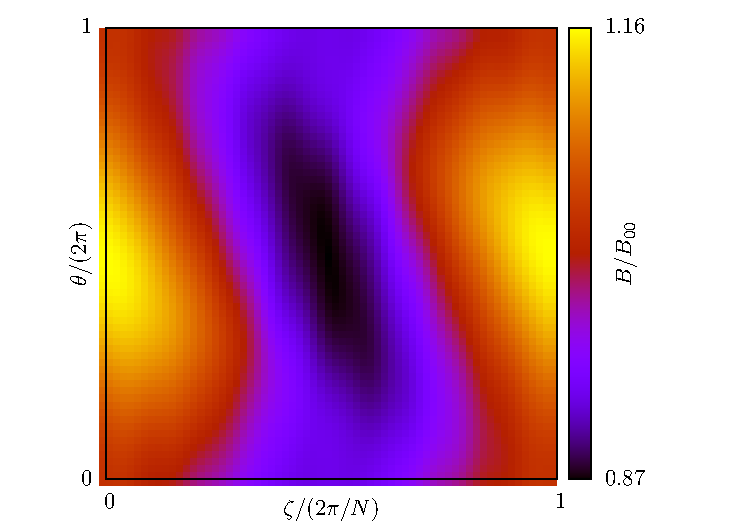
\includegraphics[angle=0,width=0.45\columnwidth]{figures/Bw7x.pdf}
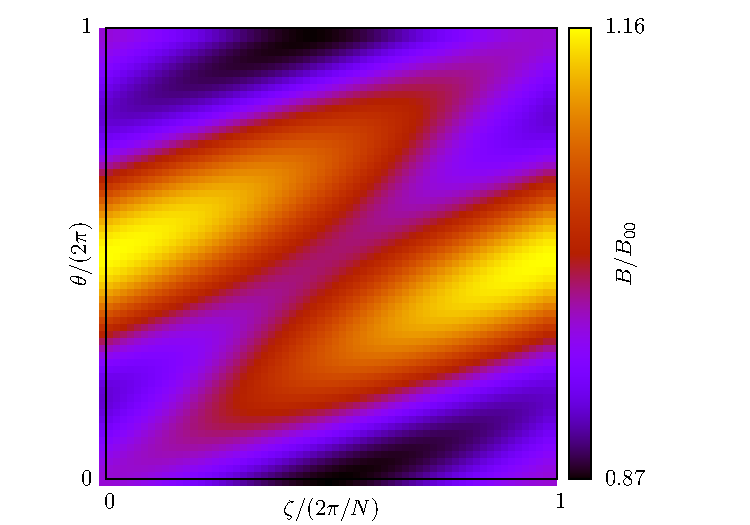
\includegraphics[angle=0,width=0.45\columnwidth]{figures/Blhd.pdf}
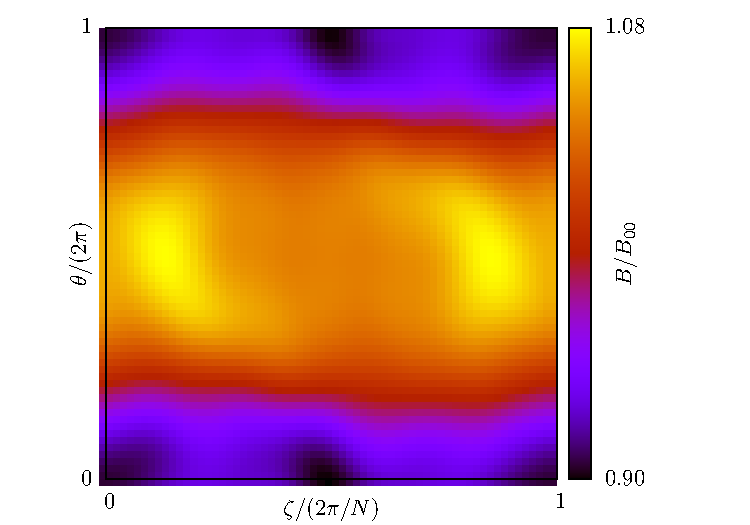
\includegraphics[angle=0,width=0.45\columnwidth]{figures/Bncsx.pdf}
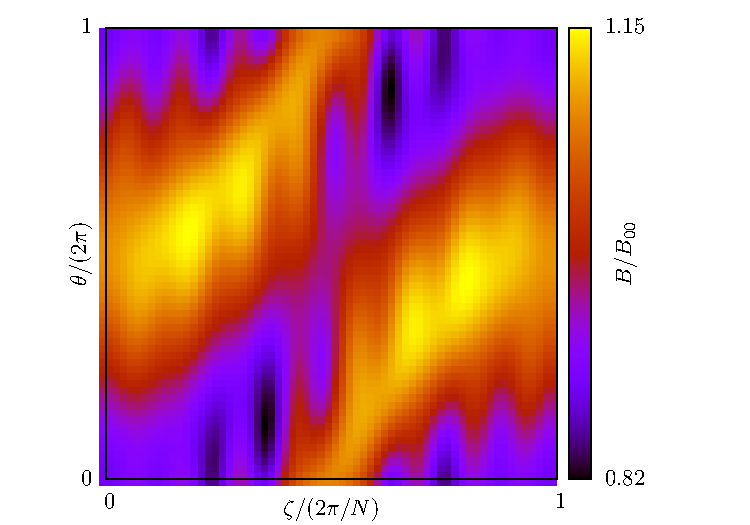
\includegraphics[angle=0,width=0.45\columnwidth]{figures/Btj2.pdf}
\caption{Magnetic field strength for surface $\psi/\psi_{LCFS}=0.5$ of the W7-X high-mirror configuration (top left), the LHD $R_{ax}=3.75\,$m configuration (top right), an NCSX equilibrium (bottom left) and the TJ-II standard configuration (bottom right).}
\label{FIG_MAP}
\end{figure}

\footnote{The input and output files of these simulations are provided in folder 'KNOSOS/TESTS/MONO', so that the user can reproduce them.} In this section, we will show that~\KNOSOS~can be used for creating a \DKES-like database of monoenergetic transport coefficients at low collisionalities. We will compare our calculations with~\DKES, both in results and computing time. Let us first discuss the rationale behind the monoenergetic approach, which is not specific to~\DKES, and the particular simplifications involved in~\DKES. More details can be found in the overview paper~\citep{beidler2011icnts}.

Predictive transport simulations solve the energy transport equation for every species:
\begin{equation}
\frac{3}{2}\frac{\partial n_bT_b}{\partial t}+ \frac{1}{r}\frac{\partial}{\partial r}(r Q_b)= \fsa{P_b}\,,
\end{equation}
where $P_b$ is the net energy input to species $b$ and the energy flux $Q_b$ contains a turbulent contribution, at least close to the edge, that is currently provided by simplified models~\citep{turkin2011predictive}. Calculating the time evolution of the energy, as in~\citep{sunnpedersen2015op11}, or finding the steady-sate solution as in~\citep{geiger2014w7x}, requires evaluating the neoclassical contribution to $Q_b$ a large number of times. The monoenergetic approach, together with some simplifications to the drift-kinetic equation, provides a way out of solving the drift-kinetic equation many times.

Strictly speaking, monoenergetic transport coefficients can always be calculated if the velocity $v$ is a parameter in the drift-kinetic equation that is being solved, as in the case of equation~(\ref{EQ_NDKE}): one can rewrite
\begin{equation}
Q_b = \int_0^\infty\mathrm{d} v D_{11,b}\frac{m_bv^2}{2} F_{M,b} \Upsilon_b\frac{\partial\psi}{\partial r}
\end{equation}
as a {\textit{convolution}} of monoenergetic transport coefficients
\begin{equation}
D_{11,b} = 2\left(\frac{\partial r}{\partial\psi}\right)^2\left\langle\int_{B^{-1}_{{\rm max}}}^{B^{-1}}\mathrm{d}\lambda\frac{v^3 B}{|v_\parallel |}\frac{g_b}{F_{M,b}\Upsilon_b}\mathbf{v}_{D,b}\cdot\nabla\psi\right\rangle \,,
\label{EQ_D11}
\end{equation}
where $g_b$ is the solution of equation~(\ref{EQ_NDKE}). Up to this point, the reduction in computation time associated to the monoenergetic approach stems from the fact that $v$ is a parameter in equation (\ref{EQ_NDKE}), which is then easier to solve than a drift-kinetic equation with energy diffusion in the collision operator.

Additionally, some fundamental simplifications are done by~\DKES: instead of $Q_b$, it calculates
\begin{equation}
\hat Q_b=\fsa{\mathbf{\hat Q_b}\cdot\nabla r} = \int_0^\infty\mathrm{d} v \hat D_{11,b}\frac{m_bv^2}{2} F_{M,b} \Upsilon_b\frac{\partial\psi}{\partial r}\,,\label{EQ_HATQ}
\end{equation}
with 
\begin{equation}
\hat D_{11,b} = 2\left(\frac{\partial r}{\partial\psi}\right)^2\left\langle\int_{B^{-1}_{{\rm max}}}^{B^{-1}}\mathrm{d}\lambda\frac{v^3 B}{|v_\parallel |}\frac{\hat g_b}{F_{M,b}\Upsilon_b}\mathbf{v}_{M,b}\cdot\nabla\psi\right\rangle \,.
\end{equation}
Here, $\hat g_b$ is the solution of a modified version of equation~(\ref{EQ_NDKE}), simplified as
\begin{equation}
\hat I_{v_E,\alpha}(\alpha,\lambda)\partial_\alpha \hat g_b +  I_{v_{M,\psi}}(\alpha,\lambda) {v_{d,b}} F_{M,b}\Upsilon_b
= \nu_{\lambda,b} \partial_\lambda\left[ I_\nu(\alpha,\lambda) \partial_\lambda \hat g_b\right]\,.
\label{EQ_DKES}
\end{equation}
With respect to equations (\ref{EQ_NDKE}) and (\ref{EQ_D11}), we have set 
\begin{eqnarray}
\mathbf{v}_E\cdot\nabla\psi&=&0\,,\nonumber\\
I_{v_{M,\alpha}}&=&0\,,\nonumber\\
I_{v_{E,\psi}}&=&0\,,\label{EQ_BINTDKES}
\end{eqnarray}
and replaced $I_{v_{E,\alpha}}$ with
\begin{eqnarray}
\hat I_{v_{E,\alpha}}&=&\Psi_t'\partial_\psi\varphi_0\int_{l_{b_1}}^{l_{b_2}}\frac{B^2}{\fsa{B^2}} \frac{\mathrm{d}l}{\sqrt{1-\lambda B}}\,.
\end{eqnarray}
In other words, the effect of the tangential electric field and the tangential magnetic drift is ignored, and an incompressible $\mathbf{E}\times\mathbf{B}$ tangential drift is used (this last simplification is specific of~\DKES~and is not used by other codes in~\citep{beidler2011icnts}). While it is well known~\citep{calvo2017sqrtnu} that these effects need to be kept in the drift-kinetic equation for an accurate computation of the radial fluxes, there is a range of situations in which $\hat Q_b\approx Q_b$ (this will be discussed in detail in \S\ref{SEC_TANGVM}) and this inaccuracy allows for a very large reduction of the computing time. The reason is that, for a given flux-surface, when normalized by the plateau value
\begin{eqnarray}
\hat D_{11}^*&\equiv& \frac{\hat D_{11,b}}{D_{11,b}^p}\,,\nonumber\\
D_{11,b}^p&=& \frac{\pi v_{d,b}^2 R_0}{4v\iota}\,,
\end{eqnarray}
the transport coefficients $\hat D_{11}^*$ only depend on two $v$-dependent dimensionless parameters, the collisionality 
\begin{equation}
\nu_{*}=\frac{R_0\nu_\lambda}{\iota v}\,,
\end{equation}
and the normalized radial electric field
\begin{equation}
v_{E*}=\frac{E_r}{v B_{0,0}}\,.
\end{equation}
Here, $R_0$ is the major radius, and the main Fourier mode of $B$ (see \S\ref{SEC_DELTA}) is $B_{0,0}\sim 1\,$T in all the simulations presented in this paper. Since there is no species dependence, in the rest of the section, we follow the common practice of dropping the species index when discussing monoenergetic calculations. A predictive transport simulation thus requires to precompute a so-called database of (\DKES-like) monoenergetic coefficients $\hat D_{11}^*( \nu_*,v_{E*}$). Once this is done, the calculation of $\hat Q_b$ for given $n_b$, $T_b$ and $E_r$ using equation~(\ref{EQ_HATQ}) requires a few bidimensional interpolations and an integral in $v$. The problem then lies in the computation of the database $\hat D_{11}^*( \nu_*,v_{E*})$ for every new magnetic configuration, which typically takes hours, due to the poor convergence of~\DKES~(and most neoclassical codes~\citep{beidler2011icnts}) at low collisionalities. We will show that the bounce-average technique greatly reduces the computing time by using in~\KNOSOS~equation (\ref{EQ_DKES}) and comparing the results with~\DKES. Calculations without the simplifications made by~\DKES~are left for \S\ref{SEC_TANGVM}.

In order to illustrate the performance of~\KNOSOS~in a variety of three-dimensional configurations, we choose four very different types of stellarators. Figure~\ref{FIG_MAP} shows the map of the magnetic field strength on the flux-surface  $\psi/\psi_{LCFS}=0.3$ of the high-mirror configuration of the helias W7-X (top left), the $R_{ax}=3.75\,$m configuration of the heliotron LHD (top right), an equilibrium of NCSX close to  quasiaxisymmetry (bottom left) and the standard configuration of the heliac TJ-II~(bottom right)\citep{ascasibar2019iaea}. 

\begin{figure}
\centering
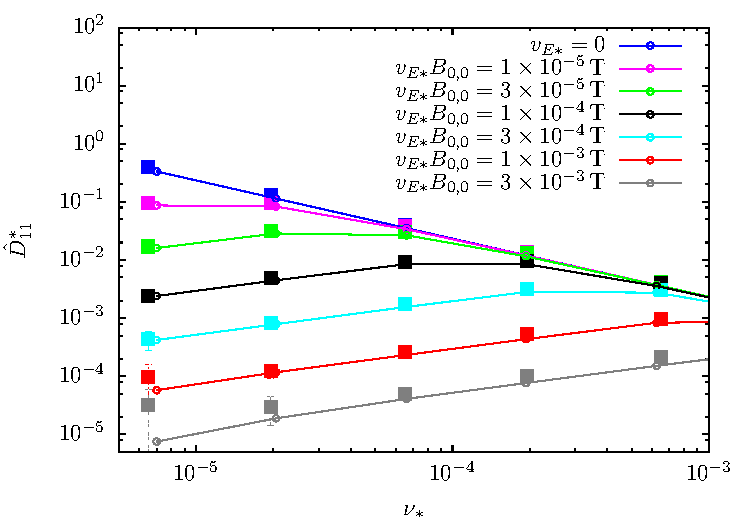
\includegraphics[angle=0,width=0.45\columnwidth]{figures/d11w7x.pdf}
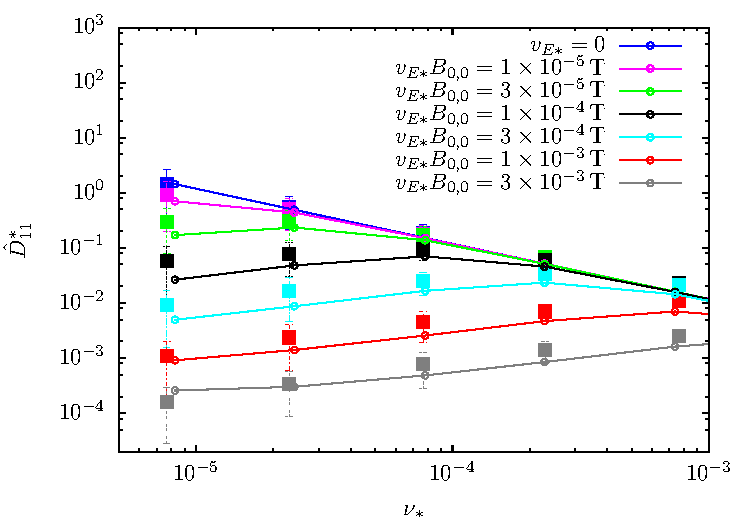
\includegraphics[angle=0,width=0.45\columnwidth]{figures/d11lhd.pdf}
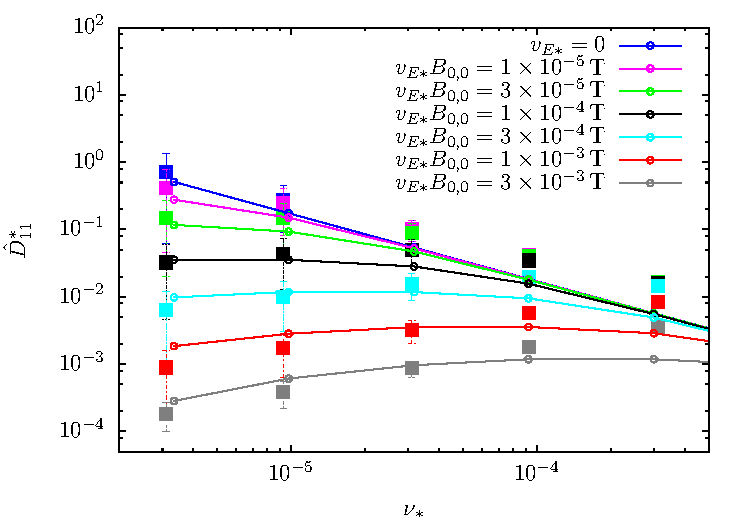
\includegraphics[angle=0,width=0.45\columnwidth]{figures/d11ncsx.pdf}
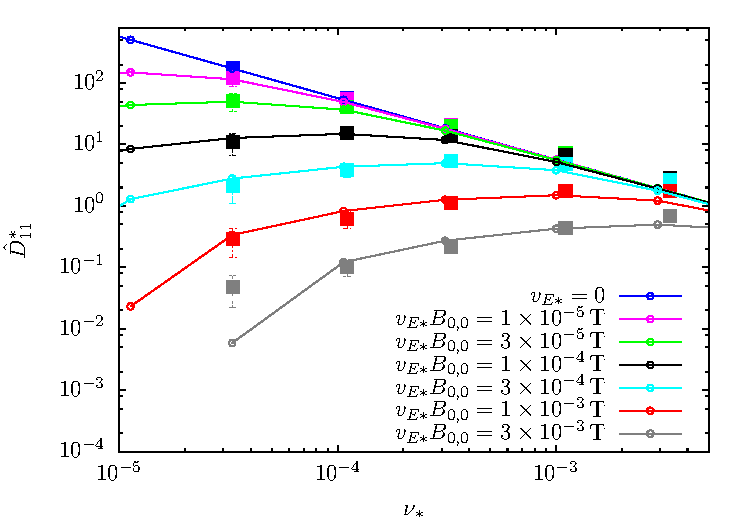
\includegraphics[angle=0,width=0.45\columnwidth]{figures/d11tj2.pdf}
\caption{Monoenergetic transport coefficients calculated with~\DKES~(full squares) and~\KNOSOS~(small open circles with lines) as a function of the collisionality at $\psi/\psi_{LCFS}=0.5$ surface of W7-X (top left), LHD (top right), NCSX (bottom left) and TJ-II (bottom right). The colour code is: $v_{E*}B_{0,0}=0$ (blue),  $1\times 10^{-5}\,$T (magenta),  $3\times 10^{-5}\,$T (green),  $1\times 10^{-4}\,$T (black),  $3\times 10^{-4}\,$T (cyan),  $1\times 10^{-3}\,$T (red),  and $3\times 10^{-3}\,$T (grey).}
\label{FIG_D11}
\end{figure}


Figure~\ref{FIG_D11} shows the first comparisons between~\KNOSOS~and~\DKES, in which the normalized monoenergetic transport coefficient $\hat D_{11}^*$ is calculated for several values of the collisionality and the normalized radial electric field.  Figure~\ref{FIG_D11} (top left) contains data for the W7-X high-mirror configuration, which we discuss in more detail. The expected $1/\nu$ dependence is observed at the highest collisionalities and, due only to the absence of tangential magnetic drift, for small values of $v_{E*}$. There is $\sqrt{\nu}$ characteristic behaviour elsewhere, with smaller levels of transport for larger $|E_r|$. The comparison between~\KNOSOS~and~\DKES~is satisfactory, with agreement within the error bars of the~\DKES~calculation, and only at the highest collisionalities, and for the largest values of $E_r$,  there are very small differences. The calculation for all the points of this case was made with ${\cal{N}}_\alpha=32$   and ${\cal{N}}_\lambda=64$, and it took $2.0$ seconds in a single standard CPU. Of this time, around $0.7$ seconds were used for setting the grid and performing the bounce-averages, and then it took less than $0.04$ seconds to calculate each point. This number may be reduced even further using smaller ${\cal{N}}_\lambda$ for the cases of largest collisionality and smallest radial electric field. In the $\sqrt{\nu}$ regime, transport is given by a small layer close to the boundary between passing and trapped particles. The size in $\lambda$ of this layer is proportional to $\sqrt{\nu_\lambda/E_r}$~\citep{calvo2017sqrtnu}, and this determines the required number of grid points ${\cal{N}}_\lambda$ in the low collisionality cases with radial electric field.
\begin{figure}
\centering
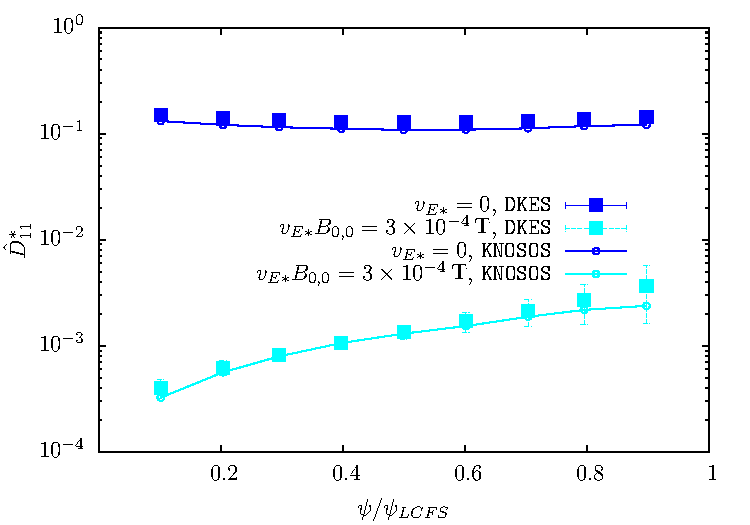
\includegraphics[angle=0,width=0.45\columnwidth]{figures/d11w7x_prof.pdf}
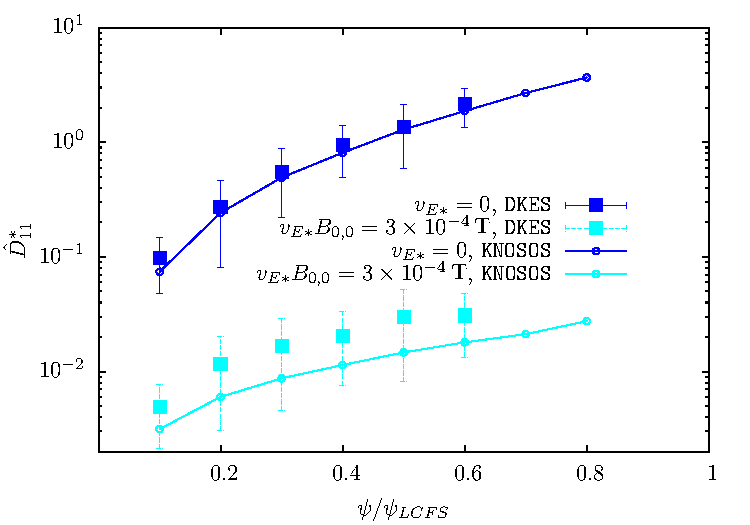
\includegraphics[angle=0,width=0.45\columnwidth]{figures/d11lhd_prof.pdf}
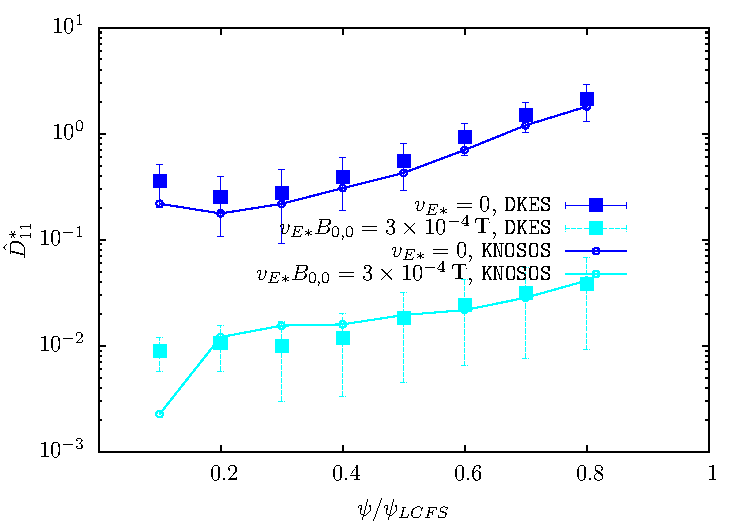
\includegraphics[angle=0,width=0.45\columnwidth]{figures/d11ncsx_prof.pdf}
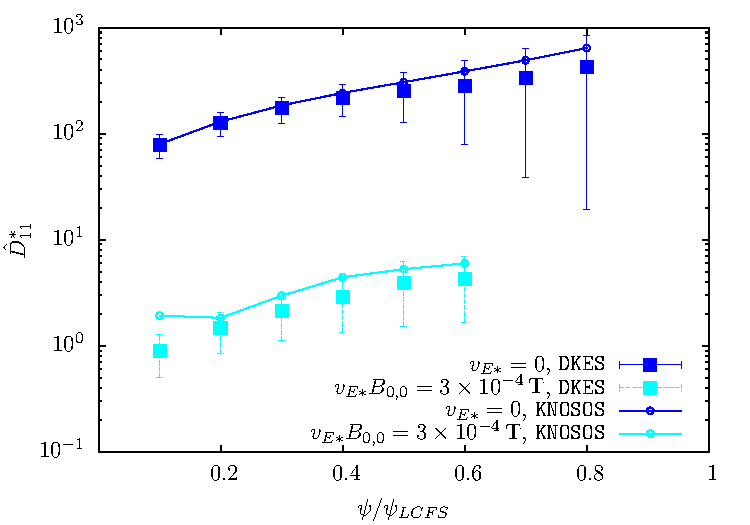
\includegraphics[angle=0,width=0.45\columnwidth]{figures/d11tj2_prof.pdf}
\caption{Radial profile of normalized monoenergetic transport coefficient calculated with~\DKES~(full squares) and~\KNOSOS~(small open circles with lines) for W7-X (top left), LHD (top right), NCSX (bottom left) and TJ-II (bottom right). Cyan corresponds to the $\sqrt{\nu}$ regime ($v_{E*}B_{0,0}=3\times 10^{-4}\,$T) and blue to the $1/\nu$ regime ($v_{E*}=0$).}
\label{FIG_D11PROF}
\end{figure}

Similar results can be seen for LHD in figure~\ref{FIG_D11} (top right). ${\cal{N}}_\alpha=32$  and ${\cal{N}}_\lambda=64$ grid points were used, and the total computation time was 2.1 seconds. For NCSX,  figure~\ref{FIG_D11} (bottom left), the agreement is good except for the higher collisionalities, where the $1/\nu$ regime should connect with a banana regime (see figure 15 of~\citep{beidler2011icnts}). This regime could be easily implemented in~\KNOSOS~following~\citep{landreman2012omni}. ${\cal{N}}_\alpha=32$  and ${\cal{N}}_\lambda=64$ grid points were used, and the total computation time was 1.0 seconds. Finally, figure~\ref{FIG_D11} (bottom right) contains the results for TJ-II, the hardest case due to its complicated magnetic geometry, see figure~\ref{FIG_MAP} (bottom right). ${\cal{N}}_\alpha=32$  and ${\cal{N}}_\lambda=128$ were used, and the simulation took 157 seconds.  Here, one can see more clearly that the cases deeper in the $\sqrt{\nu}$ regime are more difficult to converge, and indeed the points corresponding to $v_{E*}B_{0,0} \geq 10^{-3}\,$T and $\nu_*< 10^{-4}$ are barely converged. The rest of the simulations agree with~\DKES~and reach even lower collisionalities than those typically required for describing a TJ-II plasma, whose ion temperature never exceeds a few hundred eV.
 


Figure~\ref{FIG_D11PROF} contains, for each of the four configurations, radial profiles of the transport coefficient $\hat D^*_{11}$ for two cases, $v_{E*}=0$ and $v_{E*}B_{0,0}=3\times 10^{-4}\,$T, for a given collisionality.  They are meant to represent the level of transport in the $1/\nu$ regime ($\hat D^*_{11}$ is by definition proportional to $\epsilon_{eff}^{3/2}$, being $\epsilon_{eff}$ the effective ripple) and  the $\sqrt{\nu}$ regime, respectively. We choose $\nu_*=2\times 10^{-5}$  for W7-X (top left) and LHD (top right), $\nu_*=10^{-5}$ for NCSX (bottom left) and $\nu_*=3\times 10^{-5}$ for TJ-II (bottom right). It can be observed that the good agreement holds for all cases at all radial positions. The comparison of the different parts of figure~\ref{FIG_D11PROF} provides additional information that may be relevant when devising a stellarator optimization strategy: in general, configurations with lower $1/\nu$ transport show lower $\sqrt{\nu}$ transport as well. This is not surprising considering that both quantities are connected to the bounce-averaged radial component of the magnetic drift, which appears in the source of the drift-kinetic equation~(\ref{EQ_DKEFINAL}) in both regimes, and which is in turn proportional to the variation of the second adiabatic invariant on the flux-surface, $\partial_\alpha J$. Inasmuch as the optimization procedure actually reduces the size of $\partial_\alpha J$, both the $1/\nu$ and $\sqrt{\nu}$ (and superbanana-plateau) regimes will generally be optimized. Nevertheless, using directly the effective ripple as figure of merit of neoclassical transport does not automatically guarantee a reduction of $\partial_\alpha J$, and the $\sqrt{\nu}$ transport may remain unoptimized. Figure~\ref{FIG_D11PROF}  (top) may represent an example of this situation: while this W7-X configuration is designed to have low level of $1/\nu$ transport at an intermediate radial position (where the plasma volume is relatively large and neoclassical transport is expected to be at least comparable to anomalous transport), the $\sqrt{\nu}$ transport is smallest exactly at the magnetic axis. We will argue the relevance of optimizing transport regimes of collisionality lower than the $1/\nu$, which has now become possible with~\KNOSOS, in the next section.


%%%%%%%%%%%%%%%%%%%%%%%%%%%%%%%%%%%%%%%%%%%%%%%%%%%%%%%%%%%%%%%%%%%%%%%%%%%%%%%%%%%%%%%%%%%%%%%%%%%%%%%%%%%%%%%%%%%

\section{Effect of the tangential magnetic drift on the radial transport of energy}\label{SEC_TANGVM}

%%%%%%%%%%%%%%%%%%%%%%%%%%%%%%%%%%%%%%%%%%%%%%%%%%%%%%%%%%%%%%%%%%%%%%%%%%%%%%%%%%%%%%%%%%%%%%%%%%%%%%%%%%%%%%%%%%%

\footnote{The input and output files of these simulations are provided in folder 'KNOSOS/TESTS/AMB', so that the user can reproduce them.} In \S\ref{SEC_DKES}, we have shown solutions of equation~(\ref{EQ_DKES}), a simplified drift-kinetic equation that is not accurate when the tangential components of the magnetic drift and of the electric field play a role. In this section, we will demonstrate the importance of solving equation~(\ref{EQ_NDKE}) instead of equation~(\ref{EQ_DKES}), i.e., of computing $Q_b$ and not $\hat Q_b$, when calculating the radial energy flux in real plasmas. It must be noted that the solution of equation~(\ref{EQ_NDKE}) with~\KNOSOS~is not computationally more expensive than that of equation (\ref{EQ_DKES}): in the superbanana-plateau regime, that may arise in the presence of the tangential magnetic drift for certain values of $E_r$, transport is dominated by a resonant layer whose size decreases with $(\nu_\lambda/E_r)^{1/3}$, i.e., slower than the boundary layer that determines the $\sqrt{\nu}$ transport~\citep{calvo2017sqrtnu}. Calculating $Q_b$ instead of $\hat Q_b$ does not require a larger value of ${\cal{N}}_\lambda$ in general.

In this section, we focus on characterizing the effect of the tangential magnetic drift for the particular case of $\varphi_1=0$. We advance one of the salient results: this effect will be non-negligible even at not very low collisionalities. The reason is that the calculation of the energy flux for a given plasma, characterized by the kinetic profiles, requires the solution of the drift-kinetic equation for several values of the velocity, see equation~(\ref{EQ_CONV}), with the normalized particle energy $(v/v_{th,b})^2$ spanning several orders of magnitude. This means that, even if the thermal particles are in $1/\nu$ regime, there are particles with higher $v$ that are in lower collisionality regimes. 

Figure~\ref{FIG_QER1} contains simulations for the high-mirror configuration of W7-X at $\psi/\psi_{LCFS}=0.25$, which corresponds to $r/a=0.5$. We choose a pure hydrogen plasma, with $n_e=8.0\times 10^{19}\,$m$^{-3}$, $\partial_r n_e/n_e=-2.0\,$m$^{-1}$, $T_e = T_i = 4.0\,$keV, $\partial_r T_e/T_e =\partial_r T_i/T_i = -3.0\,$m$^{-1}$. These are values comparable to those measured in high-performance OP1.2 plasmas of W7-X~\citep{klinger2019op12} in the region of crossover between positive and negative radial electric field, corresponding to electron and ion root solutions of the ambipolarity equation~\citep{pablant2019ionroot}. In these plasmas, neoclassical transport calculated neglecting the tangential magnetic drift typically accounts for around half the total experimental transport. Figure~\ref{FIG_QER1} (top) contains a plot, in logarithmic scale, of the ion and electron radial energy flux as a function of the radial electric field. Empty and full blue boxes correspond to $\hat Q_i$ and $Q_i$ respectively, both calculated with~\KNOSOS. We immediately see that $\hat Q_i$ overestimates the radial energy flux at small values of the radial electric field, specially at $E_r = 0$ (strictly the only point of the figure where $\hat Q_i$ is proportional to $\varepsilon_{eff}^{3/2}$). The tangential drifts make the ion flux decrease, differently in the case of $\hat Q_i$ and $Q_i$, as we will discuss below. Finally, empty and full red boxes correspond to $\hat Q_e$ and $Q_e$ calculated with~\KNOSOS. In this plot, is difficult to notice any difference between the different electron calculations. Figure~\ref{FIG_QER1} (top) contains additional black lines that are the result of combining calculations with~\DKES~and~\KNOSOS. We will leave the discussion of these results for the end of the section.

Figure~\ref{FIG_QER1} (bottom) contains a blowup in linear scale of the most relevant range of the data in figure~\ref{FIG_QER1} (top). Here, the effect of the tangential magnetic drift on the energy flux can be observed more clearly: the size of the peak at small $|E_r|$ is reduced and displaced to positive (negative) values in the case of electrons (ions). The effect is larger for the ions due to their larger normalized Larmor radius $\rho_{i*}$, which makes them leave the $1/\nu$ regimes at relatively higher collisionalities. We have mentioned that these plasmas are close to the crossover between ion and electron root, and this figure can help us discuss some features of transport in both situations. In electron root, the radial electric field is expected to be positive and large, and the electrons are expected to give the largest contribution to energy transport. According to figure~\ref{FIG_QER1} (bottom), $Q_e$ provides a minor, although systematic, correction to $\hat Q_e$, below 10\% for this plasma profiles and configuration. The situation is different in ion root, typically characterized by a negative radial electric field that is small in size, and dominant ion transport. Here, including the tangential magnetic drift can lead to large corrections, above 50\% in some cases.

For the sake of completeness, figure~\ref{FIG_QER2} contains two more cases. In figure~\ref{FIG_QER2} (top) we repeat the calculation for a W7-X plasma of much higher collisionality, choosing $n_e=1.6\times 10^{20}\,$m$^{-3}$, $\partial_r n_e/n_e=-2.0\,$m$^{-1}$, $T_e = T_i = 2.5\,$keV, $\partial_r T_e/T_e =\partial_r T_i/T_i = -3.0\,$m$^{-1}$. We first note that the electrons are deep in the $1/\nu$ regime, since $\nu_{e*}=3.4\times 10^{-2}$ and $\rho_{e*}=1.4\times 10^{-5}$. Nevertheless, $Q_e(E_r)$ does not show the linear dependence expected when the $1/\nu$ dominates. This is an indication of what we advanced at the beginning of this section: even in plasmas nominally in the $1/\nu$ regime, the contribution of the $\sqrt{\nu}$ regime is not negligible, and should not be neglected in the optimization procedure. For the ions, even at these higher collisionalities and low temperatures, $\nu_{i*} = 1.6\times 10^{-2}$ is not much larger than $\rho_{i*} = 6.0\times 10^{-4}$ divided by the inverse aspect ratio. This means that, for ions slightly more energetic than the thermal ions, the tangential magnetic drift is relevant at small values of $|E_r|$~\citep{calvo2018jpp}. Figure~\ref{FIG_QER2} (top) shows indeed systematic differences between $\hat Q_i$ and $Q_i$. 

Finally, figure~\ref{FIG_QER2} (bottom) contains a calculation with the same kinetic profiles of figure~\ref{FIG_QER1} (top) for the inward-shifted configuration of LHD. It can be observed that the effects discussed in figure~\ref{FIG_QER2} (top) are even more pronounced, to the extent of changing qualitatively the $Q_b(E_r)$ dependence (and making it more similar to that reported in~\citep{matsuoka2015tangential}: while practically any increase of $|E_r|$ causes a reduction of $Q_i$ in W7-X, this is not the case for LHD. For finite ion-root values of $E_r$, $Q_i(E_r)$ has a peak whose height is determined by superbanana-plateau transport. 

In light of these results, two comments related to stellarator optimization can be made. First, the fact that the monoenergetic transport coefficients respond to small tangential $\mathbf{E}\times\mathbf{B}$ drifts differently in the inward-shifted LHD, with respect to other configurations, was already discussed in~\citep{beidler2011icnts}, and it can be observed more clearly when calculating the energy flux including the tangential magnetic drift. We also note that part of the neoclassical optimization of W7-X comes from its large aspect-ratio, which tends to make the tangential magnetic drift smaller, when compared with the $E\times B$ drift. It is then clear than a systematic study of the different low-collisionality regimes, and their different configuration dependence, should be addressed when devising an stellarator optimization strategy. Second, a comprehensive optimization strategy will involve, at least, solving energy transport consistently with ambipolarity and quasineutrality. Along this section, we have compared $Q$ and $\hat Q$ at fixed $E_r$, but a more systematic study applied to real discharges of W7-X, including the experimental validation of $E_r$ predictions, is ongoing~\citep{carralero2019irw}.

Let us finally discuss the black lines of figures~\ref{FIG_QER1} and~\ref{FIG_QER2}, which correspond to combining simulations of~\DKES~and~\KNOSOS. As we have argued at the beginning of this section, calculating the radial energy flux requires solving the drift-kinetic equation for velocities $(v/v_{th,b})^2$ spanning from $\sim 10^{-2}$ to $\sim 10^{2}$, typically. Similarly to what we discussed for $v\gg v_{th,b}$, this means that particles with $v\ll v_{th,b}$ could be in the plateau regime, and they would not be described by equation~(\ref{EQ_NDKE}). In order to quantify this effect, and to show that it is negligible for the high-performance plasmas of W7-X, we perform calculations of $Q_i(E_r)$ and $Q_e(E_r)$ combining~\KNOSOS~with~\DKES. This can be done by rewriting equation~(\ref{EQ_GAMMAQ}) as
\begin{equation}
Q_b = D_{11,b}^p\int_0^\infty\mathrm{d} v \left[ H(v_0-v) \hat D^*_{11}(v) + H(v-v_0) D^*_{11}(v) \right] \frac{m_bv^2}{2}  F_{M,b} \Upsilon_b\,,
\label{EQ_DKESpKNOSOS}
\end{equation}
where $H$ is the Heaviside function, $v_0$ is a cut-off velocity, $\hat D^*_{11}(v)$ comes from~\DKES~in this case and
\begin{equation}
D^*_{11}(v) = \frac{D_{11,b}}{D_{11,b}^p}
\end{equation}
from~\KNOSOS. The latter is calculated according to equation~(\ref{EQ_D11}) solving the drift-kinetic equation that is correct at low collisionalities with $\varphi_1$ set to zero. In other words, monoenergetic transport coefficients $\hat D^*_{11}$ coming from~\DKES~are used above certain collisionality when performing the velocity integral and monoenergetic transport coefficients $D^*_{11}$ coming from~\KNOSOS~are used below that collisionality. The cut-off velocity $v_0$ must correspond to particles in the $1/\nu$ regime, which is correctly described by the two codes. This guarantees that both codes are employed in the parameter region where they are accurate (and fast).

In figures~\ref{FIG_QER1} and \ref{FIG_QER2} (bottom), the black lines corresponding to using equation~(\ref{EQ_DKESpKNOSOS}) barely separate from the solution of equation~(\ref{EQ_NDKE}). This means that the contribution of the plateau regime to the energy flux is negligible. Only for ions in the presence of very negative values of the radial electric field, in the high-density W7-X calculation, starts the black line to separate from the blue signs. This is to be expected: due to the approximate (exact in the case of $\hat Q_i$) $|E_r|^{-3/2}$-dependence of the transport coefficients in the $\sqrt{\nu}$, the contribution of low collisionalities to transport is reduced for very large values of $|E_r|$, and therefore the contribution of the plateau becomes non-negligible.

\begin{figure}
\centering
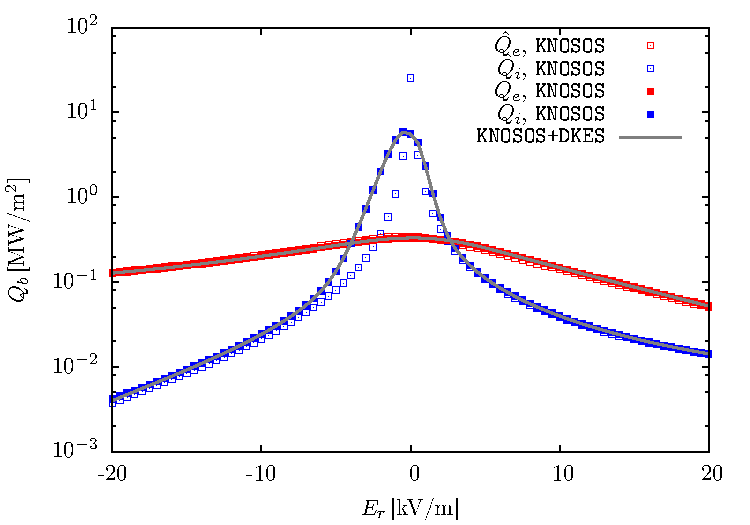
\includegraphics[angle=0,width=0.6\columnwidth]{figures/QEr.pdf}
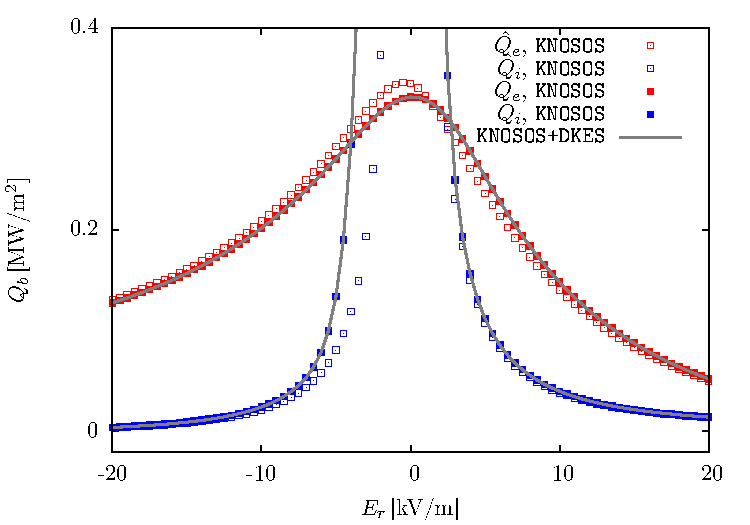
\includegraphics[angle=0,width=0.6\columnwidth]{figures/QEr_nolog.pdf}
\caption{Radial energy flux as a function of the radial electric field for a W7-X high-performance plasma: logarithmic (top) and linear (bottom) scale.}
\label{FIG_QER1}
\end{figure}

\begin{figure}
\centering
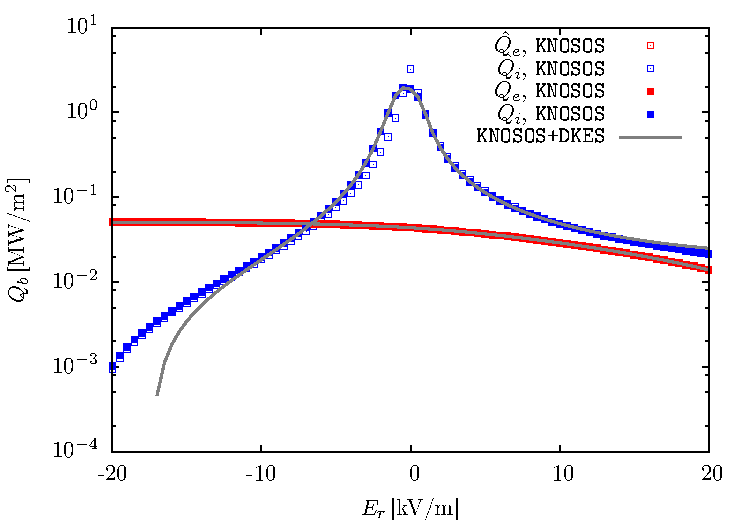
\includegraphics[angle=0,width=0.6\columnwidth]{figures/QEr_highn.pdf}
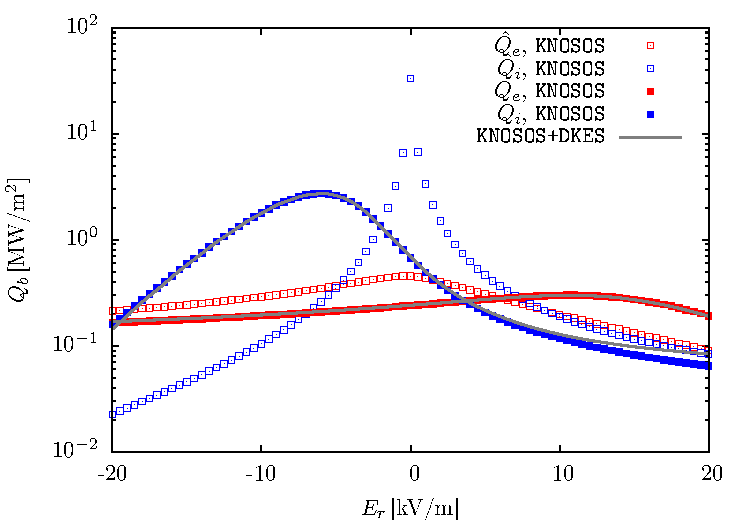
\includegraphics[angle=0,width=0.6\columnwidth]{figures/QEr_lhd.pdf}
\caption{Radial energy flux as a function of the radial electric field for a W7-X high density plasma (top) and an LHD plasma (bottom).}
\label{FIG_QER2}
\end{figure}

%%%%%%%%%%%%%%%%%%%%%%%%%%%%%%%%%%%%%%%%%%%%%%%%%%%%%%%%%%%%%%%%%%%%%%%%%%%%%%%%%%%%%%%%%%%%%%%%%%%%%%%%%%%%%%%%%%%

\section{Tangential electric field}\label{SEC_EUTERPE}

%%%%%%%%%%%%%%%%%%%%%%%%%%%%%%%%%%%%%%%%%%%%%%%%%%%%%%%%%%%%%%%%%%%%%%%%%%%%%%%%%%%%%%%%%%%%%%%%%%%%%%%%%%%%%%%%%%%

\begin{figure}
\begin{center}
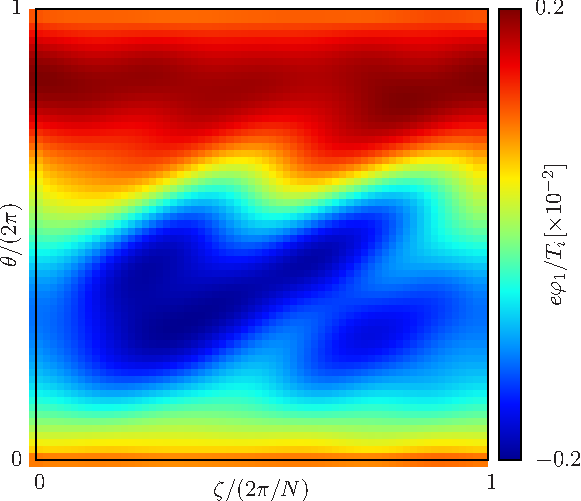
\includegraphics[width=0.3\columnwidth,angle=0]{figures/euterpeAIII02}
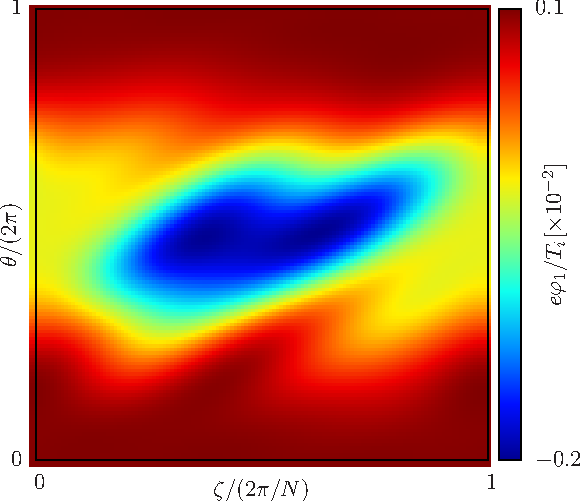
\includegraphics[width=0.3\columnwidth,angle=0]{figures/knososeutAIII02}
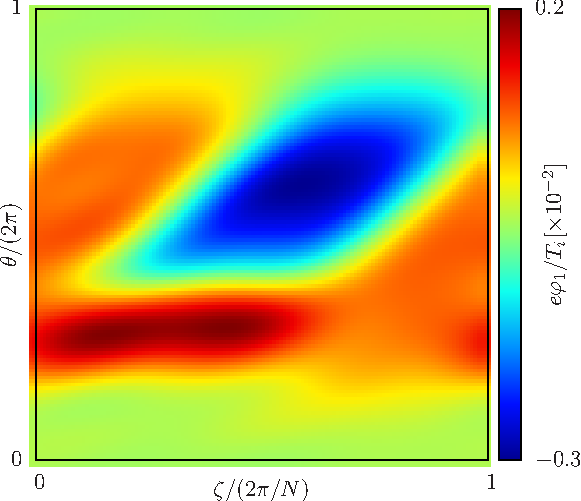
\includegraphics[width=0.3\columnwidth,angle=0]{figures/knososAIII02}

\

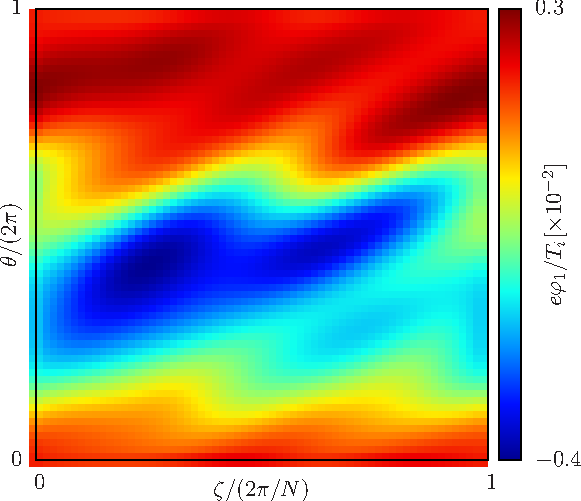
\includegraphics[width=0.3\columnwidth,angle=0]{figures/euterpeAIII04}
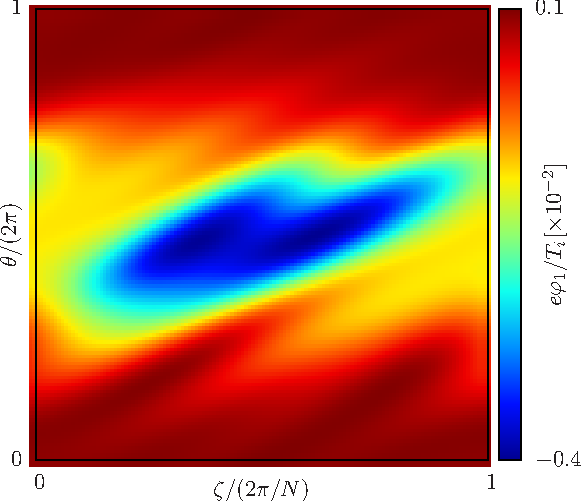
\includegraphics[width=0.3\columnwidth,angle=0]{figures/knososeutAIII04}
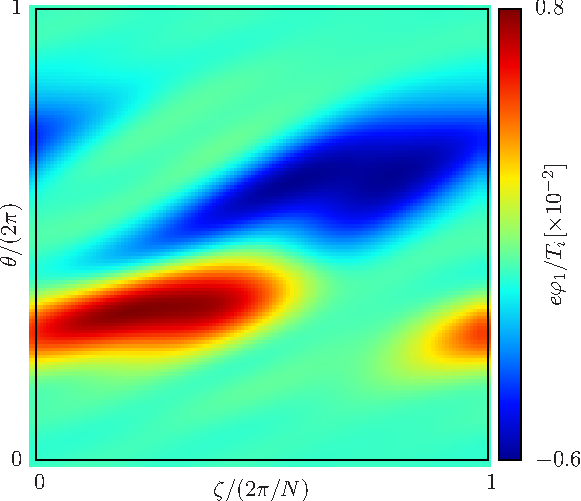
\includegraphics[width=0.3\columnwidth,angle=0]{figures/knososAIII04}

\

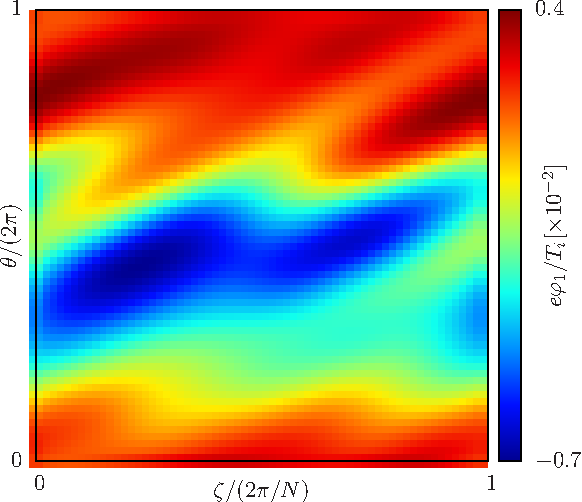
\includegraphics[width=0.3\columnwidth,angle=0]{figures/euterpeAIII06}
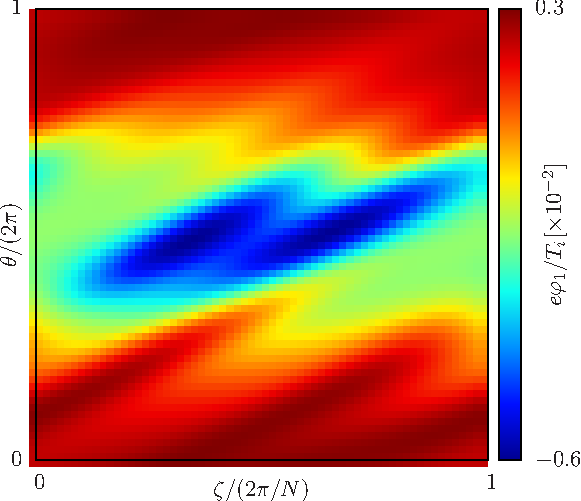
\includegraphics[width=0.3\columnwidth,angle=0]{figures/knososeutAIII06}
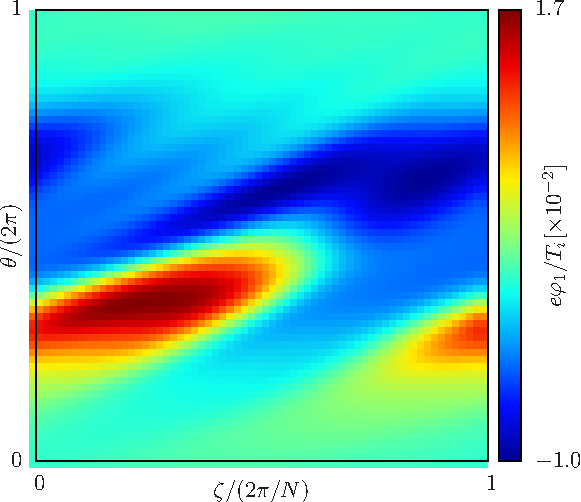
\includegraphics[width=0.3\columnwidth,angle=0]{figures/knososAIII06}

\

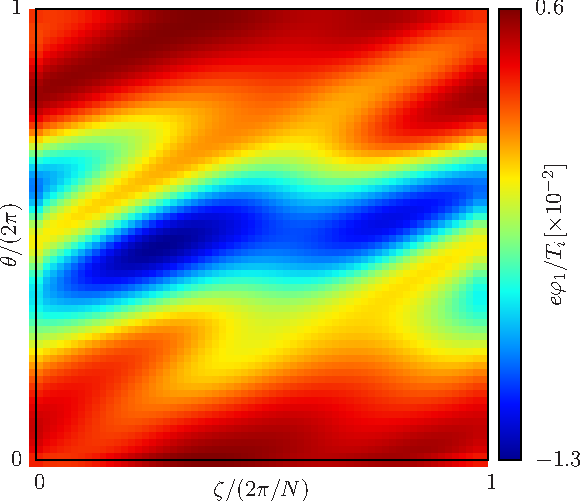
\includegraphics[width=0.3\columnwidth,angle=0]{figures/euterpeAIII08}
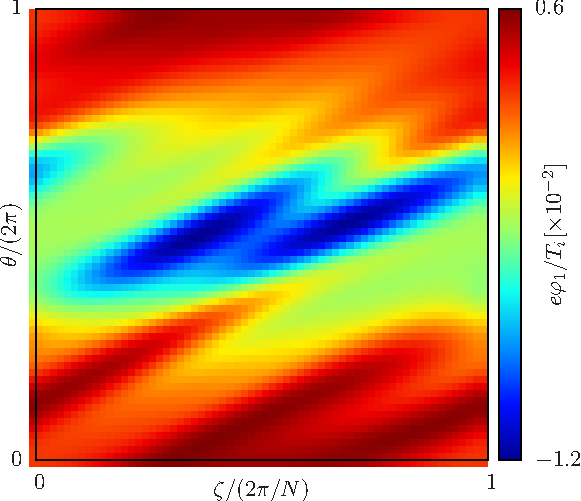
\includegraphics[width=0.3\columnwidth,angle=0]{figures/knososeutAIII08}
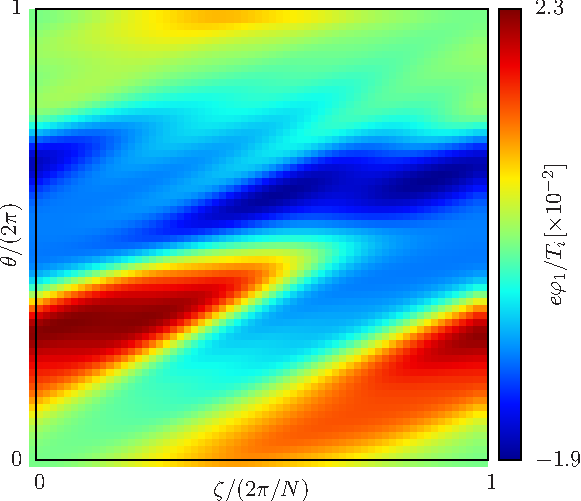
\includegraphics[width=0.3\columnwidth,angle=0]{figures/knososAIII08}
\end{center}
\caption{Electrostatic potential variation on the flux-surface calculated fort the LHD plasma with \texttt{EUTERPE} (left) and \texttt{KNOSOS} neglecting (center) and including (right) the tangential magnetic drift. The four rows correspond to radial positions $r/a\,=\,$0.2, 0.4, 0.6 and 0.8.}
\label{FIG_PHI1LHD}
\end{figure}

\begin{figure}
\begin{center}
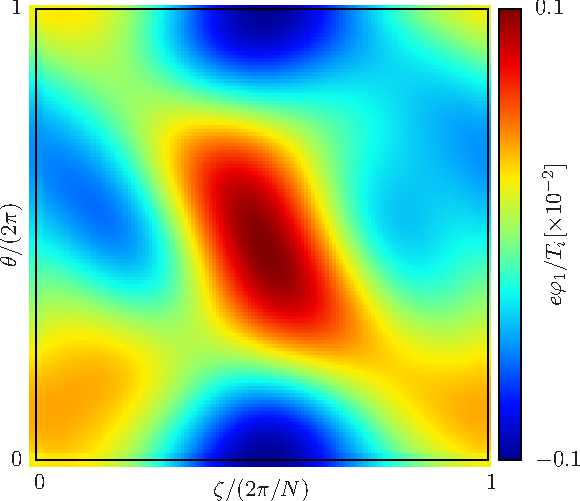
\includegraphics[width=0.3\columnwidth,angle=0]{figures/euterpeIV02}
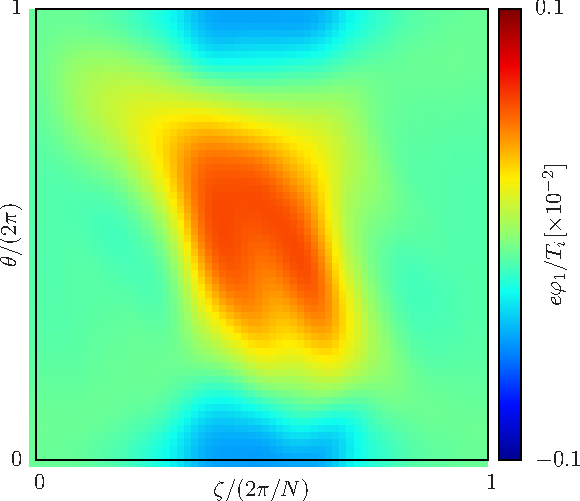
\includegraphics[width=0.3\columnwidth,angle=0]{figures/knososeutIV02}
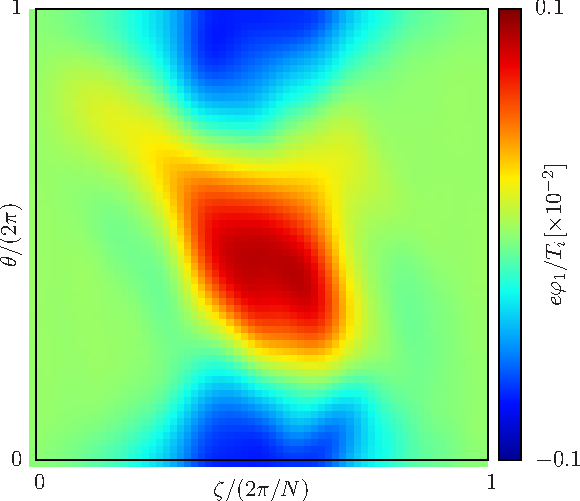
\includegraphics[width=0.3\columnwidth,angle=0]{figures/knososIV02}

\

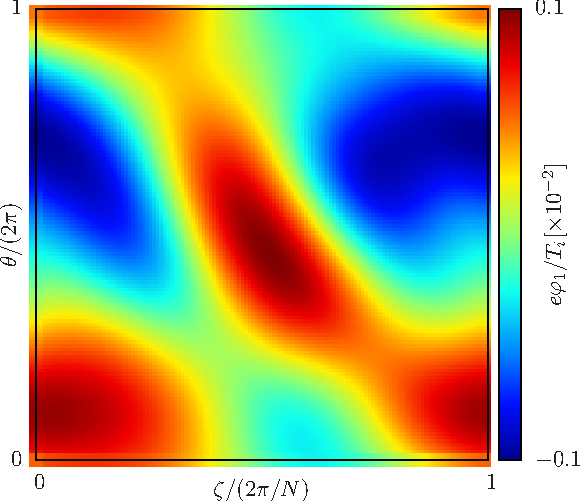
\includegraphics[width=0.3\columnwidth,angle=0]{figures/euterpeIV04}
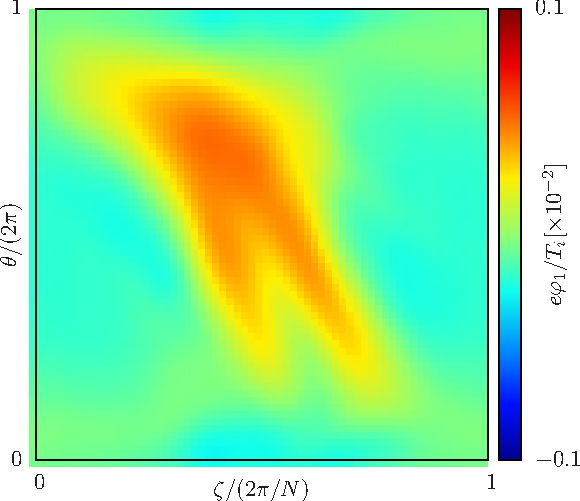
\includegraphics[width=0.3\columnwidth,angle=0]{figures/knososeutIV04}
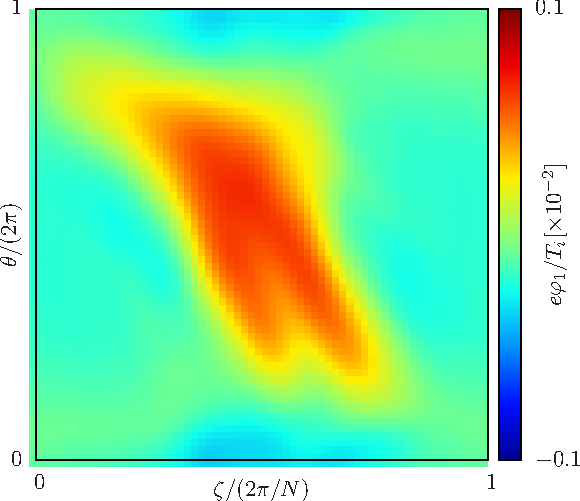
\includegraphics[width=0.3\columnwidth,angle=0]{figures/knososIV04}

\

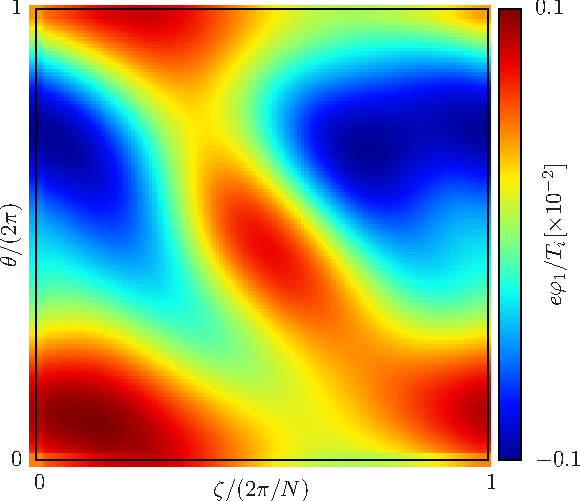
\includegraphics[width=0.3\columnwidth,angle=0]{figures/euterpeIV06}
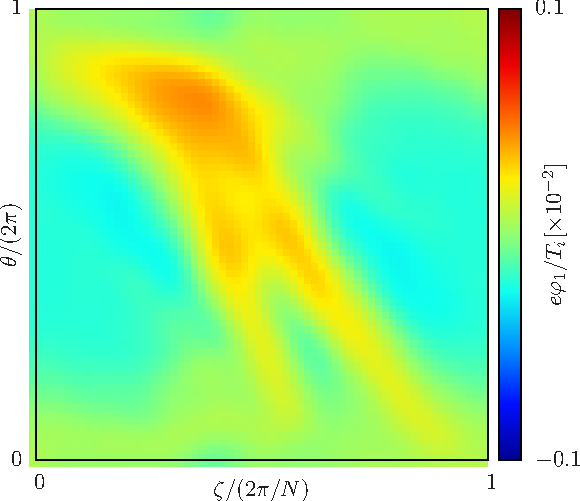
\includegraphics[width=0.3\columnwidth,angle=0]{figures/knososeutIV06}
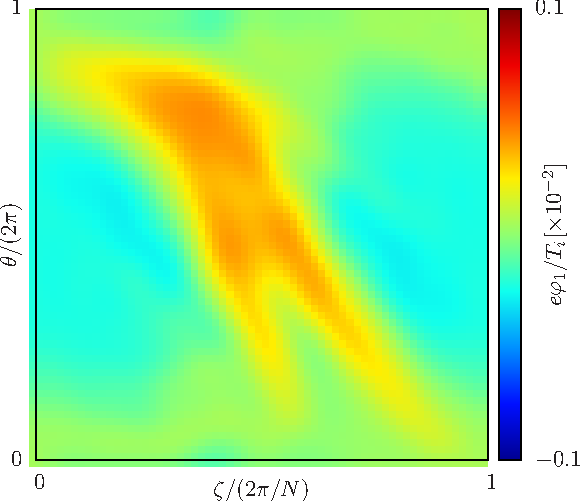
\includegraphics[width=0.3\columnwidth,angle=0]{figures/knososIV06}

\

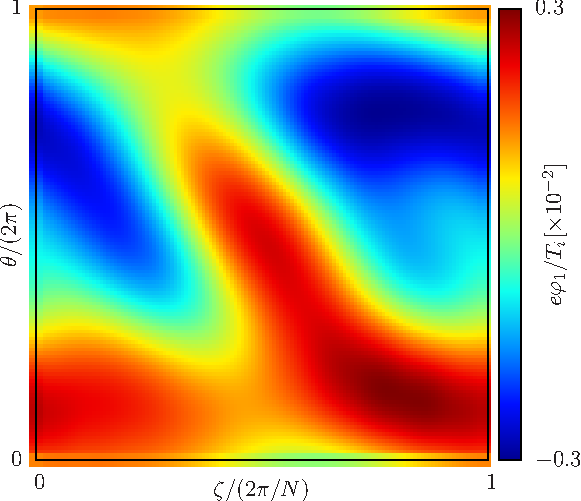
\includegraphics[width=0.3\columnwidth,angle=0]{figures/euterpeIV08}
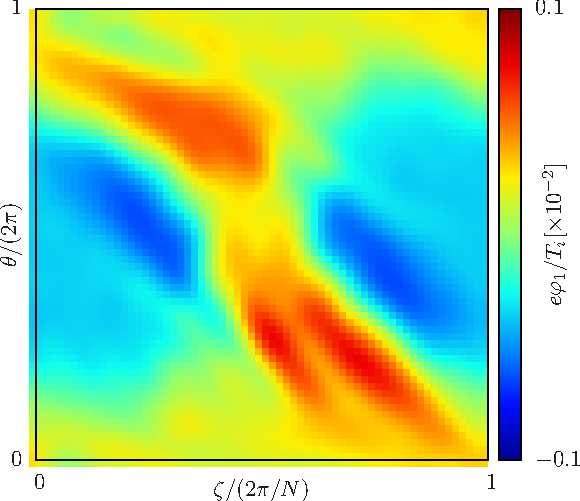
\includegraphics[width=0.3\columnwidth,angle=0]{figures/knososeutIV08}
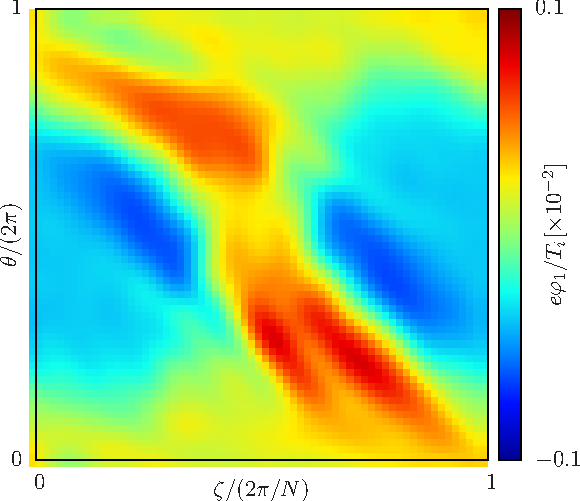
\includegraphics[width=0.3\columnwidth,angle=0]{figures/knososIV08}
\end{center}
\caption{Electrostatic potential variation on the flux-surface calculated fort the W7X plasma with \texttt{EUTERPE} (left) and \texttt{KNOSOS} neglecting (center) and including (right) the tangential magnetic drift. The four rows correspond to radial positions $r/a\,=\,$0.2, 0.4, 0.6 and 0.8.}
\label{FIG_PHI1W7X}
\end{figure}

\footnote{The input and output files of these simulations are provided in folder 'KNOSOS/TESTS/QN', so that the user can reproduce them.} Neoclassical physics gives rise to $\varphi_1$, and the associated tangential electric field produces radial drifts in all species. This is the reason why we need to solve consistently the drift-kinetic equations of the bulk species and quasineutrality~\citep{calvo2017sqrtnu}, but the effect is more relevant for impurities, due to their larger charge number, changing even qualitatively transport~(e.g. making it depend on the radial electric field in the so-called mixed collisionality regime~\citep{calvo2018nf,buller2018jpp}).  With impurity transport in mind, simulations of $\varphi_1$ for the stellarators W7-X, LHD and TJ-II have been performed in the last years with three codes,~\EUTERPE,~{\ttfamily SFINCS} and recently {\ttfamily FORTEC-3D}~\citep{regana2013euterpe,regana2017phi1,regana2018phi1,mollen2018phi1,fujita2019phi1}. Nevertheless, the number of simulations remains small because they are computationally very demanding, specially at low collisionalities. A more comprehensive study, including dependence on the configuration, collisionality, and bulk plasma profiles thus remains to be done.  In this section, we will show that~\KNOSOS~can reproduce the results of~\EUTERPE~(with adiabatic electrons and no tangential magnetic drift) and, by accounting for the effect of the tangential magnetic drift, describe stellarator regimes only simulated before for simplified geometries~\citep{calvo2018jpp,velasco2018phi1}. Since it can do so while keeping the computing time low, this opens the door to a number of new impurity transport studies. 

We start by reproducing the results of~\citep{regana2017phi1}, specifically of two low-collisionality plasmas of LHD and W7-X.  These are expected to be the plasma conditions of largest $e\varphi_1/T_i$ so that, even in optimized magnetic configurations, the effect on the radial transport of impurities may be large. It will be confirmed (as advanced in a previous work~\citep{velasco2018phi1} in a simplified calculation) that the inclusion of the tangential magnetic field leads to qualitative changes in $\varphi_1$, making it larger. Figure~\ref{FIG_PHI1LHD} shows the variation of the electrostatic potential on several flux-surfaces of the inward-shifted configuration of LHD for a low-collisionality plasma (described in~\citep{regana2017phi1}, termed AIII, and characterized by a small negative $E_r$). Each row corresponds to a different flux-surface, and each column to a different calculation method. Let us start by comparing the left column, calculated with~\EUTERPE, with the center column, calculated with~\KNOSOS~using equation (\ref{EQ_DKES}). The two methods should give the same results, and it can be observed that, although there are some differences, reasonable agreement between the two codes is obtained. It should be emphasized that differences in calculated values of $\varphi_1$ similar but smaller to those reported here, have been shown to produce negligible differences in impurity transport~\citep{velasco2018phi1}. If we now focus on the right column, we observe, as discussed in detail in~\citep{velasco2018phi1}, that the inclusion of the tangential produces relevant differences (in particular, more important than those between the left and center columns): the amplitude becomes larger, and the phase changes, with the angular dependence of $\varphi_1$ turning from being stellarator-symmetric (as expected for ions in the $\sqrt{\nu}$ regime), to not having definite symmetry (as corresponds to the superbanana-plateau regime~\citep{calvo2018jpp}).

Figure~\ref{FIG_PHI1W7X} contains a similar calculation performed for a low-collisionality plasma of W7-X (described in~\citep{regana2017phi1}, termed IV, and characterized by a larger negative $E_r$). Again, each row corresponds to a different flux-surface, and each column to a different calculation method. The comparison between~\EUTERPE~and~\KNOSOS~solving the same equation (left and center) is good close to the core, but it becomes slightly worse closer to the edge, where~\KNOSOS~underestimates the amplitude of $\varphi_1$. When the tangential magnetic drift is included (right), the results change very slightly in the core and do not change elsewhere. This feature is likely caused by the large radial electric field, which leaves the ions in the $\sqrt{\nu}$ regime (instead of the superbanana-plateau).

The computing time for each of these \KNOSOS~simulations is of the order of a minute in a single processor. We note that including kinetic electrons (which may be necessary for high electron temperature) would roughly double the computing time. This is to be compared with the $(m_i/m_i)^{1/2} \approx 43$ factor in Monte Carlo codes such as~\EUTERPE~and {\ttfamily FORTEC-3D}.

Let us finally mention that the experimental validation of $\varphi_1$ predictions has drawn much attention in the last years: experimental measurements of $\varphi_1$ were first obtained at the edge of the TJ-II stellarator~\cite{pedrosa2015phi1}, and very recently in its core region~\citep{estrada2019phi1}. The validation of~\KNOSOS~predictions, including finer scans in the magnetic configuration, is left for a forthcoming work.

\chapter{Concluding remarks}\label{CHAP_CONC}

%%%%%%%%%%%%%%%%%%%%%%%%%%%%%%%%%%%%%%%%%%%%%%%%%%%%%%%%%%%%%%%%%%%%%%%%%%%%%%%%%%%%%%%%%%%%%%%%%%%%%%%%%%%%%%%%%%%

\footnote{This chapter corresponds to section 5 of~\citep{velasco2019knosos}.}
{\ttfamily KNOSOS} is a freely-available open-source code that provides a fast computation of neoclassical transport at low collisionality in three-dimensional magnetic confinement devices, thanks to a rigorous application of the orbit-averaging technique to the drift-kinetic equation and an efficient solution of the quasineutrality equation. We have shown that, when solving equivalent equations, {\ttfamily KNOSOS} reproduces the calculations of~\DKES~and {\ttfamily EUTERPE} in simulations that can be orders of magnitude faster. This makes it a tool that can be used for a variety of physics problems, that we summarize next.

As a first obvious application, it can provide a fast calculation of the level of transport of a magnetic configuration for low-collisionality transport regimes not usually considered in stellarator optimization, such as the $\sqrt{\nu}$ and superbanana-plateau regimes. Optimization programmes are slowly starting to provide more a accurate characterization of transport by performing predictive simulations with prescribed sources and turbulent transport models. {\ttfamily KNOSOS} can also contribute to overcome two of the main limitations of this approach: the large computing time needed to create a database of mononoenergetic neoclassical transport coefficients and/or the lack of accuracy involved in the monoenergetic approach itself.
 
But a fast neoclassical code can have uses beyond stellarator optimization. For instance, the transport of impurities caused by their interaction with the bulk ions (via $\varphi_1$ or through inter-species collisions) has drawn much attention in the last years; however, a systematic study of its dependence on the magnetic configuration, colllisionality, and bulk plasma profiles remains to be done, due to the large computing resources needed for the combined solution of the quasineutrality and drift-kinetic equations of the bulk species. This will be addressed in forthcoming papers, in combination with analytical formulas for the radial flux of impurities in a variety of neoclassical regimes~\citep{calvo2018nf,calvo2019anis}.

Finally even in situations in which turbulence is dominant, a fast neoclassical code may be required. Its output (the radial electric field, the tangential electric field or the complete distribution function of the bulk species) can be read by gyrokinetic codes when studying the effect of neoclassical transport on turbulence. This effect is expected to be largest in those low-collisionality regimes in which the specificities of {\ttfamily KNOSOS} (very small computing time and inclusion of the tangential magnetic drift) are most relevant.


% Appendices
\appendix
\chapter{High collisionalities}\label{CHAP_HIGHCOL}

In this appendix we describe how the code solves transport at higher collisionalities (for which the bounce-average technique cannot be applied). For bulk species, we will recover the results of \DKES~(i.e., without momentum conservation), while for trace impurities we will obtain those of~\citep{calvo2018nf}.

%%%%%%%%%%%%%%%%%%%%%%%%%%%%%%%%%%%%%%%%%%%%%%%%%%%%%%%%%%%%%%%%%%%%%%%%%%%%%%%%%%%%

\section{Bulk species in the Pfisrch-Schl\"uter regime}

We repeat here the derivation of the appendix of~\citep{igitkhanov2006impurity}.  We want to calculate $h$, the deviation of the distribution function from the Maxwellian, and we assume $\varphi_1=0$. The equation that we want to solve is
\begin{equation}
\left(vp\frac{\bB}{B}+\frac{\bE\times\bB}{B^2}\right)\cdot\bnabla h + \bv_M\cdot\bnabla\psi \Upsilon F_M = \frac{\nu}{2}\frac{\partial}{\partial p}\left((1-p^2)\frac{\partial h}{\partial p}\right)\,.\label{EQ_DKEPS}
\end{equation}
where we have used a simplified collision operator that is not correct at these collisionalities. The variables in velocity space are the particle speed $v$ and the pitch-angle $p=v_\parallel/v$. Finally, we note that, for very high collisionalities, we have to keep the $\bE\times\bB$ drift. 

Using the expressions derived in \S\ref{SEC_USEFUL} for right-handed Boozzer coordinates, equation~(\ref{EQ_DKEPS})  becomes
\begin{eqnarray}
 \left[vp\frac{B}{B_\zeta+\iota B_\theta}\left(\iota\frac{\partial}{\partial \theta}+\frac{\partial}{\partial \zeta}\right)+ \frac{1}{|B_\zeta+\iota B_\theta|}\frac{\partial \varphi}{\partial\psi}\left(B_\zeta\frac{\partial}{\partial \theta}-B_\theta\frac{\partial}{\partial \zeta}\right)\right]  h +\nonumber\\ +v_d\frac{1+p^2}{2}\frac{1}{B|B_\zeta+\iota B_\theta|}\left(B_\theta\frac{\partial B}{\partial \zeta}-B_\zeta\frac{\partial B}{\partial \theta}\right) \Upsilon F_M = \frac{\nu}{2}\frac{\partial}{\partial p}\left((1-p^2)\frac{\partial h}{\partial p}\right)\,.
\end{eqnarray}
We now expand $h$ (and $B$) in Fourier components
\begin{equation}
h(\theta,\zeta,p) = \Upsilon F_M \sum_{m,n} h_{mn}(p)\exp{[i(m\theta+nN_p\zeta)]}\,,
\end{equation}
and $h_{mn}(p)$ in Legendre polynomia:
\begin{eqnarray}
h_{mn}(p) = \sum_l h_{mnl} P_l(p) = h_{mn0} + p h_{mn1} + \frac{1}{2}(3p^2-1) h_{mn2}\,.
\end{eqnarray}
We keep only the two first polynomia since it is easy to show that
\begin{eqnarray}
\int_{-1}^{+1}\mathrm{d}p (1+p^2) P_2(p) = 0.1 \int_{-1}^{+1}\mathrm{d}p (1+p^2) P_0(p)\,.
\end{eqnarray}
and, at large $\nu$, $h_{mn2}\ll h_{mn0}$. We now invoke the large aspect-ratio approximation and consider variations of the magnetic field strenght to be small compared to its average. In this limit
\begin{eqnarray}
\frac{B}{B_\zeta+\iota B_\theta} &\approx& \frac{\Psi_t'}{R}\,,\nonumber\\
\frac{1}{B} &\approx& \frac{1}{\overline{B}}\,,
\end{eqnarray}
where $R$ is the major radius of the device and $\overline{B}$ some average of the magnetic field strength\footnote{We take $\overline{B}\equiv B_{00}$.}. The drift-kinetic equation becomes, for each Fourier component
\begin{eqnarray}
i\left[vp\frac{\Psi_t'}{R}(\iota m  + nN_p)+\frac{1}{|B_\zeta+\iota B_\theta|}\frac{\partial \varphi}{\partial\psi}(m B_\zeta-nN_p B_\theta)\right] \left(h_{mn0} + p h_{mn1}+ \frac{1}{2}(3p^2-1) h_{mn2}\right) -\nonumber\\ +iv_d\frac{1+p^2}{2} \frac{1}{\overline{B}|B_\zeta+\iota B_\theta|} (n N_p B_\theta - m B_\zeta) B_{mn}  = \frac{\nu}{2} \left( -2 p h_{mn1} - 3(3p^2-1) h_{mn2}\right)\,.
\end{eqnarray}
and we have to solve a system of three equations
\begin{eqnarray}
i\omega_{mn}h_{mn0} + \left(-\frac{3}{2}\nu -i\frac{1}{2}\omega_{mn}\right)h_{mn2} = iv_{d,mn}\,,\nonumber\\
iu_{mn}h_{mn0} + (i\omega_{mn}+\nu) h_{mn1} = 0 \,,\nonumber\\
iu_{mn}h_{mn1}+\left(\frac{9}{2}\nu+i\frac{3}{2}\omega_{mn}\right)h_{mn2} = iv_{d,mn}\,,
\end{eqnarray}
where
\begin{eqnarray}
u_{mn} &=& v\frac{\Psi_t'}{R}(\iota m  + nN_p)\,,\nonumber\\
\omega_{mn} &=& \frac{\partial \varphi}{\partial\psi}(m B_\zeta-nN_p B_\theta)\,,\nonumber\\
v_{d,mn} & = &\frac{v_d}{2} \frac{1}{\overline{B}|B_\zeta+\iota B_\theta|} (m B_\zeta-n N_p B_\theta) B_{mn}  \,,
\end{eqnarray}
These equations can be combined into two:
\begin{eqnarray}
iu_{mn}h_{mn1} +i3\omega_{mn}h_{mn0} &=& i4v_{d,mn}\,,\nonumber\\
iu_{mn}h_{mn0} + (i\omega_{mn}+\nu) h_{mn1} &=& 0 \,,
\end{eqnarray}
and we can solve for $h_{mn0}$, the only one that contributes the the radial flux:
\begin{eqnarray}
h_{mn0} =i\frac{4v_{d,mn}u_{mn}^2\nu}{(u_{mn}^2-3\omega_{mn}^2)^2+(3\nu\omega_{mn})^2}\approx i\frac{4v_{d,mn}\nu}{u_{mn}^2\left[1+\left(\frac{3\nu\omega_{mn}}{u_{mn}^2}\right)^2\right]}\,,
\end{eqnarray}
where we have only kept the stellarator-asymmetric part and we have used that $u_{mn}^2\gg 3\omega_{mn}^2$. We can now calculate the neoclassical transport coefficient $D_{11}$ (note that we drop the species index):
\begin{equation}
D_{11}= -\frac{1}{2}\left(\frac{\partial r}{\partial\psi}\right)^2\fsa{\int_{-1}^{+1}\mathrm{d}p \frac{h}{\Upsilon F_M} \bv_M\cdot\bnabla\psi}\,,
\end{equation}
where the brackets denote flux-surface-average. Thanks to the large aspect-ratio approximation, we can take the Jacobian to be approximately constant and obtain 
\begin{eqnarray}
D_{11} \approx -\frac{1}{2}\left(\frac{\partial r}{\partial\psi}\right)^2\frac{1}{4\pi^2}\int_0^{2\pi}\mathrm{d}\theta\int_0^{2\pi}\mathrm{d}\zeta\int_{-1}^{+1}\mathrm{d}p \frac{h_{mn}}{\Upsilon F_M} \bv_M\cdot\bnabla \psi = \nonumber \\ = -\frac{1}{2}\left(\frac{\partial r}{\partial\psi}\right)^2 \sum_{m,n}\int_{-1}^{+1}\mathrm{d}\,p \frac{h_{mn}}{\Upsilon F_M}(\bv_M\cdot\bnabla\psi)_{-m,-n} =\nonumber \\ = \sum_{m,n}\exp{[i(m\theta+nN_p\zeta)]} (D_{11})_{mn}\,,
\end{eqnarray}
with
\begin{equation}
(D_{11})_{mn} \equiv -\frac{1}{2}\left(\frac{\partial r}{\partial\psi}\right)^2\int_{-1}^{+1}\mathrm{d}p\,\frac{h_{mn}}{\Upsilon F_M}(\bv_M\cdot\bnabla\psi)_{-m,-n}\,,
\end{equation}
and
\begin{equation}
 (\bv_M\cdot\bnabla\psi)_{mn} = -i(1+p^2)v_{d,mn}\,.
\end{equation}
Our expressions can be rewritten as
\begin{eqnarray}
(D_{11})_{mn}= -\frac{16}{3}\left(\frac{\partial r}{\partial\psi}\right)^2\frac{v_{d,mn}v_{d,-m,-n}\nu}{u_{mn}^2\left[1+\left(\frac{3\nu\omega_{mn}}{u_{mn}^2}\right)^2\right]}\,.\label{EQ_D11PS}
\end{eqnarray}

%%%%%%%%%%%%%%%%%%%%%%%%%%%%%%%%%%%%%%%%%%%%%%%%%%%%%%%%%%%%%%%%%%%%%%%%%%%%%%%%%%%%%


\section{Bulk species in the plateau regime}\label{SEC_PLATEAU}

We repeat here the derivation of~section 2 of~\citep{notes_plateau}. We want to calculate $h$, the deviation of the distribution function from the Maxwellian, described by the next equation:
 \begin{equation}
 vp\frac{\bB}{B}\cdot\bnabla h + \nu h = -\bv_M\cdot\bnabla\psi \Upsilon F_M\,.\label{EQ_DKEPLATEAU}
 \end{equation}
 The variables in velocity space are again the particle speed $v$ and the pitch-angle $p=v_\parallel/v$. In Boozer coordinates,  equation~(\ref{EQ_DKEPLATEAU}) becomes:
\begin{eqnarray}
vp\frac{B}{B_\zeta+\iota B_\theta}\left(\iota\frac{\partial}{\partial \theta}+\frac{\partial}{\partial \zeta}\right) h +\nonumber\\ +v_d\frac{1+p^2}{2}\frac{1}{B|B_\zeta+\iota B_\theta|}\left(B_\theta\frac{\partial B}{\partial \zeta}-B_\zeta\frac{\partial B}{\partial \theta}\right) \Upsilon F_M = \frac{\nu}{2}\frac{\partial}{\partial p}\left((1-p^2)\frac{\partial h}{\partial p}\right)\,.
\end{eqnarray}
 which by using the large aspect-ratio approximation, becomes
 \begin{equation}
 vp\frac{\Psi_t'}{R}\left(\iota\frac{\partial}{\partial \theta} +\frac{\partial}{\partial \zeta}\right) h + \nu h = v_d\frac{1+p^2}{2}\frac{1}{\overline{B}|B_\zeta+\iota B_\theta|}\left(B_\zeta\frac{\partial B}{\partial \theta}-B_\theta\frac{\partial B}{\partial \zeta}\right) \Upsilon F_M\,.
 \end{equation}
 If we now expand $h$ and $B$ in Fourier components, we have, for each component
 \begin{equation}
vp\frac{\Psi_t'}{R}i(\iota m + nN_p) h_{mn} + \nu h_{mn} = v_d\frac{1+p^2}{2}\frac{1}{\overline{B}|B_\zeta+\iota B_\theta|} i(mB_\zeta -nN_pB_\theta)B_{mn}\Upsilon F_M\,,
 \end{equation}
 and thus
 \begin{eqnarray}
 h_{mn} &=& v_d\frac{1+p^2}{2}\Upsilon F_M\frac{1}{\overline{B}|B_\zeta+\iota B_\theta|}\frac{i(mB_\zeta-nN_pB_\theta)B_{mn}}{\frac{\Psi_t'vp}{R}i(\iota m + nN_p)+\nu} = \nonumber \\ &=&  v_d\frac{1+p^2}{2}\Upsilon F_M\frac{1}{\overline{B}|B_\zeta+\iota B_\theta|}\frac{i(mB_\zeta-nN_pB_\theta)B_{mn}\left(\nu-i\frac{\Psi_t'vp}{R}(\iota m + nN_p)\right)}{\left(\frac{vp}{R}\right)^2(\iota m + nN_p)^2+\nu^2}\,.
 \end{eqnarray}
 Since we are going to calculate the particle and energy flux, we drop the term which is odd in $p$:
 \begin{eqnarray}
 h_{mn} =  v_d\frac{1+p^2}{2}\Upsilon F_M\frac{1}{\overline{B}|B_\zeta+\iota B_\theta|}\frac{i(mB_\zeta-nN_pB_\theta)B_{mn}\nu}{\left(\frac{vp}{R}\right)^2(\iota m + nN_p)^2+\nu^2}\,.
 \end{eqnarray}
 We can rearrange this expression
 \begin{equation}
 \frac{h_{mn}}{\Upsilon F_M} = \frac{v_d}{v}\frac{R}{\overline{B}|B_\zeta+\iota B_\theta|}\frac{i(mB_\zeta-nN_pB_\theta)B_{mn}}{|\iota m+nN_p|}\frac{1+p^2}{2}\frac{\nu^*}{p^2+(\nu^*)^2}\,,
 \end{equation}
 where $\nu^*=\frac{R\nu}{v|\iota m +nN_p|}$ in a way that allows us to calculate the neoclassical transport coefficient $D_{11}$, as in the previous section. Since we are interested in the lowest order (i.e. $O(\nu^0)$) contribution to the flux~\citep{notes_plateau}, we can use the fact that
 \begin{equation}
 \pi \delta(p)=\lim_{\nu^*\rightarrow 0}\frac{\nu^*}{p^2+(\nu^*)^2}\,,
 \end{equation}
 in order to integrate in the pitch angle and obtain the final expression:
 \begin{eqnarray}
 (D_{11})_{mn}&=& \frac{1}{8}\left(\frac{\partial r}{\partial\psi}\right)^2 \frac{v_d^2}{v}\frac{R}{\overline{B}^2|B_\zeta+\iota B_\theta|^2}\frac{(mB_\zeta-nN_pB_\theta)^2B_{mn}B_{-m,-n}}{|\iota m+nN_p|}\int_{-1}^{+1}\mathrm{d}p\,(1+p^2)\frac{\nu^*}{p^2+(\nu^*)^2} = \nonumber\\ &=& \frac{\pi}{8} \frac{v_d^2}{v}\frac{R}{\overline{B}^2|B_\zeta+\iota B_\theta|^2}\frac{(mB_\zeta-nN_pB_\theta)^2B_{mn}B_{-m,-n}}{|\iota m+nN_p|}\,.\label{EQ_D11PLATEAU}
 \end{eqnarray}

%%%%%%%%%%%%%%%%%%%%%%%%%%%%%%%%%%%%%%%%%%%%%%%%%%%%%%%%%%%%%%%%%%%%%%%%%%%%%%%%%%%%

\section{Classical flux and neoclassical flux of trace impurities species in the presence of bulk ions at low collisionalities}\label{SEC_CLANC}.

Here we follow~\citep{calvo2018nf,calvo2019anis}.



\chapter{\DKES}\label{CHAP_DKES}

In this appendix, we describe how the code can read and use a database of transport coefficients calculated with \DKES. This can be done not only in order to compare them with the monoenergetic transport coefficients calculated (as in \S\ref{SEC_DKES}) but also to use them in combination with~\KNOSOS (as in \S\ref{SEC_TANGVM}). The reason is that the plateau approximation of \S\ref{SEC_PLATEAU} does not work for some devices (some examples of this and some discussion can be found in~\citep{beidler2011icnts}).

%%%%%%%%%%%%%%%%%%%%%%%%%%%%%%%%%%%%%%%%%%%%%%%%%%%%%%%%%%%%%%%%%%%%%%%%%%%%%%%%%%%%

\section{Input}\label{SEC_IDKES}

\KNOSOS~can read the output summary file {\ttfamily results.data} generated by \DKES. In order to be read, the transport coefficients must be distributed in folders and subfolders in a very precise manner. There should be {\ttfamily nefieldx} folders, named {\ttfamily omega\_?e??}, corresponding to  {\ttfamily nefieldx} values of {\ttfamily EFIELD}. Each of them should have  {\ttfamily ncmulx} subfolders, named {\ttfamily cmul\_?e??}, corresponding to  {\ttfamily ncmulx} values of {\ttfamily CMUL}. For the moment, the values are hardwired in {\ttfamily global.f90}, and they are:

\

{\ttfamily
\hskip-0.6cm INTEGER, PARAMETER :: ncmulx=18 \\
REAL*8 cmulx(ncmulx) /3E+2,1E+2,3E+1,1E+1,3E+0,1E+0,3E-1,\&\\ \&1E-1,3E-2,1E-2,3E-3,1E-3,3E-4,1E-4,3E-5,1E-5,3E-6,1E-6/\\
INTEGER, PARAMETER :: nefieldx=9\\
REAL*8 efieldx(nefieldx) /0E-0,1E-5,3E-5,1E-4,3E-4,1E-3,3E-3,1E-2,3E-2/}

\

\hskip-0.6cm and the names of the folders and subfolders are:

\

{\ttfamily
  \hskip-0.6cm dir\_efield(1) ='omega\_0e-0/'\\
  dir\_efield(2) ='omega\_1e-5/'\\
  dir\_efield(3) ='omega\_3e-5/'\\
  dir\_efield(4) ='omega\_1e-4/'\\
  dir\_efield(5) ='omega\_3e-4/'\\
  dir\_efield(6) ='omega\_1e-3/'\\
  dir\_efield(7) ='omega\_3e-3/'\\
  dir\_efield(8) ='omega\_1e-2/'\\
  dir\_efield(9) ='omega\_3e-2/'\\
  dir\_efield(10)='omega\_1e-1/'\\

\

  \hskip-0.6cm  dir\_cmul(1) ='cl\_3e+2/'\\
  dir\_cmul(2) ='cl\_1e+2/'\\
  dir\_cmul(3) ='cl\_3e+1/'\\
  dir\_cmul(4) ='cl\_1e+1/'\\
  dir\_cmul(5) ='cl\_3e-0/'\\
  dir\_cmul(6) ='cl\_1e-0/'\\
  dir\_cmul(7) ='cl\_3e-1/'\\
  dir\_cmul(8) ='cl\_1e-1/'\\
  dir\_cmul(9) ='cl\_3e-2/'\\
  dir\_cmul(10)='cl\_1e-2/'\\
  dir\_cmul(11)='cl\_3e-3/'\\
  dir\_cmul(12)='cl\_1e-3/'\\
  dir\_cmul(13)='cl\_3e-4/'\\
  dir\_cmul(14)='cl\_1e-4/'\\
  dir\_cmul(15)='cl\_3e-5/'\\
  dir\_cmul(16)='cl\_1e-5/'\\
  dir\_cmul(17)='cl\_3e-6/'\\
  dir\_cmul(18)='cl\_1e-6/'\\
}

It is not a problem if some extreme values of {\ttfamily EFIELD}~and of {\ttfamily CMUL} (specifically, the largest {\ttfamily EFIELD} and the smallest {\ttfamily CMUL}) are not available in the database (i.e., the database may contain e.g. 16 values of {\ttfamily CMUL}, but then they must exactly go from 3E+2 to 1E-5, and they must be distributed as shown above).

\

%%%%%%%%%%%%%%%%%%%%%%%%%%%%%%%%%%%%%%%%%%%%%%%%%%%%%%%%%%%%%%%%%%%%%%%%%%%%%%%%%%%%

\section{Use of \DKES~database}\label{SEC_UDKES}

The \DKES~database is used for one or several species if the corresponding \vlink{REGB} is -1 or 0. The database stores the logarithm of the monoenergetic transport coefficients (both the upper and the lower limit that \DKES~computes~\citep{hirshman1986dkes}) as a function of the logarithms of {\ttfamily CMUL} and {\ttfamily EFIELD}, and bidimensional Lagrange polynomial interpolation is done (one dimensional if  {\ttfamily EFIELD} is close enough to zero). %\todo{Two calculations of the fluxes are done}: one using the upper limit and the other using the lower limit: this provides an estimate of the precision of the calculation.

\

 if \vlink{REGB} is 0, \DKES~is used at high collisionalities \KNOSOS~as low collisionalities, as discussed in detail in \S\ref{SEC_TANGVM}). Alternatively, if \vlink{REGB} is -1, the calculation proceeds as follows:
\begin{itemize}
\item The usual interpolation of the monoenergetic database is done.
\item If \vlink{TANG\_VM} is set to~\true:
\begin{itemize}
\item a~\KNOSOS~monoenergetic calculation is done with \vlink{TANG\_VM} set to~\true~and \vlink{INC\_EXB} set to~\false;
\item a~\KNOSOS~monoenergetic calculation is done with \vlink{TANG\_VM} set to~\false~and \vlink{INC\_EXB} set to~\true;
\item the result of the latter is added to the interpolation, and the result of former is substracted.
\end{itemize}
\end{itemize}

\

No momentum conservation, as in~\cite{maassberg2009momentum}, is considered for the moment, since~\KNOSOS~does not calculate other mononergetic transport coefficientes needed, but its effect on radial transport should be negligible.


%%%%%%%%%%%%%%%%%%%%%%%%%%%%%%%%%%%%%%%%%%%%%%%%%%%%%%%%%%%%%%%%%%%%%%%%%%%%%%%%%%%%

\section{Normalization}\label{SEC_NORM}

\DKES~calculates the species-independent $\Gamma_{11}$ coefficient, which is related to $D_{11}$ via
\begin{equation}
\Gamma_{11} = -\frac{2}{v^3}\left(\frac{Z_be}{m_b}\right)^2\left(\frac{\partial\hat{r}}{\partial\psi}\right)^2 D_{11,b} \,,
\end{equation}\label{EQ_NORMDKES}
where $\hat{r}$ is the radial coordinate in \DKES. This yields
\begin{eqnarray}
\fsa{\mathbf{\Gamma}_b\cdot \bnabla\psi} &=& \pi \left(\frac{m_b}{Z_be}\right)^2\left(\frac{\partial\psi}{\partial\hat{r}}\right)^2 \int_0^\infty\mathrm{d}v^2\,v^4 f_{M,b} \Gamma_{11}\Upsilon_b =\nonumber\\ 
&=& 2\pi \left(\frac{m_b}{Z_be}\right)^2\left(\frac{\partial\psi}{\partial\hat{r}}\right)^2 \int_0^\infty\mathrm{d}v\,v^5 f_{M,b} \Gamma_{11}\Upsilon_b\,.
\label{EQ_FLUX2}
\end{eqnarray}
%This way, one recovers~\citep{beidler2011icnts} 
%\begin{eqnarray}
%\fsa{\mathbf{\Gamma}_b\cdot \bnabla\psi} = - n_b\frac{2}{\sqrt{\pi}}\int_0^\infty\mathrm{d}K_b\,K_b^{1/2}\exp{(-K_b)} D_{11}\Upsilon\,,
%\end{eqnarray}
%where $K_b=\frac{m_bv^2}{2T_b}$ which, using the expression for the Maxwellian distribution, can be rewritten
%\begin{eqnarray}
%\fsa{\mathbf{\Gamma}\cdot \bnabla\psi} &=& - 2\pi\int_0^\infty\mathrm{d}v^2\,v f_M D_{11}\Upsilon = \nonumber\\ &=& - 4\pi\int_0^\infty\mathrm{d}v\,v^2 f_M D_{11}\Upsilon\,.\label{EQ_FLUX}
%\end{eqnarray}

Since, when benchmarking with \DKES, we will compare monoenergetic simulations for several values of the parameters {\ttfamily CMUL}$=\nu/v$ and {\ttfamily EFIELD}$=E_{\hat{r}}/v$, we need to keep in mind that
\begin{eqnarray}
E_{\hat{r}}= -\frac{\partial\varphi_0}{\partial\hat{r}} = -\frac{\partial\varphi_0}{\partial\psi}\frac{\partial\psi}{\partial\hat{r}}=E_\psi\frac{\partial\psi}{\partial\hat{r}}\,,
\end{eqnarray}
and also (see chapter~(\ref{CHAP_EQ}))
\begin{eqnarray}
\nu = \nu_\lambda/2\,.
\end{eqnarray}

%\
%
%Note also that, since $p=\sigma\sqrt{1-\lambda B}$:
%\begin{equation}
%\int_{-1}^{+1}\mathrm{d}p = \int_{1/B_{min}}^{1/B_{max}}\mathrm{d}\lambda\frac{B}{\sqrt{1-\lambda B}}\,,
%\end{equation}


 
\bibliographystyle{plainnat}
\bibliography{/Users/velasco/Work/PAPERS/bibliography}

\end{document}


